\chapter{Model evaluation}
\label{cha:Model evaluation}

This chapter discusses the performance of the models that were introduced in Chapter \ref{cha:Forecasting the daily electricity consumption} on the test set. As was shown in Table \ref{tab:summ_data}, the test set consists out of the days of the month December. The goal of the test set is to assess the model performance on new data and it is therefore important that the models are not trained and their parameters are not tuned using this data. Missing days in the test set are removed to avoid the influence of the estimation error of the reference signal on the model performance. In this chapter first the model selection is explained after which a discussion of the performance on the test set follows.

\section{Model selection}\label{s:Model selection}
From Chapter \ref{cha:Forecasting the daily electricity consumption} the model parameters are tuned, but there is still a factor of random model performance due to the random initialization of the weight matrices. To reduce this influence, the model is trained $ 10 $ times and the model that performed best on a validation set using the $ MAE $ metric is selected. As validation set the $ 10 $ last days of November are used. Also, during training early stopping is applied wherefore an additional $ 10\% $ of the training data is taken to serve as a second validation set. For a stateless model this $ 10\% $ is randomly taken from the remaining training data. For a stateful model this $ 10\% $ originates form the end of the training data. The patience parameter is taken as $ 5 $, which means that the validation error can increase $ 5 $ times before the model is stopped. The maximum amount of epochs that is allowed is set to $ 150 $. The parameter values obtained after tuning for the three time series can be found in Chapter \ref{cha:Forecasting the daily electricity consumption}. Table \ref{tab:summ_model_selection} summarizes the amount of epochs that the selected model ran. There can be a large difference in the amount of training epoch and Table \ref{tab:summ_model_selection} shows that Serie 2 needs often a lot of epochs. Although, it was found that for both Model 2 and 3 there is not much improvement anymore on the training and validation sets after respectively epoch $ 60 $ and epoch $ 20 $ as shown in Figure \ref{fig:training_validation}. Model 3 takes longer to predict than the other two models due to the additional seeding that is required.

\begin{table}[h]
	\centering
	\begin{tabular}{@{}l|ccc@{}} \toprule
				         & \textbf{Model $ 1 $} & \textbf{Model $ 2 $} & \textbf{Model $ 3 $}\\\midrule
		\textbf{Serie 1} & $5 $&$ 16$  & $5 $\\
		\textbf{Serie 2} & $7 $&$ 150 $  & $150$\\
		\textbf{Serie 3} & $19 $&$ 11 $  & $6$\\\bottomrule
	\end{tabular}
	\caption{The amount of training epochs for each selected model.}
	\label{tab:summ_model_selection}
\end{table}

\begin{figure}	 	
	\centering
	\begin{subfigure}{0.49\textwidth}
	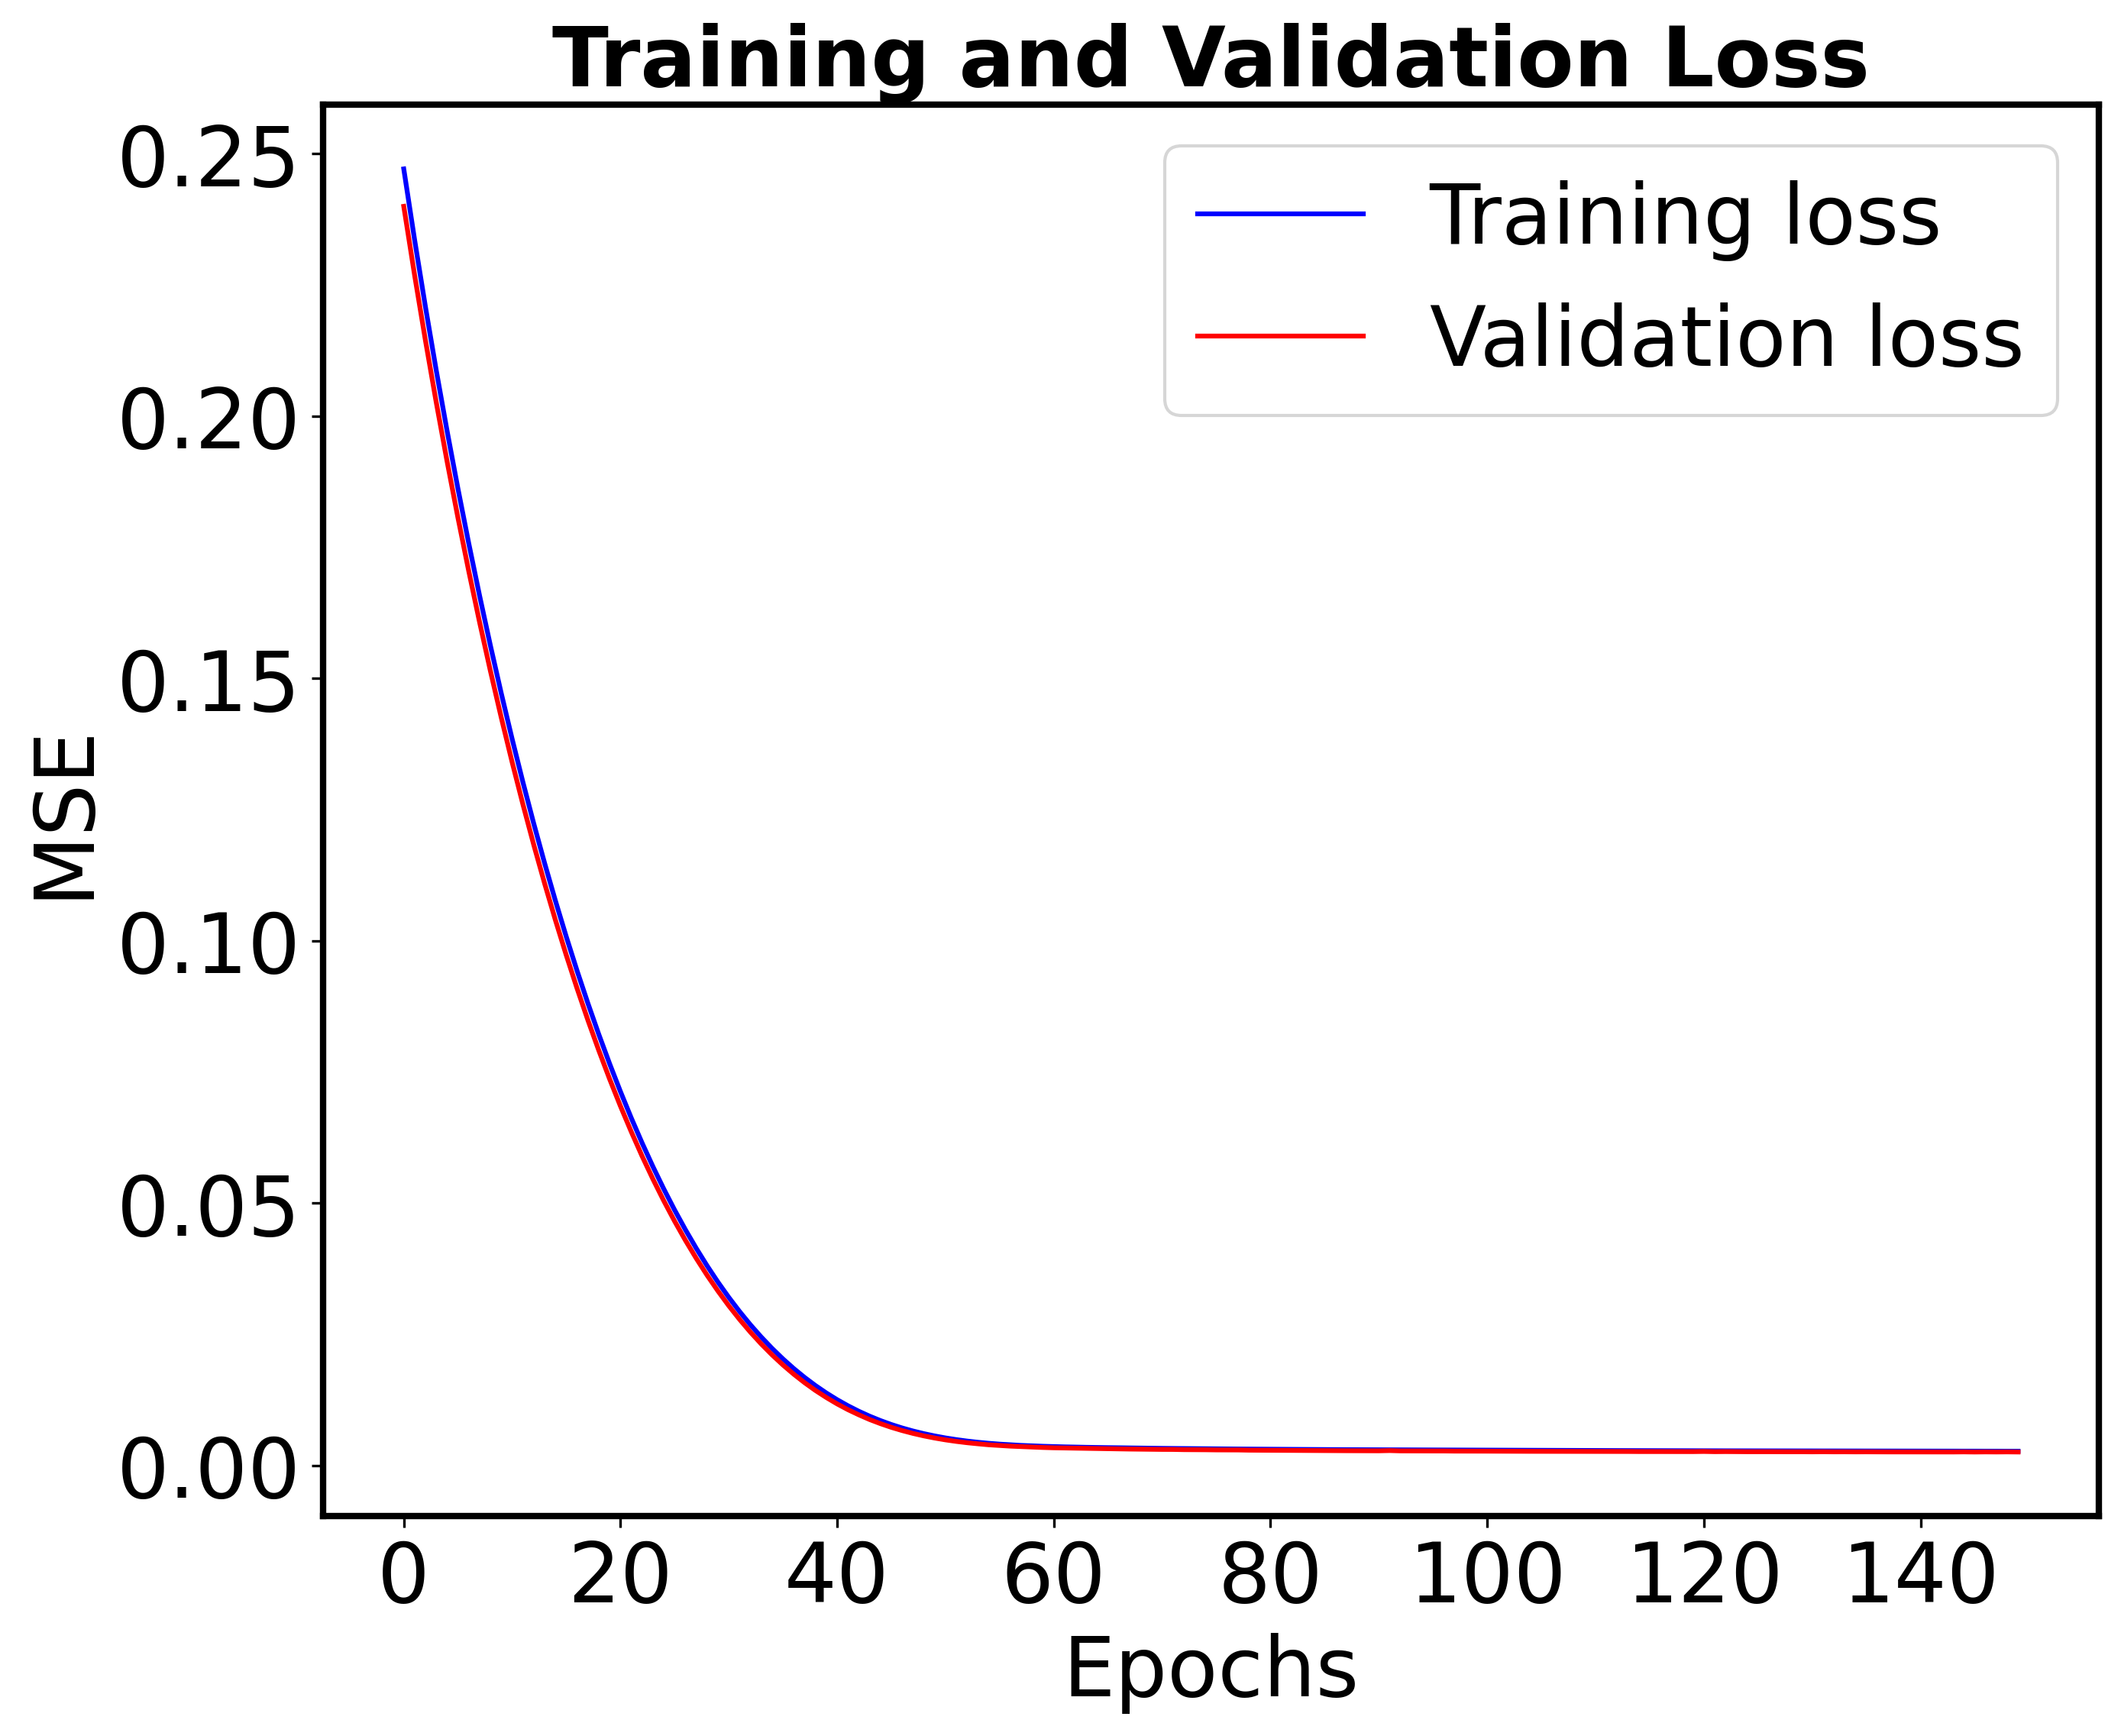
\includegraphics[width=1\linewidth]{Model2_Serie2.png}
	\caption{Model 2 - Serie 2}
	\end{subfigure}	
	\begin{subfigure}{0.49\textwidth}
	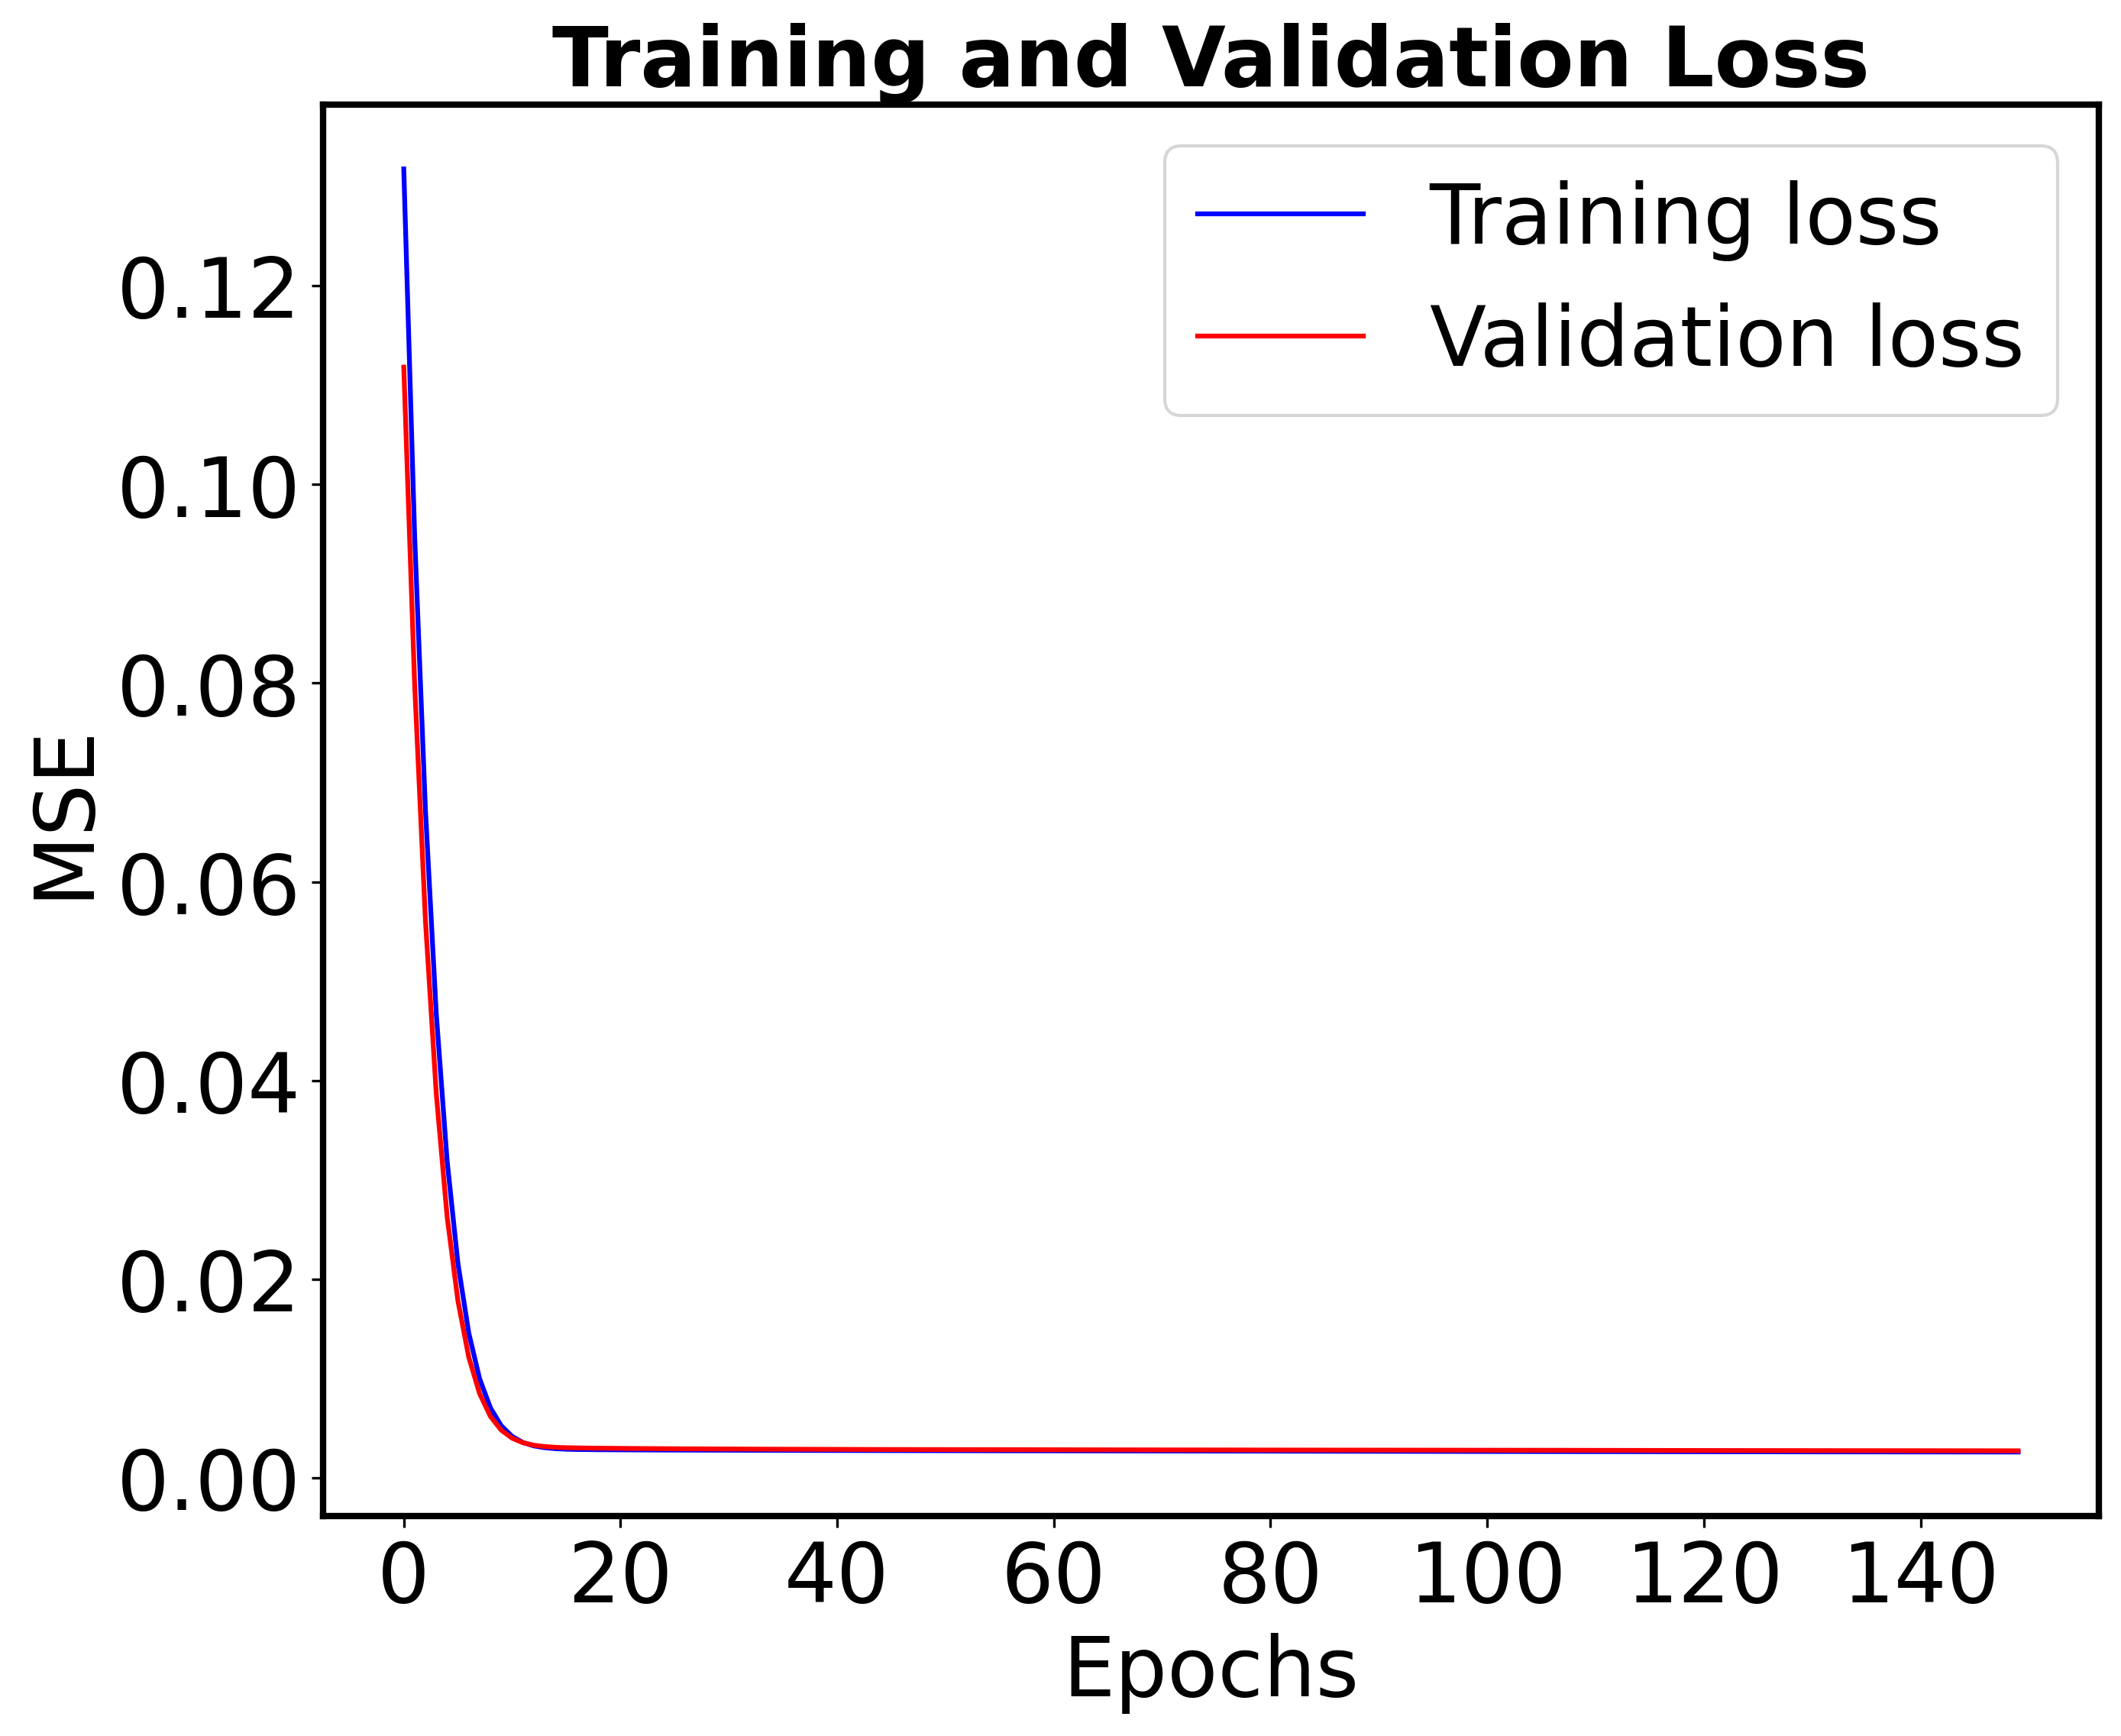
\includegraphics[width=1\linewidth]{Model3_Serie2.png}
	\caption{Model 3 - Serie 2}
	\end{subfigure}
	\caption{The evolution of the MSE on the training and validation sets.}
	\label{fig:training_validation}
\end{figure}



\section{Performance on the test set}
In this section the results on the test set are discussed for the models that were selected in section \ref{s:Model selection}. 
Also, the two best baseline models ``mean forecast'' and ``MAPE forecast'', that were explained in Section \ref{s:Baseline models}, are included in the comparison. An advantage that the baseline models have in comparison to the LSTM neural networks is that they use the previous data till the day to forecast to make predictions while the LSTM neural networks only trains on data till November. (Seeding not taken into account) This is because it needs data for the validation set to tune parameters and implement early stopping. \\

The baseline models and the LSTM neural networks both belong to a different group of models respectively to the lazy models and eager models. A lazy model only looks at the data when the query is known i.e. what day to forecast. For example a ``mean forecast'' looks after it knows which day to forecast to the same weekdays and takes the average. In comparison an eager model already makes generalizations on a training set before it knows which day it has to predict. This applies to the LSTM models.\\

Model 1 and Model 2 make use of a lag value of $ 48 $ or $ 96 $ and no seeding. When the day after a missing day(s) is predicted the inputs used during prediction could originate entirely from an estimated reference signal for the missing day(s). If this is the case, it is expected that the error on the desired day will be larger. The estimation of the reference signal is done by substituting the missing values as described in Section \ref{s:Preprocessing_cha4}. For both Serie 1 and Serie 2 there are $ 8 $ missing days in the test set.

\begin{figure}[h]
	\centering
	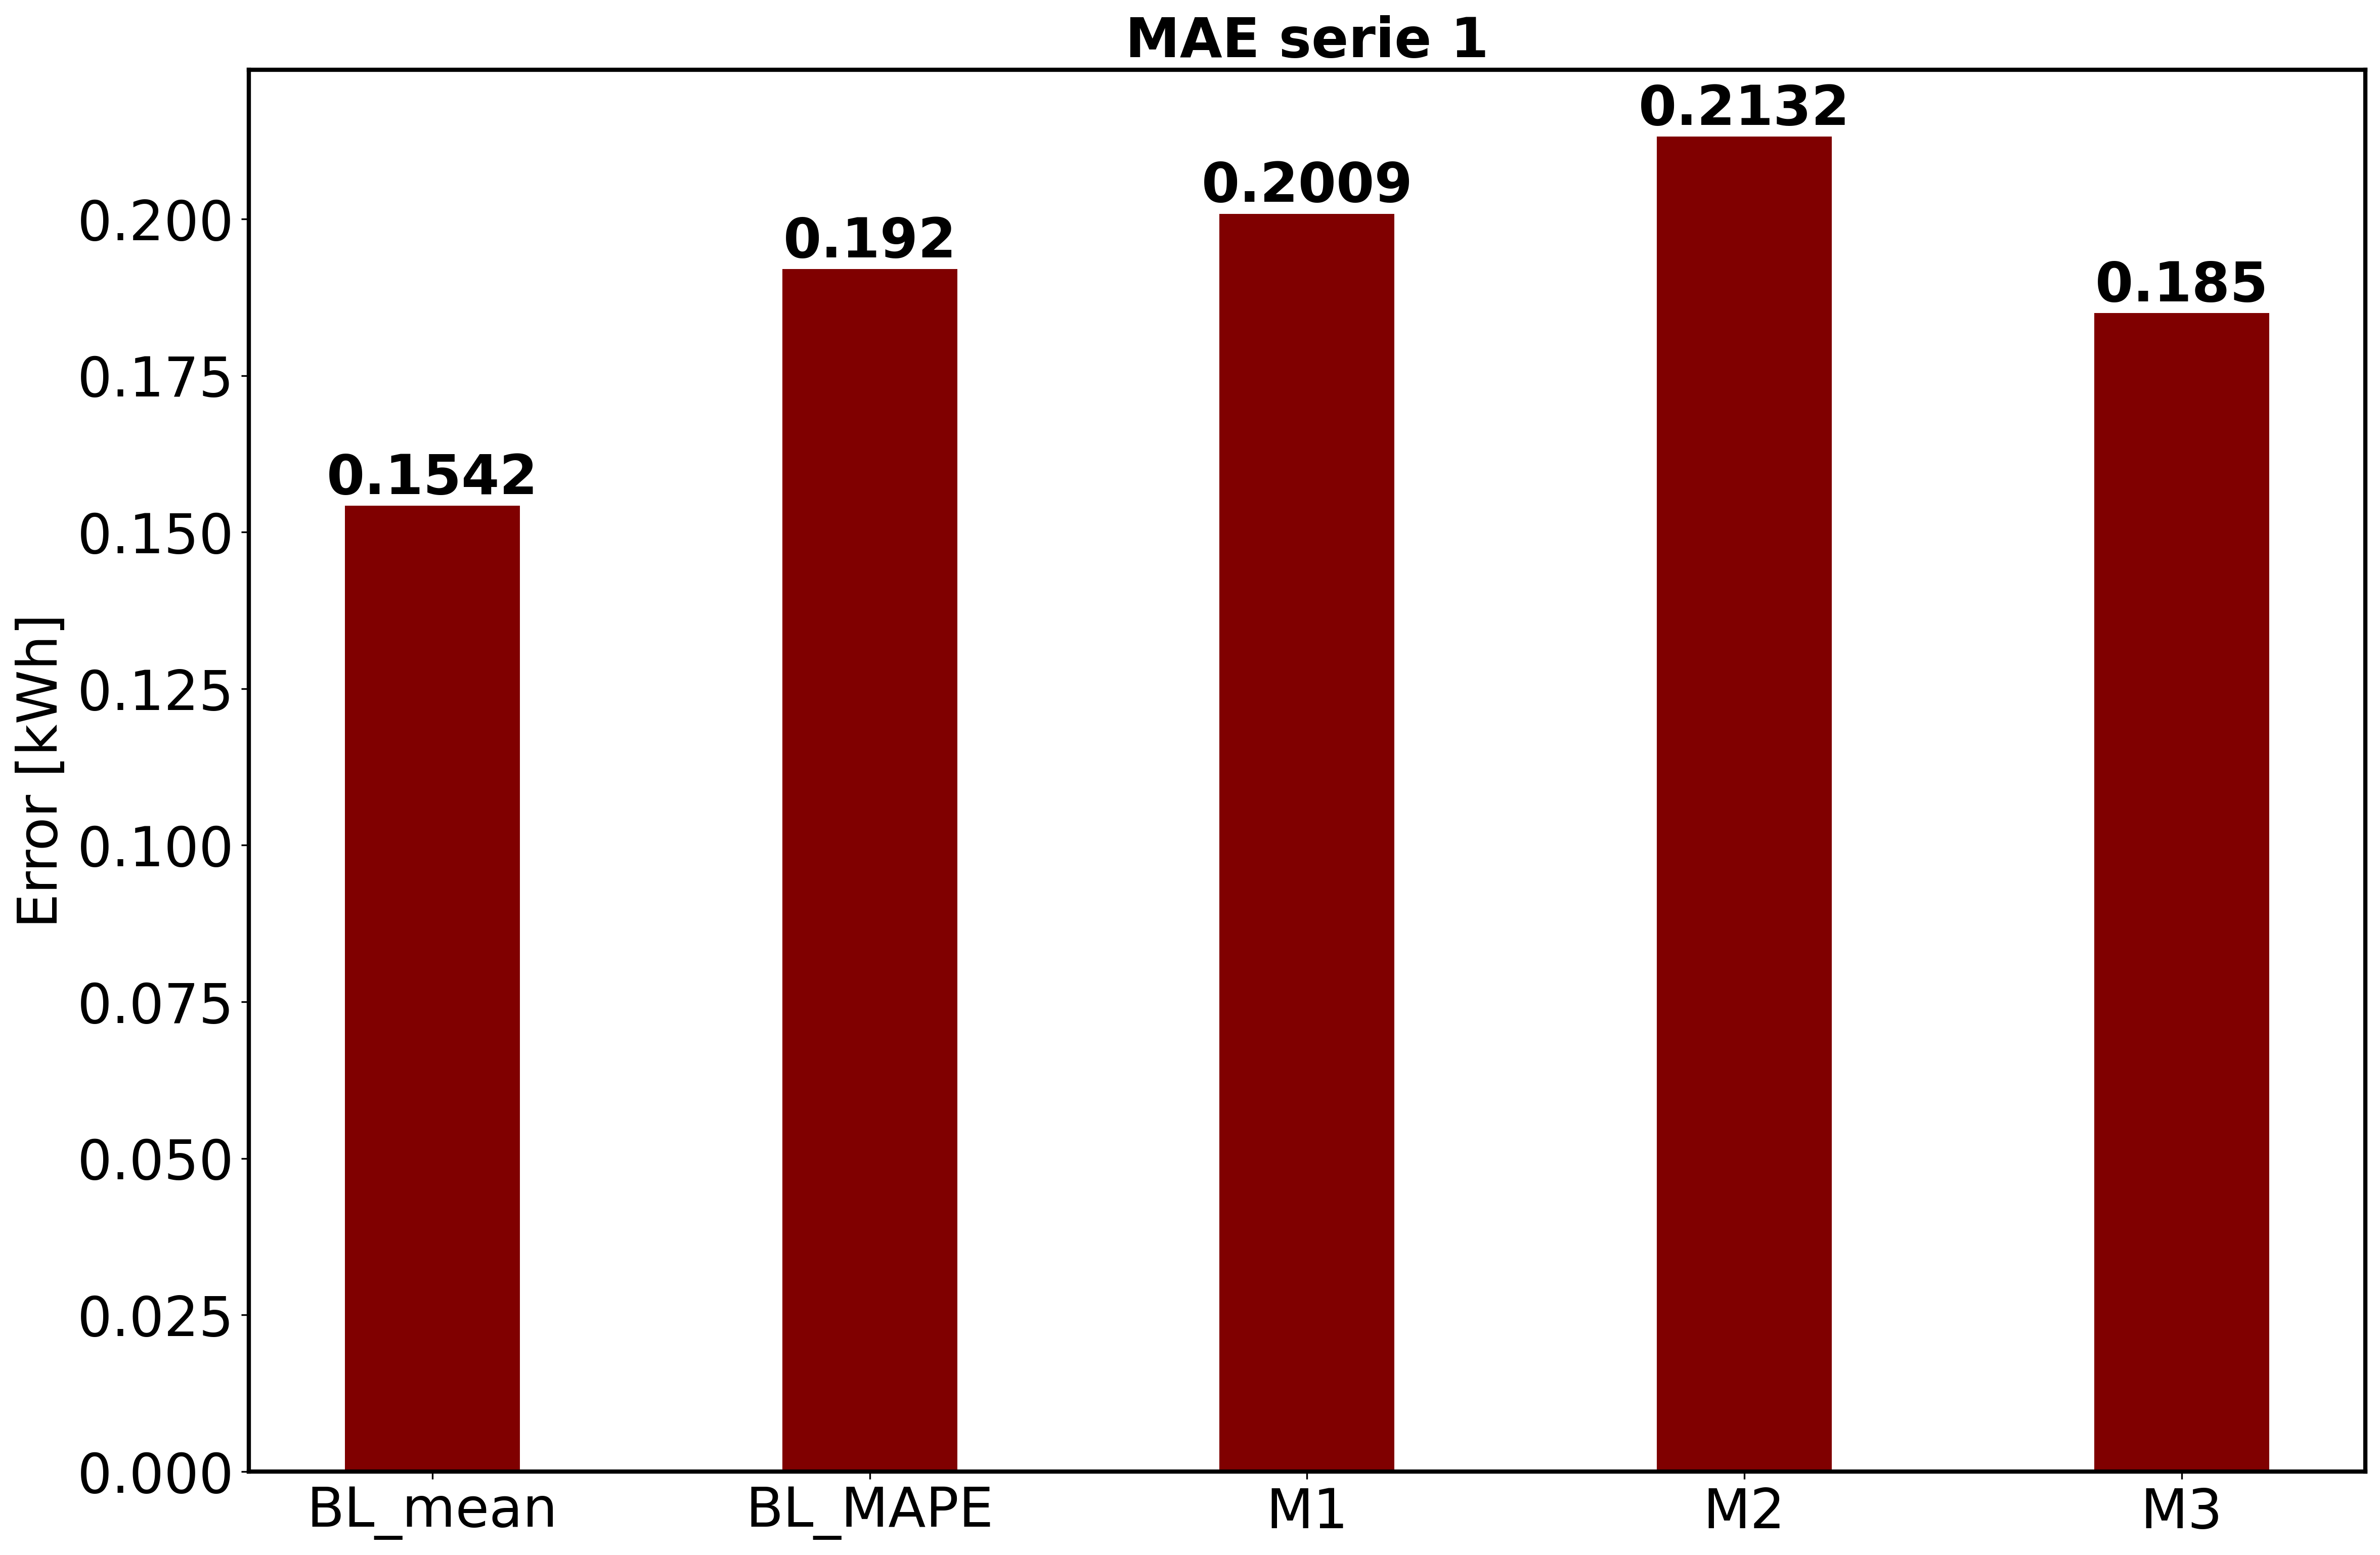
\includegraphics[width=0.8\linewidth]{MAE_1.png}
	\caption{The MAE performance on all the days of the test set for Serie 1.}
	\label{fig:MAE_serie1}
\end{figure}

\begin{figure}[h]
	\centering
	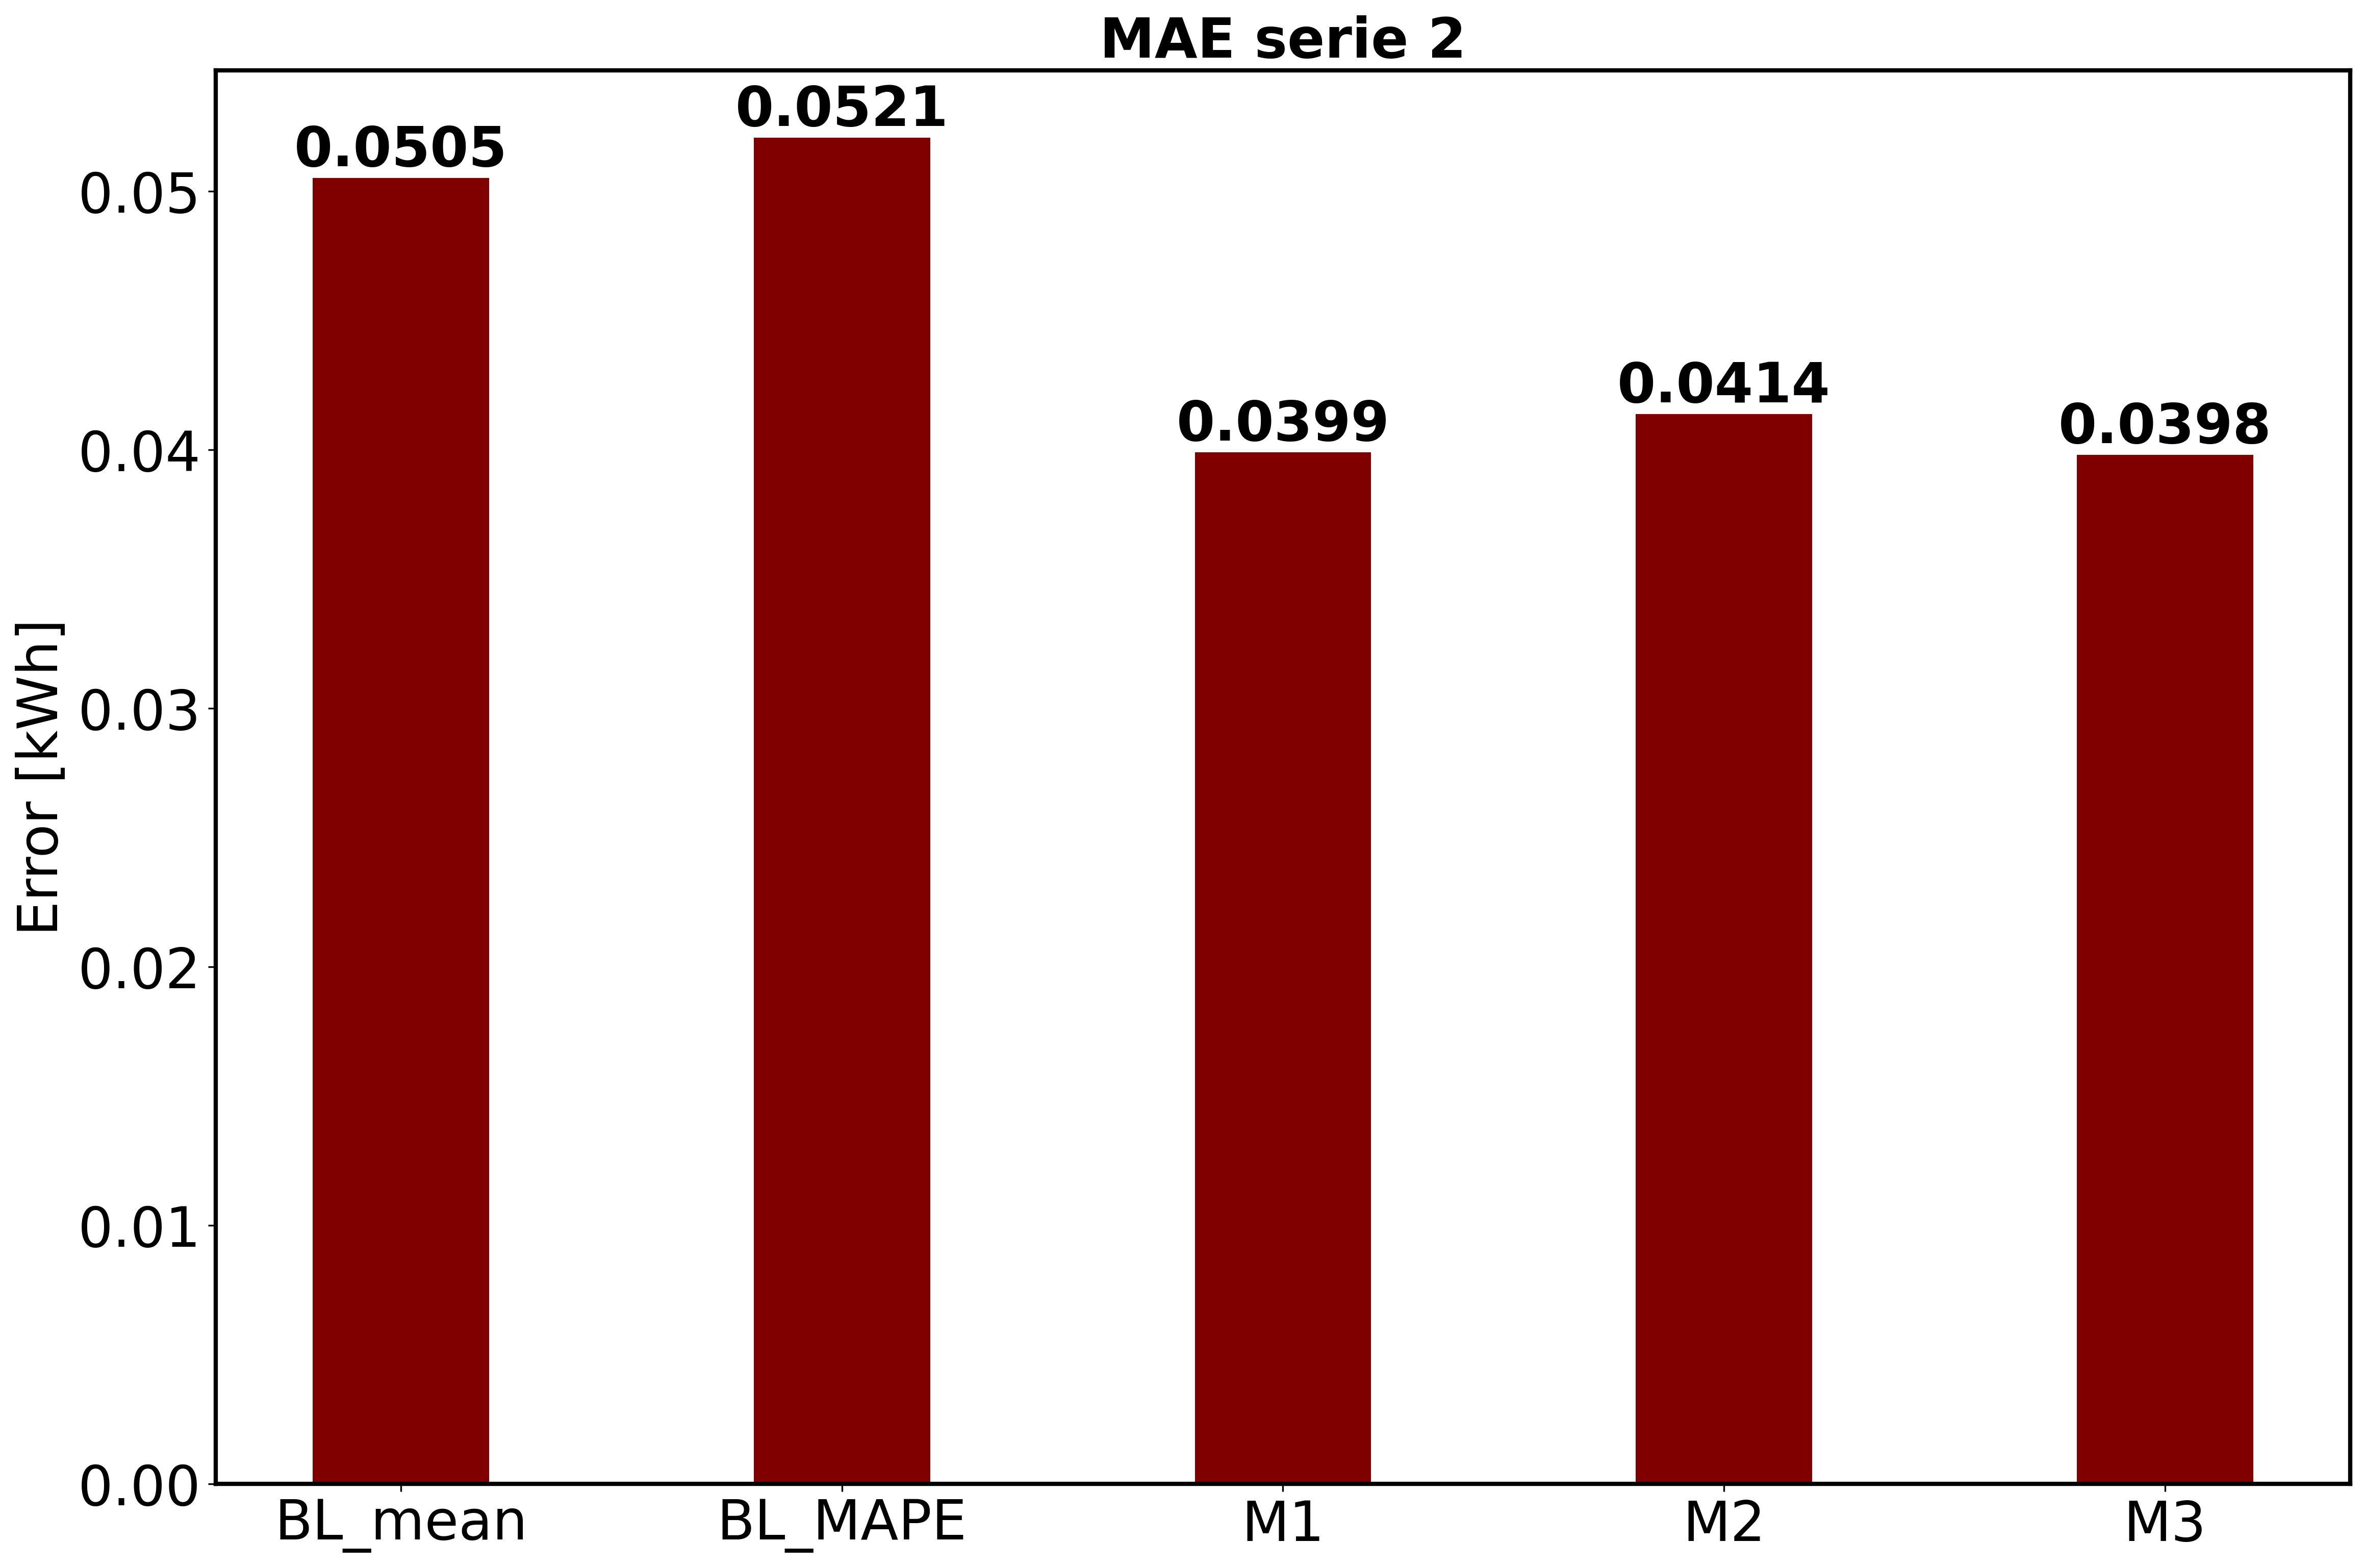
\includegraphics[width=0.8\linewidth]{MAE_2.png}
	\caption{The MAE performance on all the days of the test set for Serie 2.}
	\label{fig:MAE_serie2}
\end{figure}	

\begin{figure}[h]
	\centering
	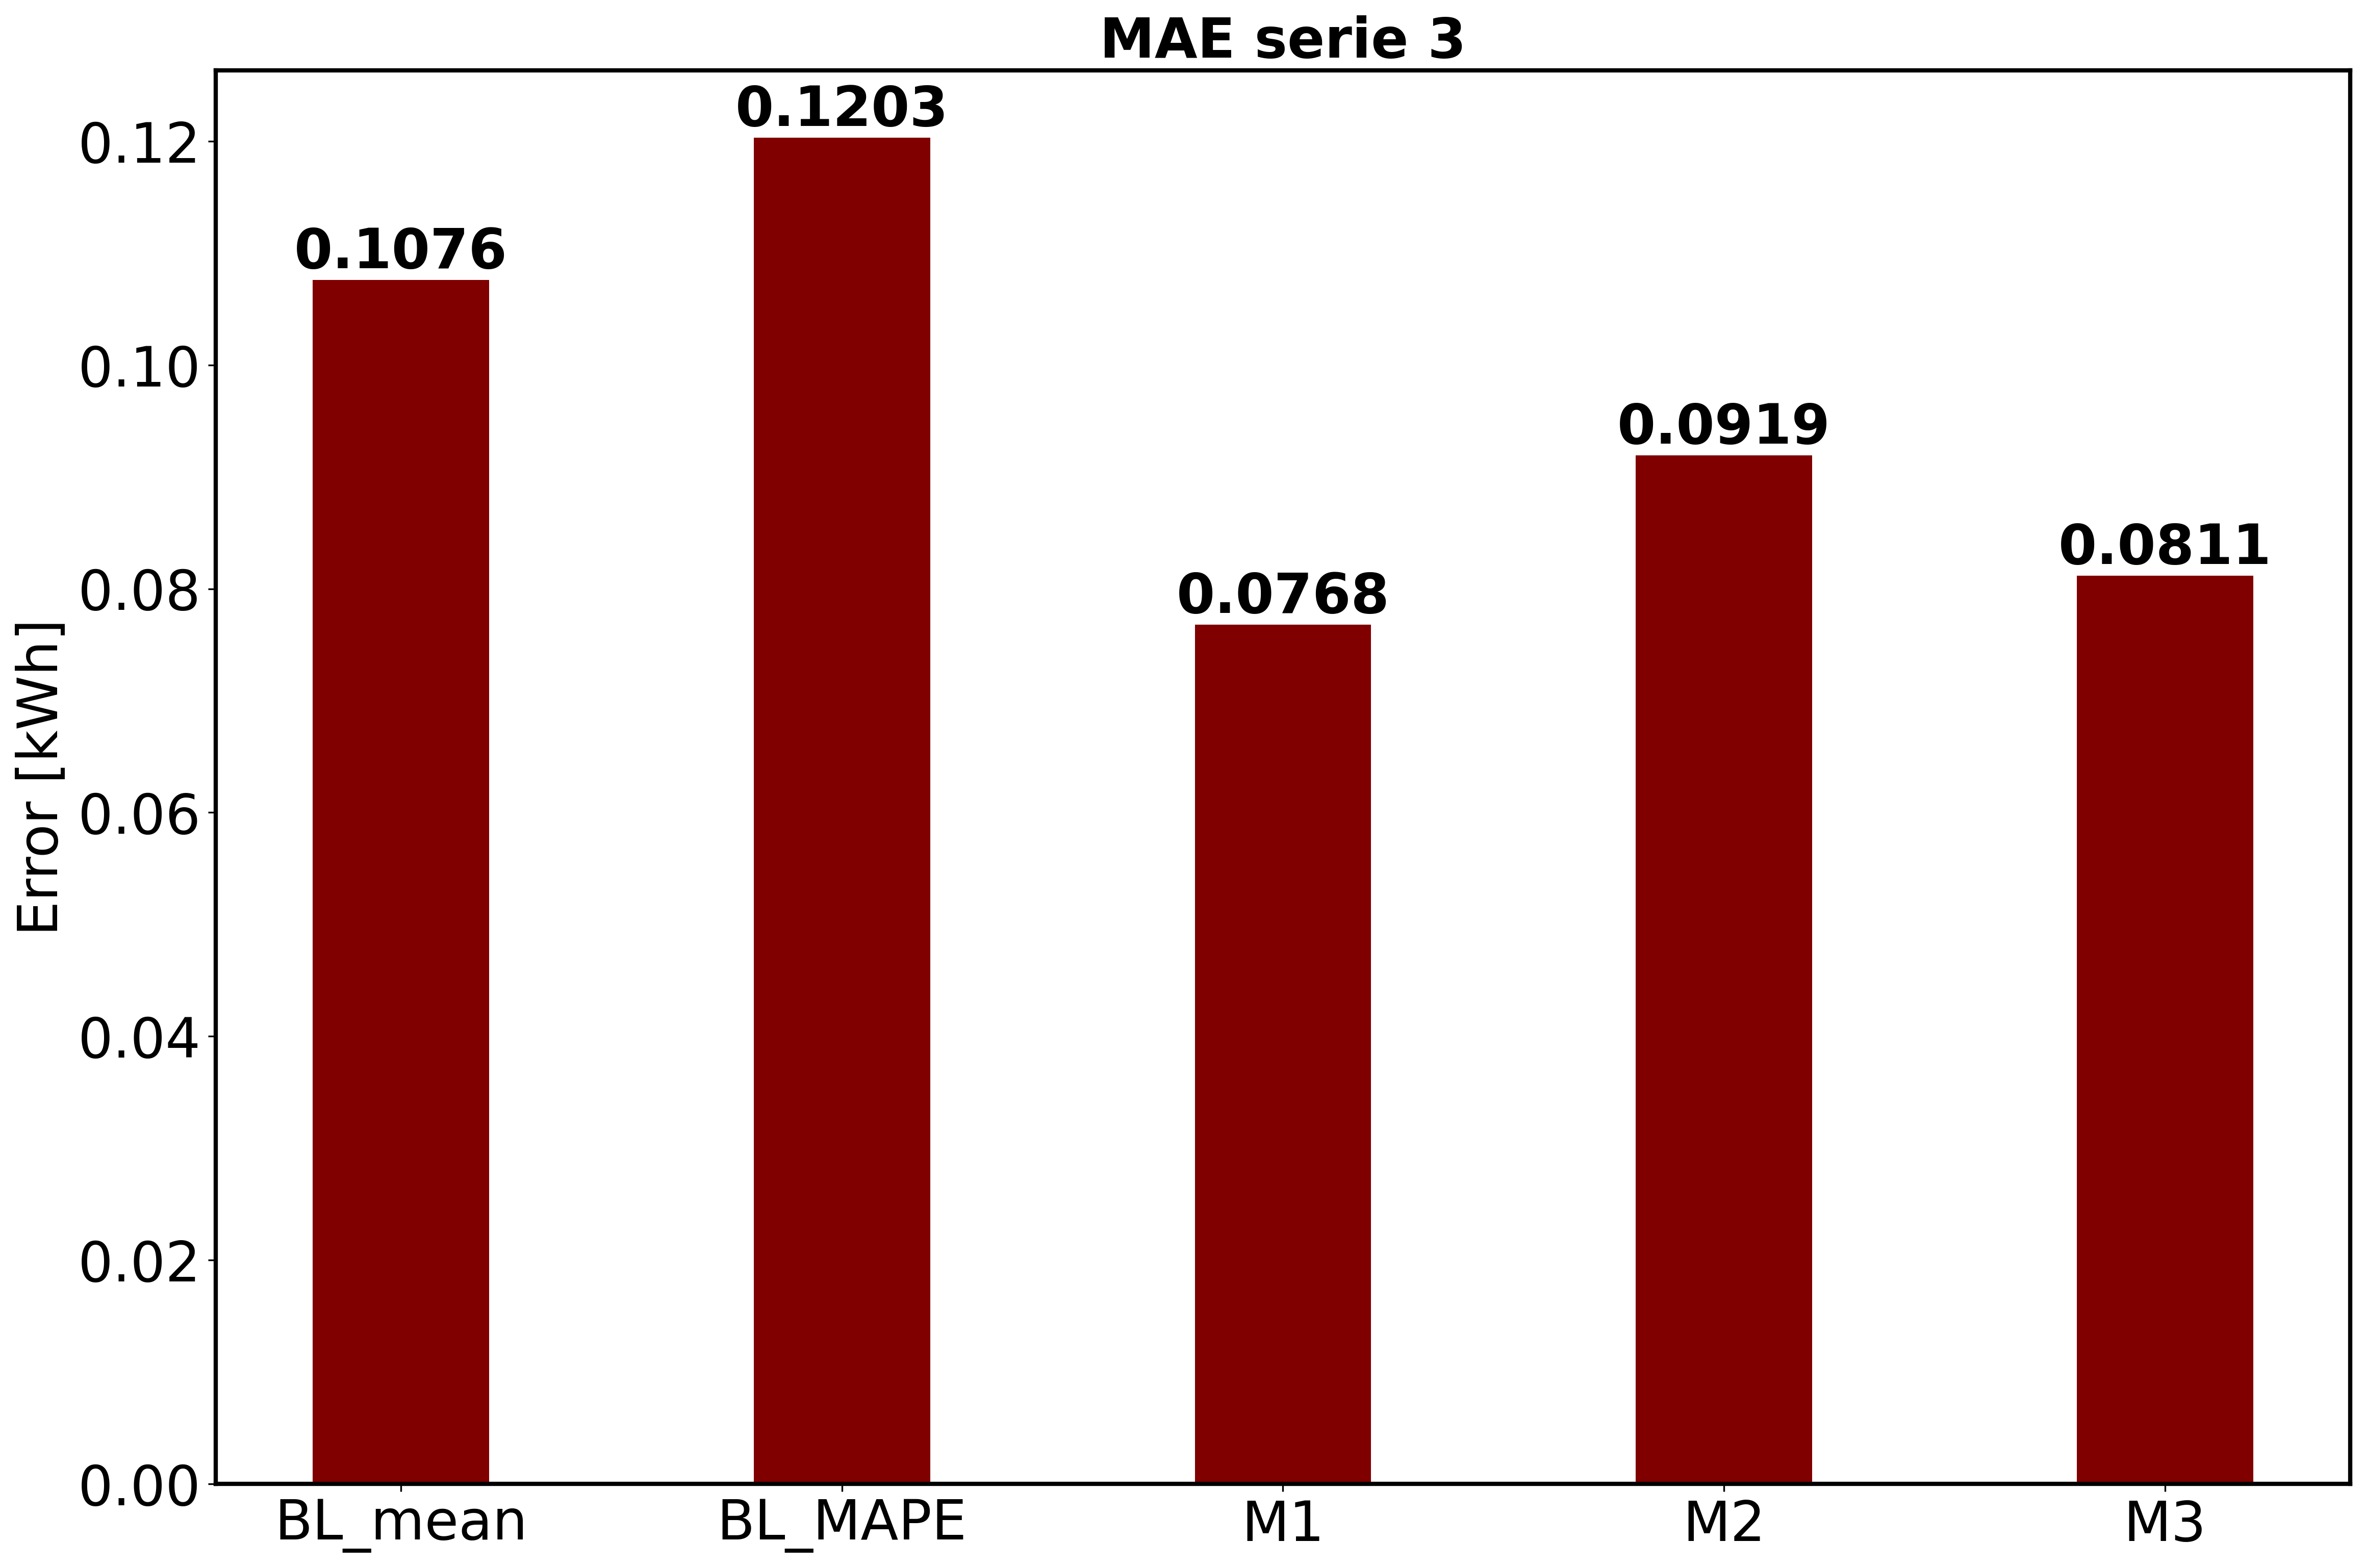
\includegraphics[width=0.8\linewidth]{MAE_3.png}
	\caption{The MAE performance on all the days of the test set for Serie 3.}
	\label{fig:MAE_serie3}
\end{figure}	

Figures \ref{fig:MAE_serie1}, \ref{fig:MAE_serie2} and \ref{fig:MAE_serie3} give a comparison of the three LSTM models and the two baseline models. It can be seen that there is a reduction of the MAE for Series 2 and 3 for all the LSTM models and for Serie 1, Model 3 attains a smaller error than the ``MAPE forecast'' model. Also, it can be noticed that Model 2 for all the three series behaves slightly worse than the other two LSTM models. It is clear that the performance of the models is serie dependent.\\

To get more insight in how the MAE error is distributed over the test set, it is calculated for each individual day and displayed in Figures \ref{fig:MAE_line_serie1}, \ref{fig:MAE_line_serie2} and \ref{fig:MAE_line_serie3} in Appendix \ref{app:Extensions on the evaluation results}. Figures \ref{fig:MAE_line_serie2} and \ref{fig:MAE_line_serie3} are discontinuous due to the missing days that are present in the reference signal in the month December. When the reference values of a day are not known, the day is removed from the test set to remove an additional estimation error of the reference signal during the calculation of the MAE. This is also the case for the calculation of the MAE in Figures \ref{fig:MAE_serie1}, \ref{fig:MAE_serie2} and \ref{fig:MAE_serie3}. \\

Next, it is noted that the MAPE for the LSTM models is much higher than for the baseline models as is shown in Table \ref{tab:summary_MAPE_error}. As displayed in Figure \ref{fig:individual_forecasts} this is due to an overestimation of the reference signal when the values are small.\\


\begin{table}[h]
	\centering
	\begin{tabular}{@{}l|ccccc@{}} \toprule
		&\textbf{Mean forecast} & \textbf{MAPE forecast} & \textbf{Model $ 1 $} & \textbf{Model $ 2 $} & \textbf{Model $ 3 $}\\\midrule
		\textbf{Serie 1} & $0.46 $&$ 0.41$  & $3.07 $ & $3.37 $  & $3.27 $\\
		\textbf{Serie 2} & $1.82 $&$ 0.83 $  & $3.67$ & $3.64 $  & $3.65 $\\
		\textbf{Serie 3} & $0.80 $&$ 0.48 $  & $3.30$ & $3.44 $ & $3.21 $\\\bottomrule
	\end{tabular}
	\caption{The MAPE for each Model and serie.}
	\label{tab:summary_MAPE_error}
\end{table}

To get better insight in the actual output of the different models, Figure \ref{fig:individual_forecasts} shows the prediction of the different models on a chosen day in the test set.\\
 
 \begin{figure}[ht]
 	\begin{subfigure}{0.32\textwidth}
 		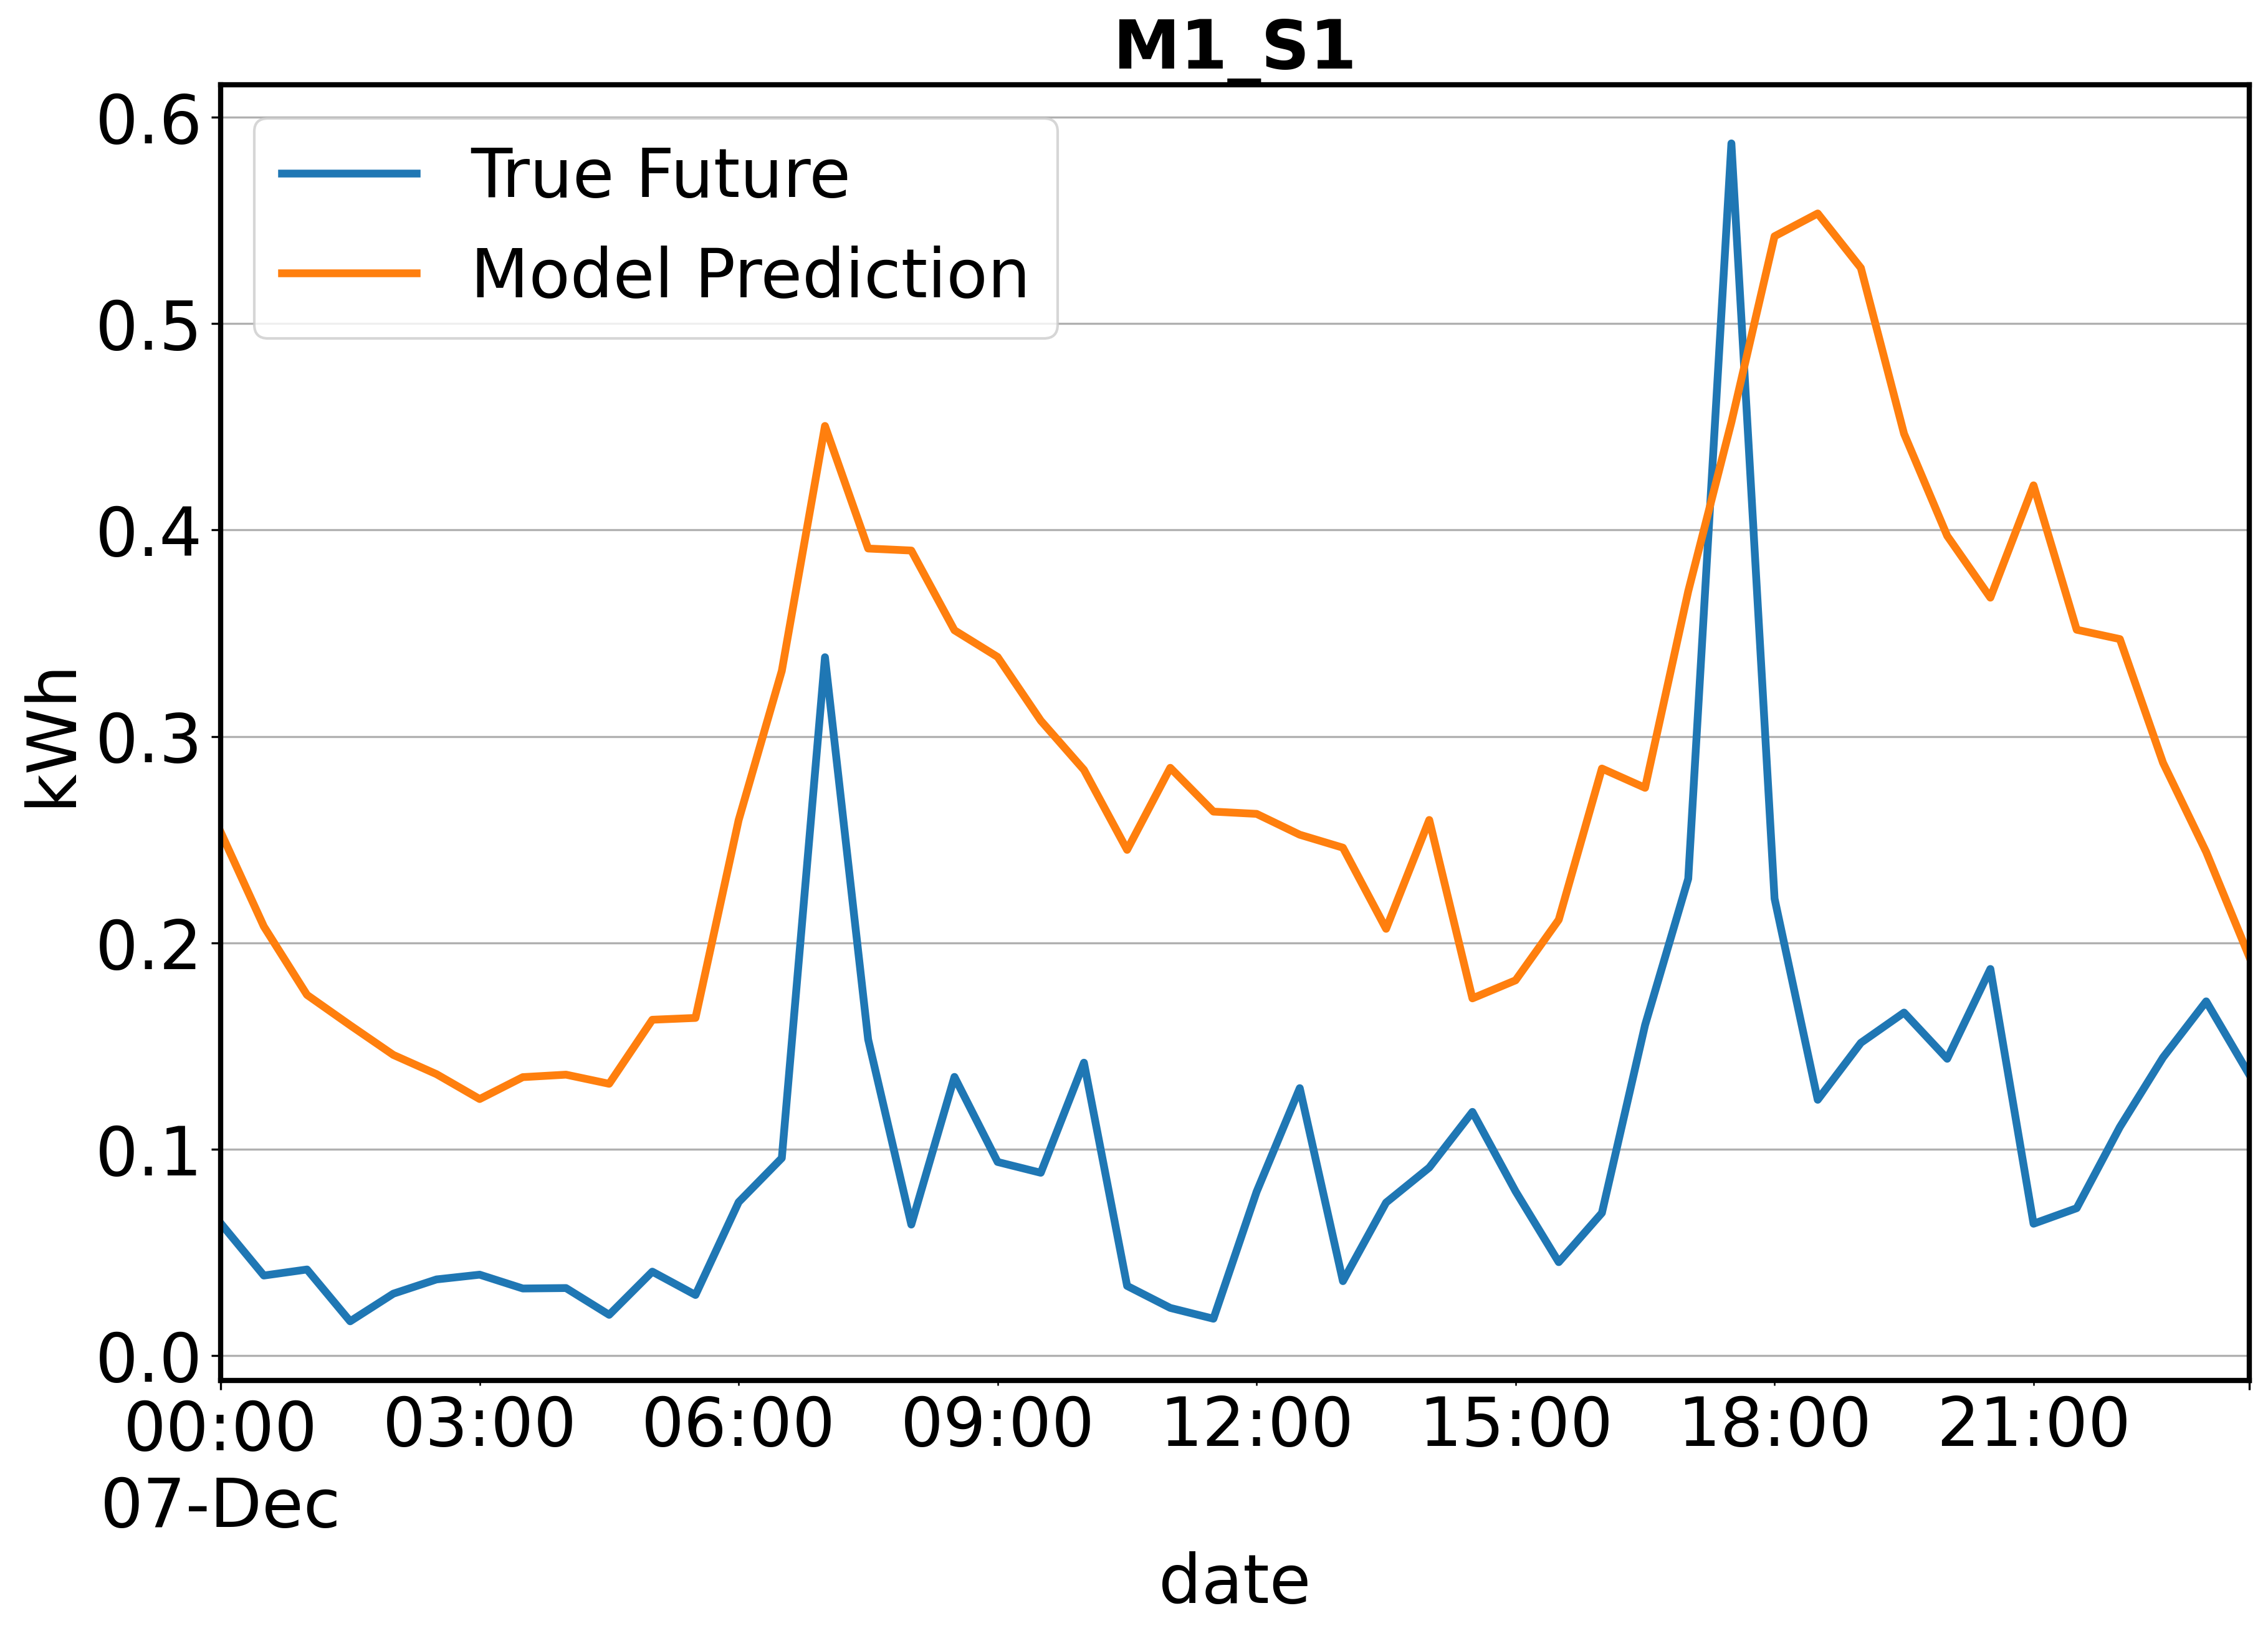
\includegraphics[width=1\linewidth]{IDM1_S1_Day341.png}
 		\caption{Model $ 1 $ - Serie $ 1 $}
 	\end{subfigure}	 	
 	\begin{subfigure}{0.32\textwidth}
 		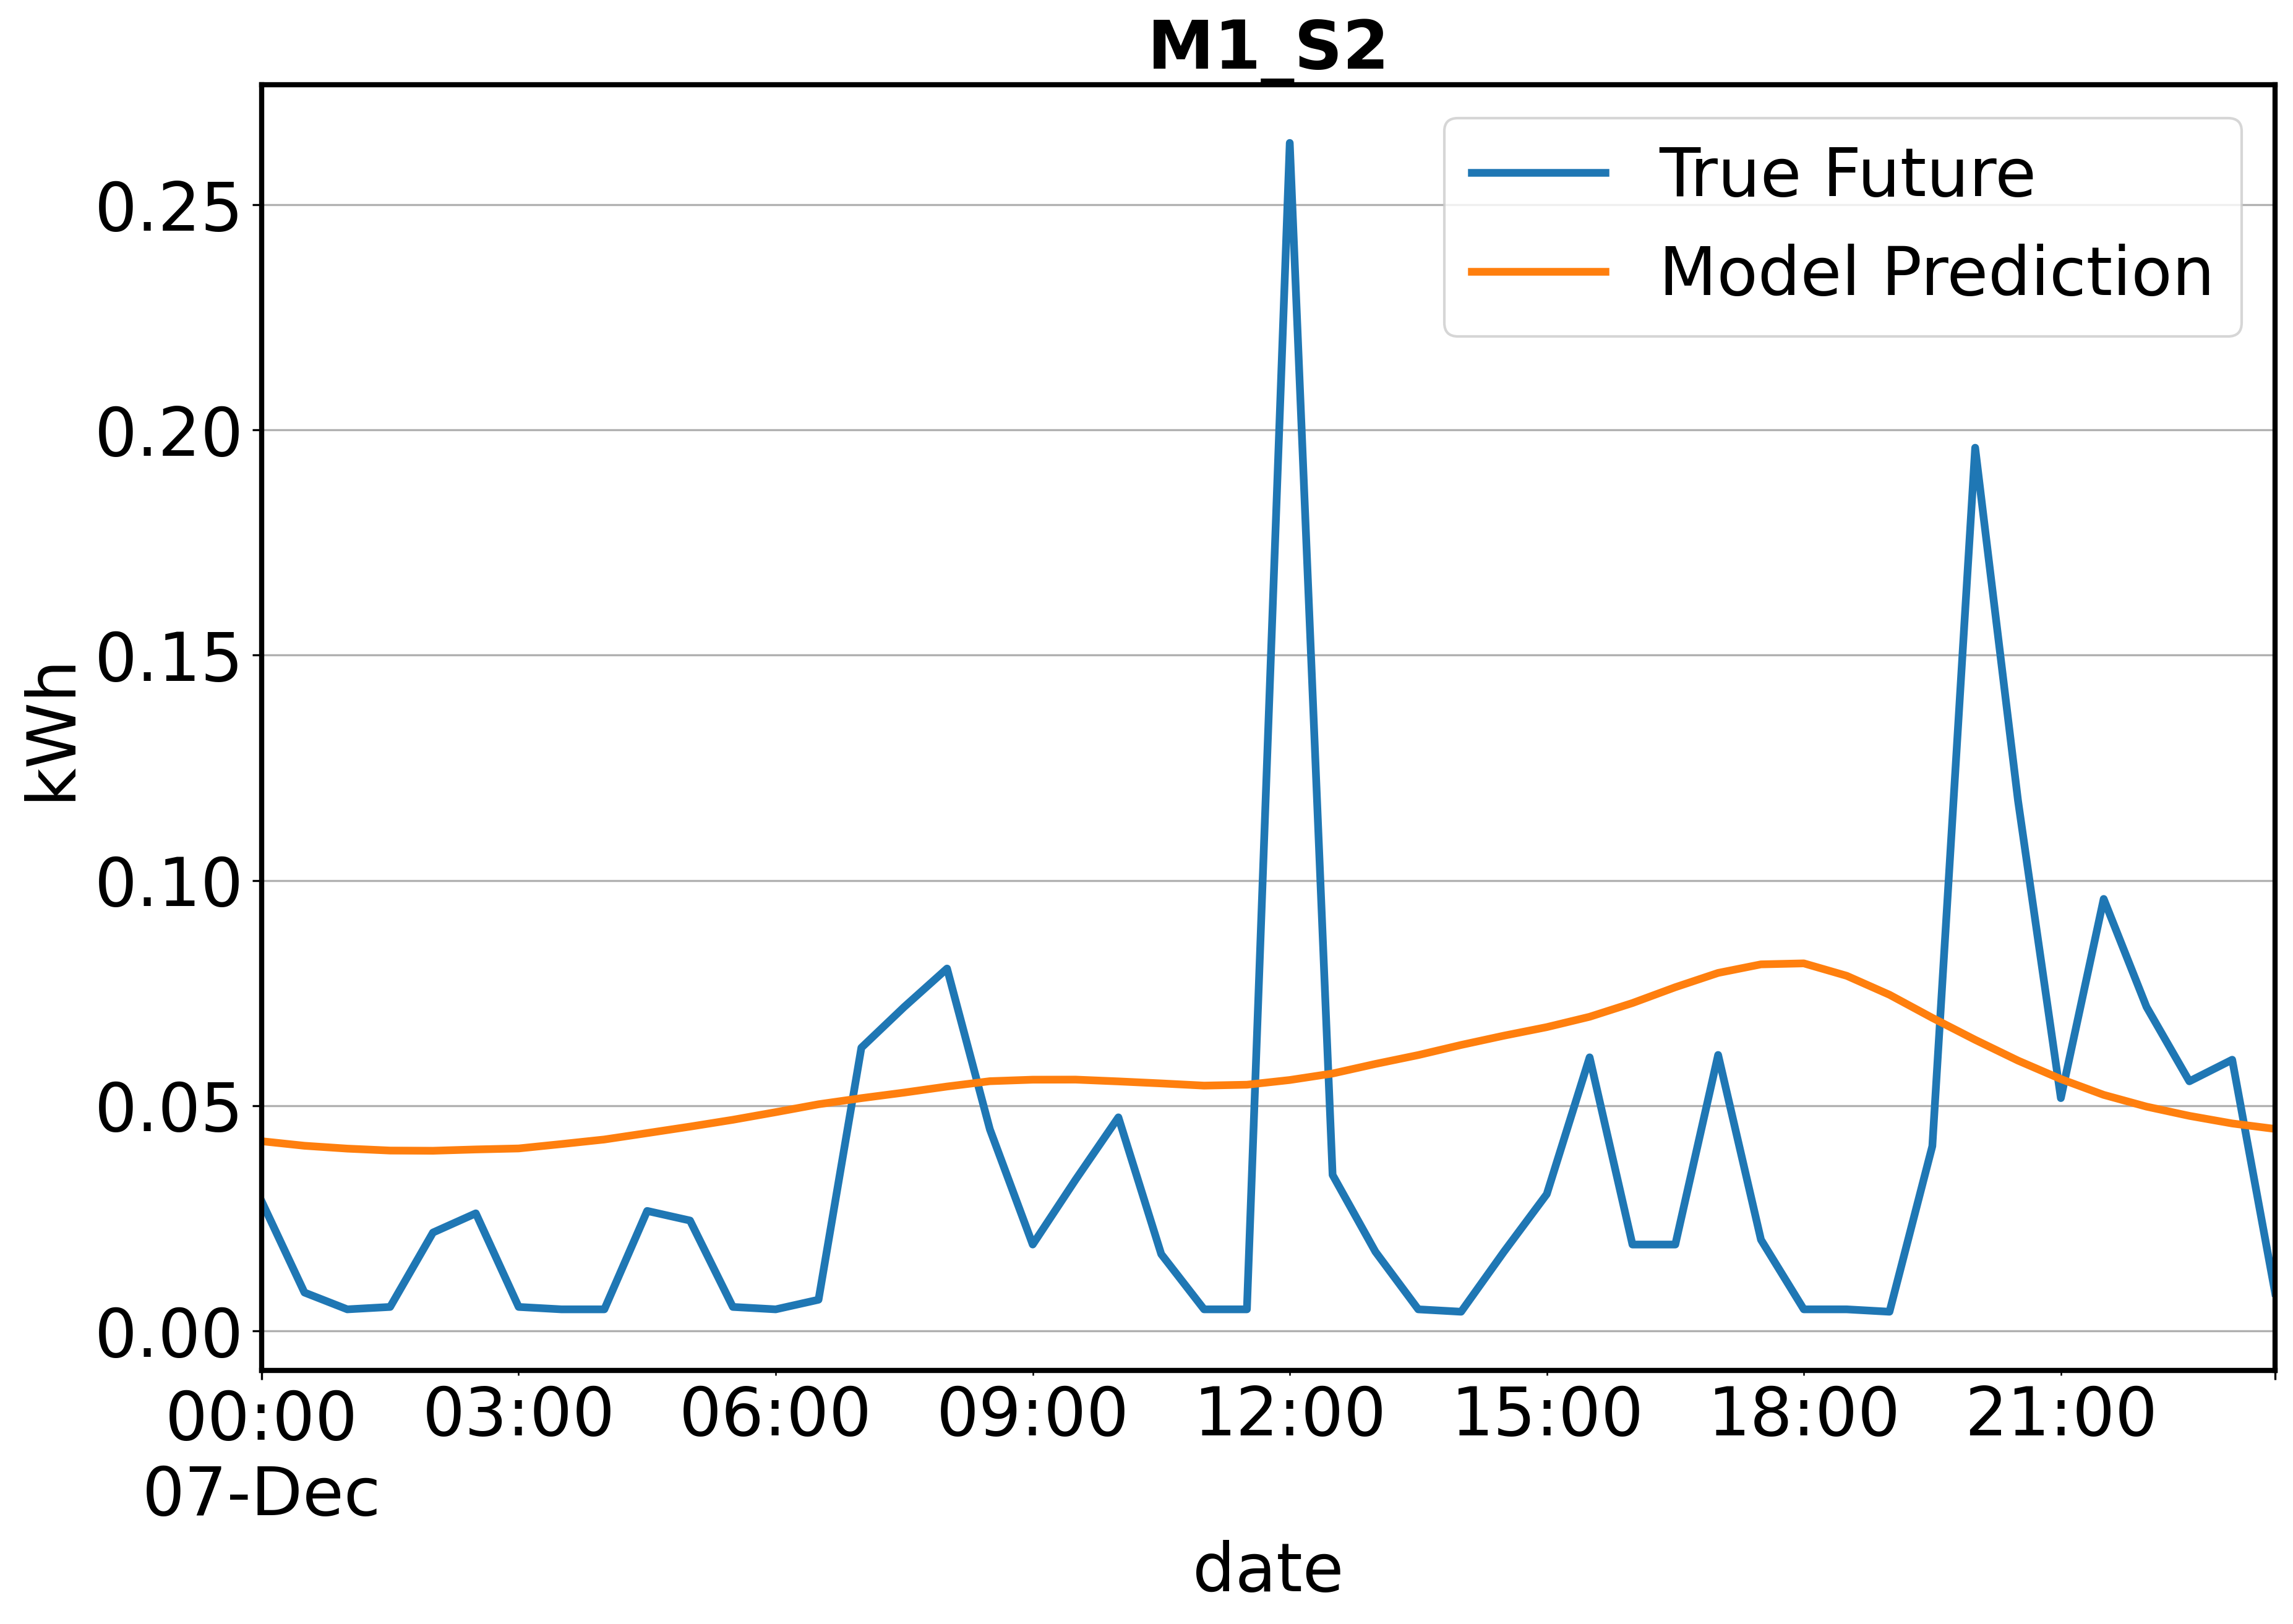
\includegraphics[width=1\linewidth]{IDM1_S2_Day341.png}
 		\caption{Model $ 1 $ - Serie $ 2 $}
 	\end{subfigure}	
 	\begin{subfigure}{0.32\textwidth}
 		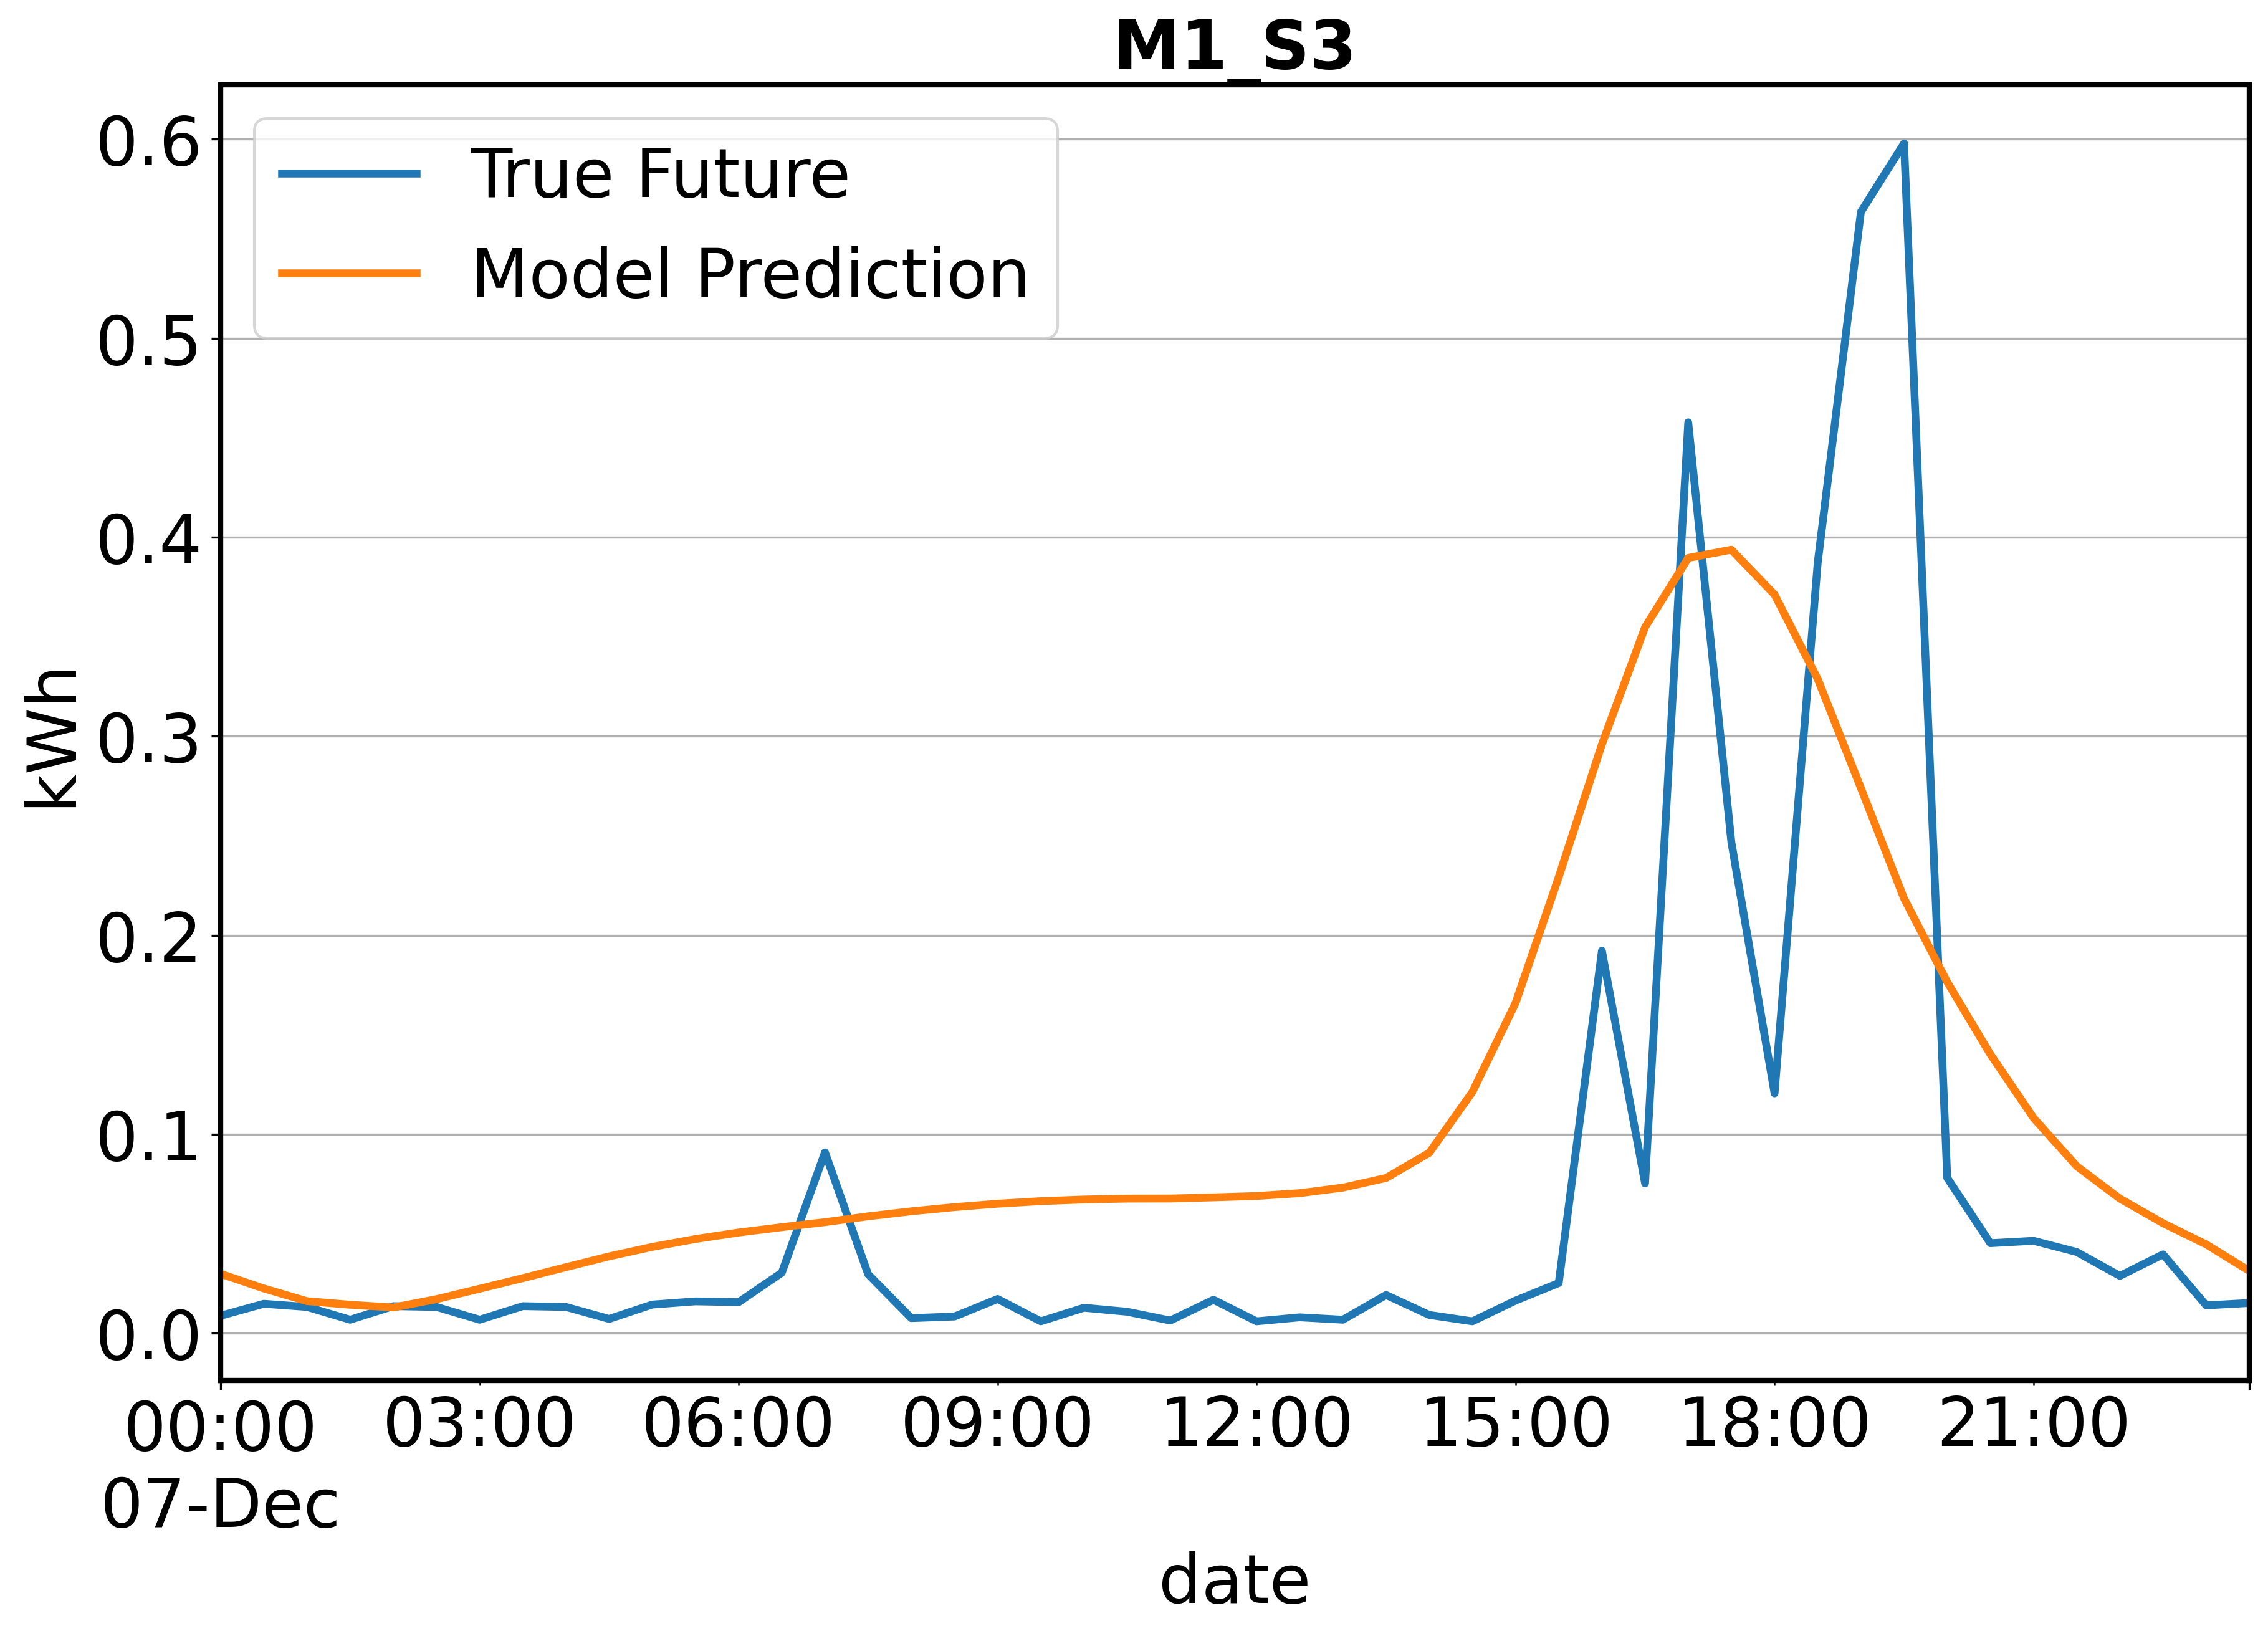
\includegraphics[width=1\linewidth]{IDM1_S3_Day341.png}
 		\caption{Model $ 1 $ - Serie $ 3 $}
 	\end{subfigure}
  	\begin{subfigure}{0.32\textwidth}
 		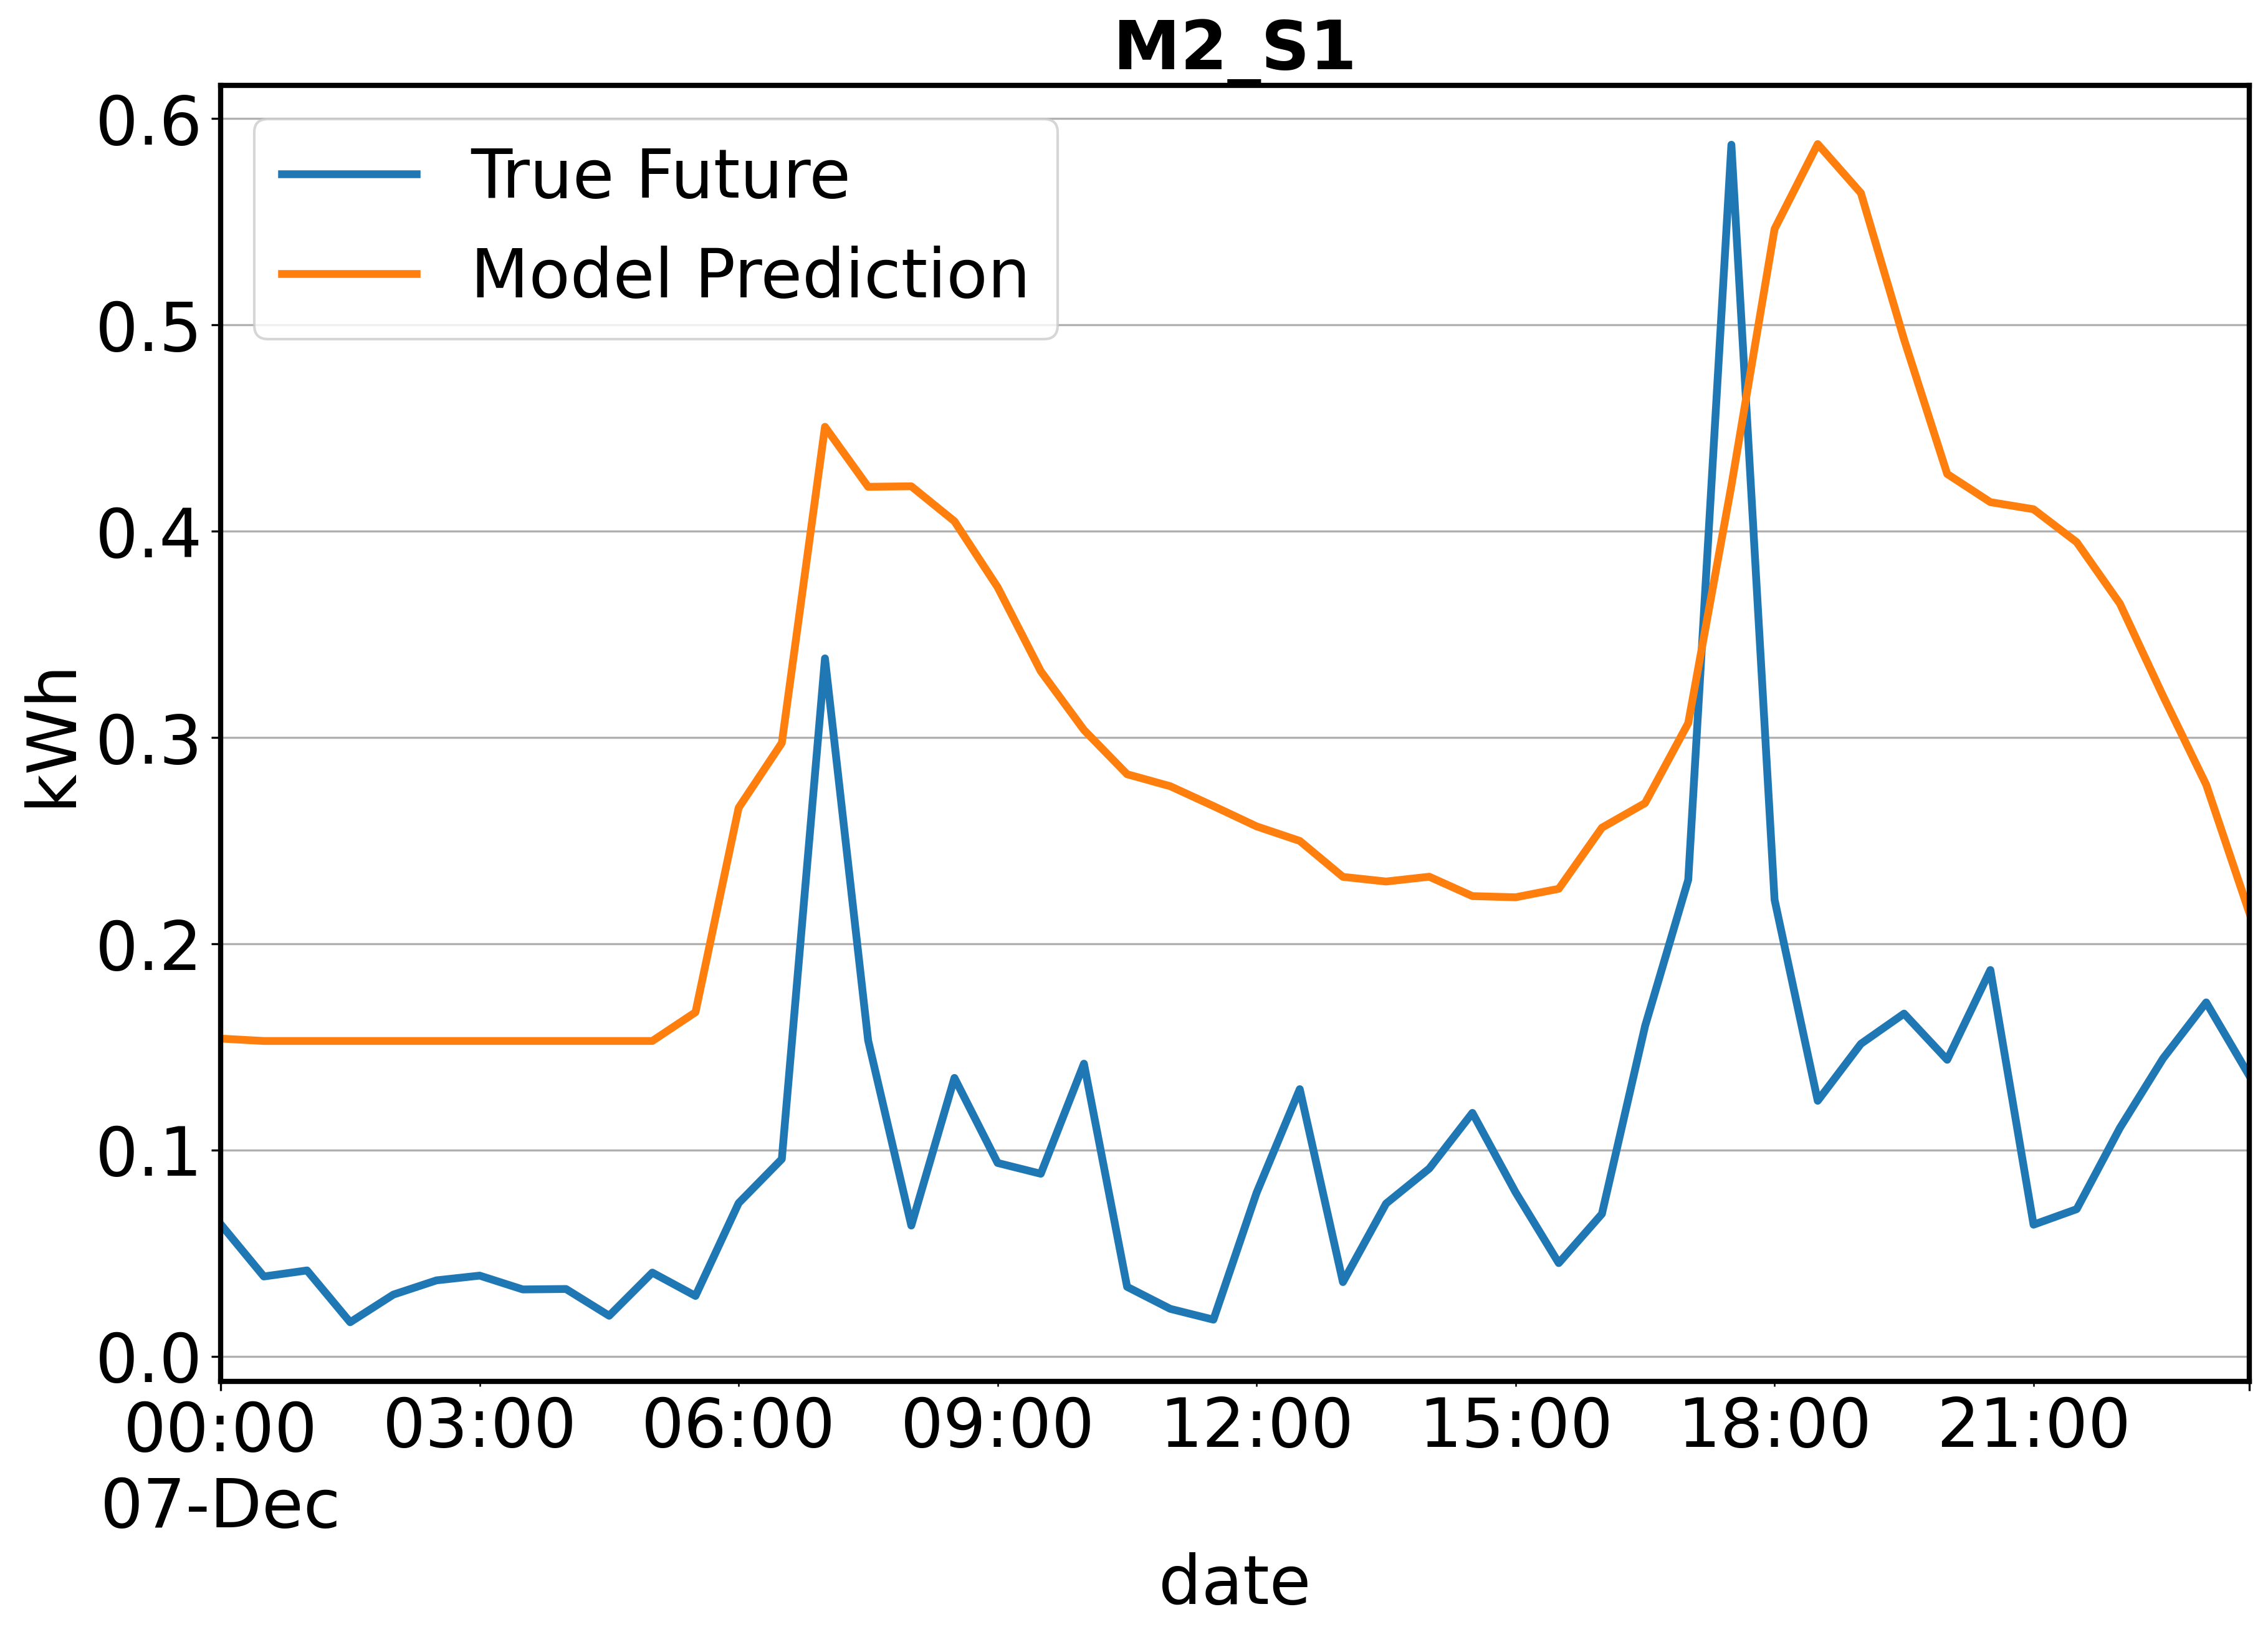
\includegraphics[width=1\linewidth]{IDM2_S1_Day341.png}
 		\caption{Model $ 2 $ - Serie $ 1 $}
 	\end{subfigure}	 	
	 \begin{subfigure}{0.32\textwidth}
	 	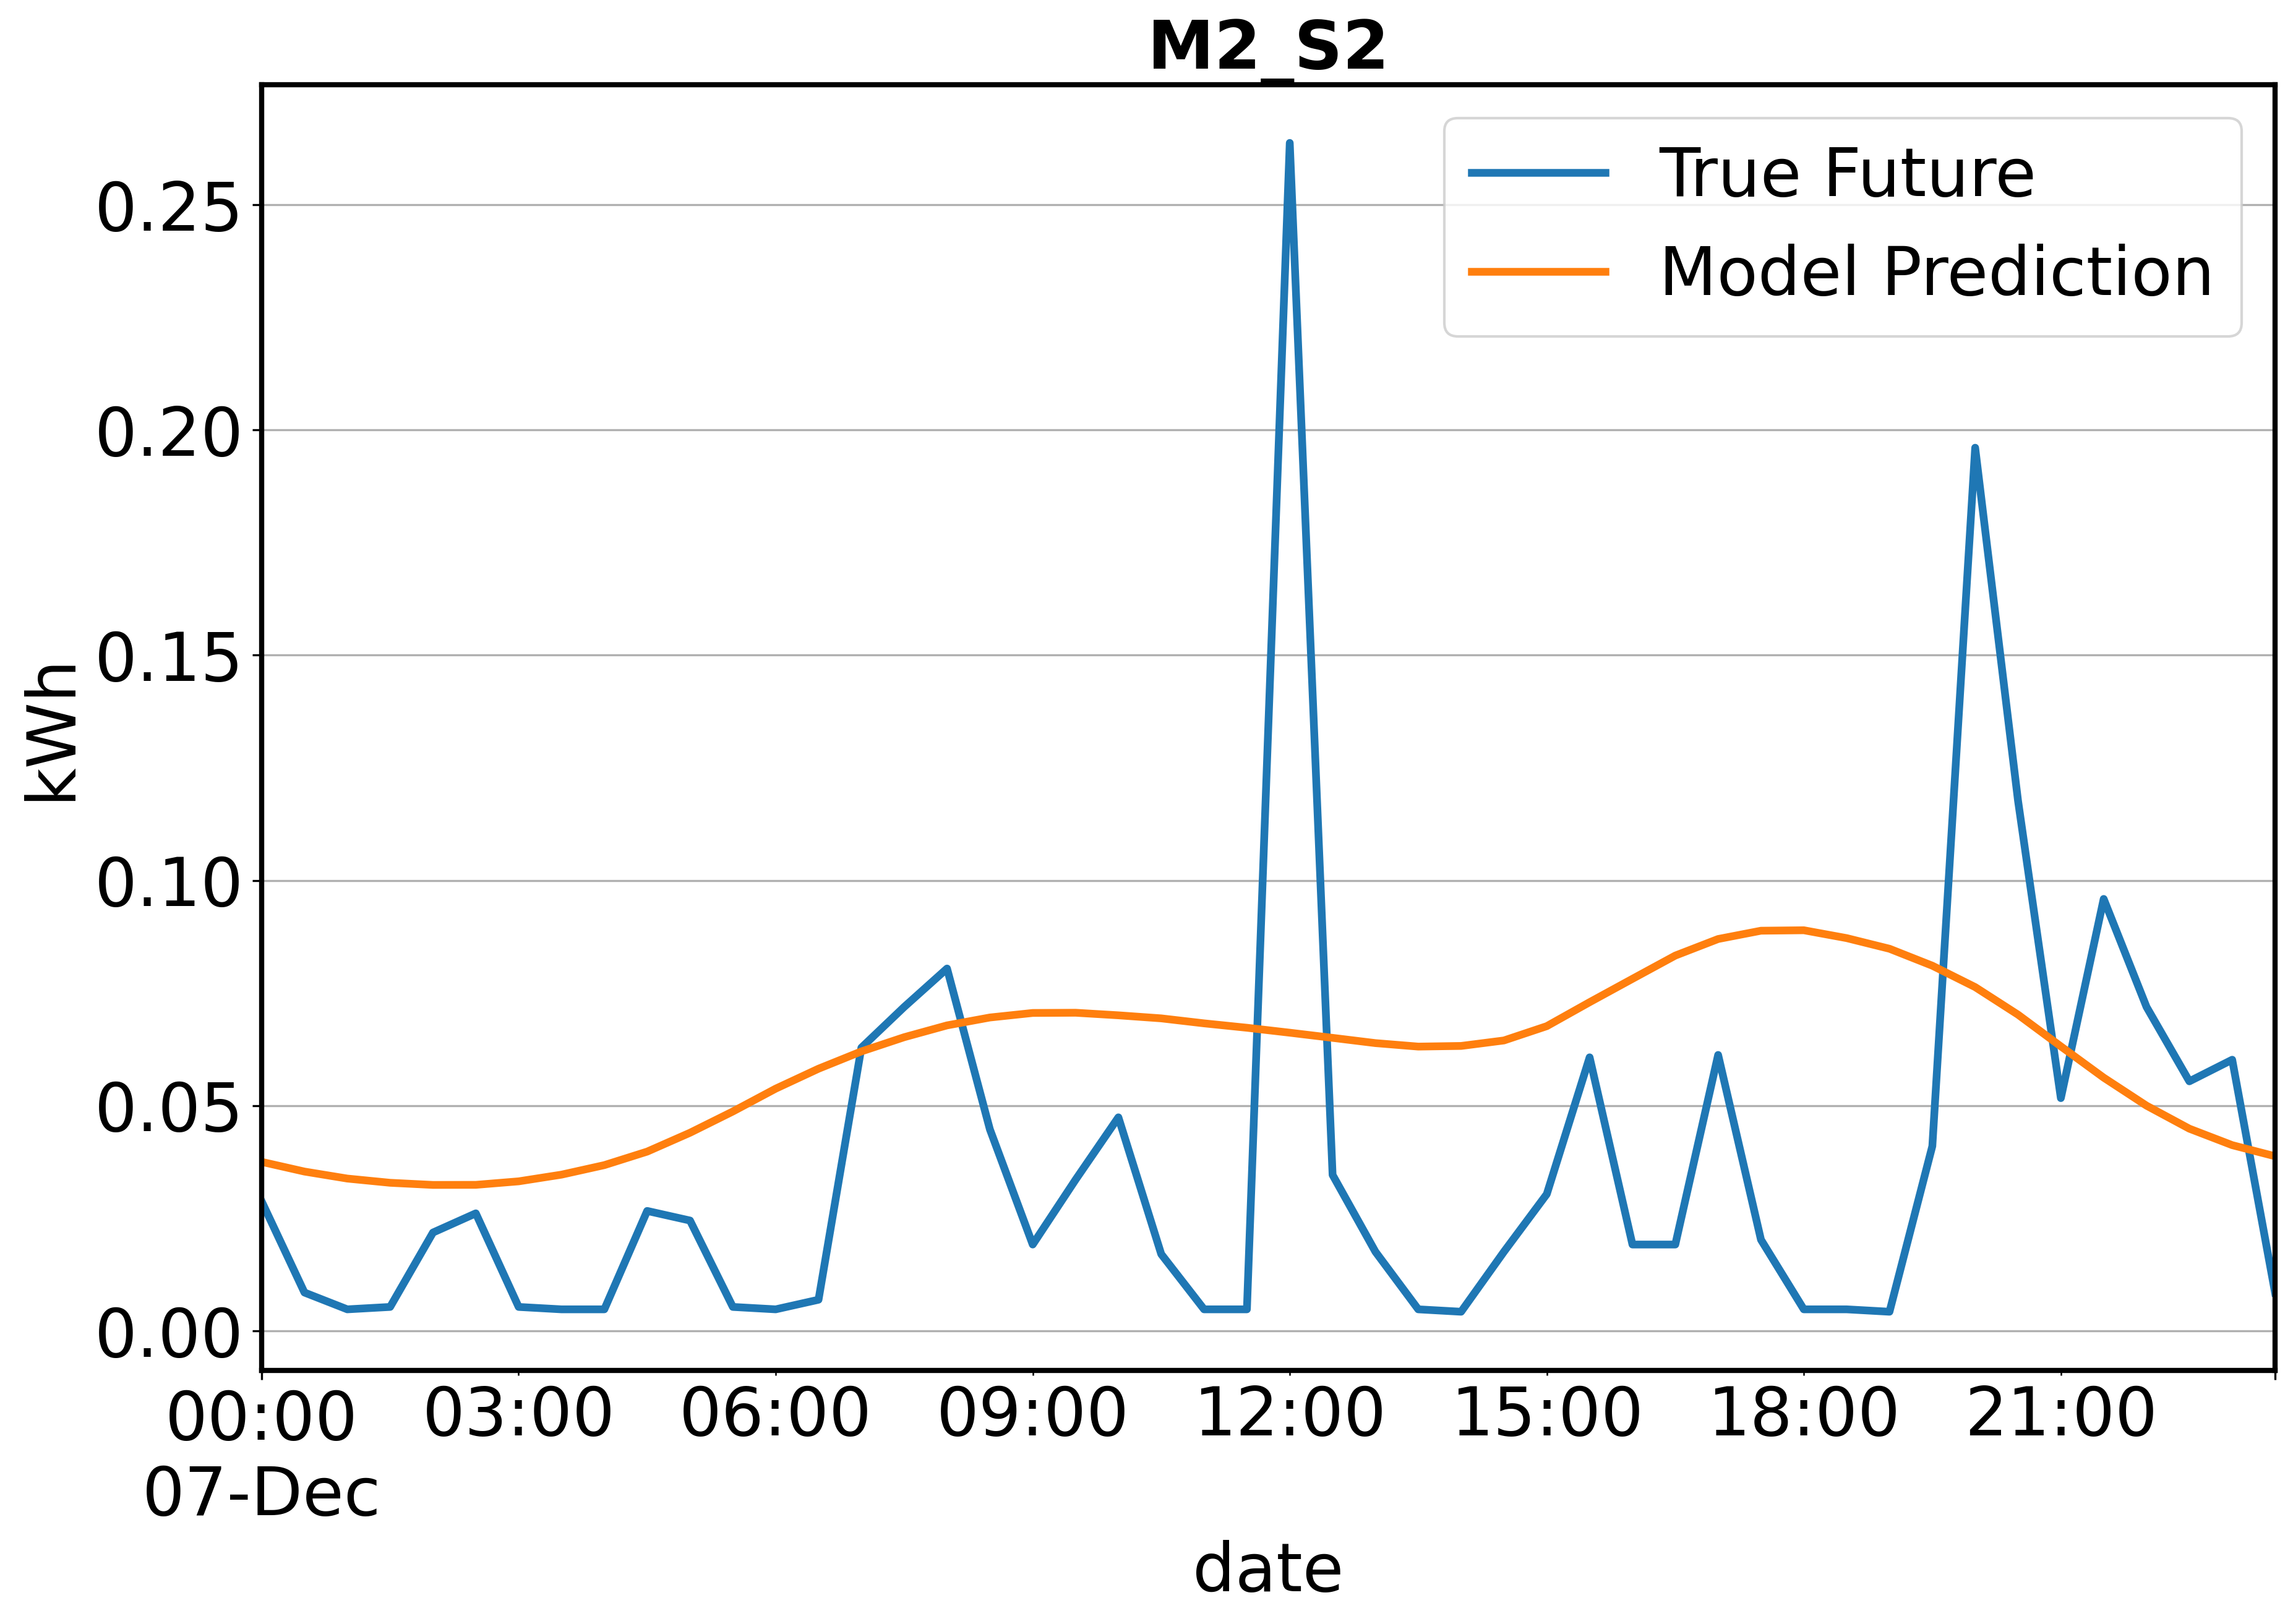
\includegraphics[width=1\linewidth]{IDM2_S2_Day341.png}
	 	\caption{Model $ 2 $ - Serie $ 2 $}
	 \end{subfigure}	
	 \begin{subfigure}{0.32\textwidth}
	 	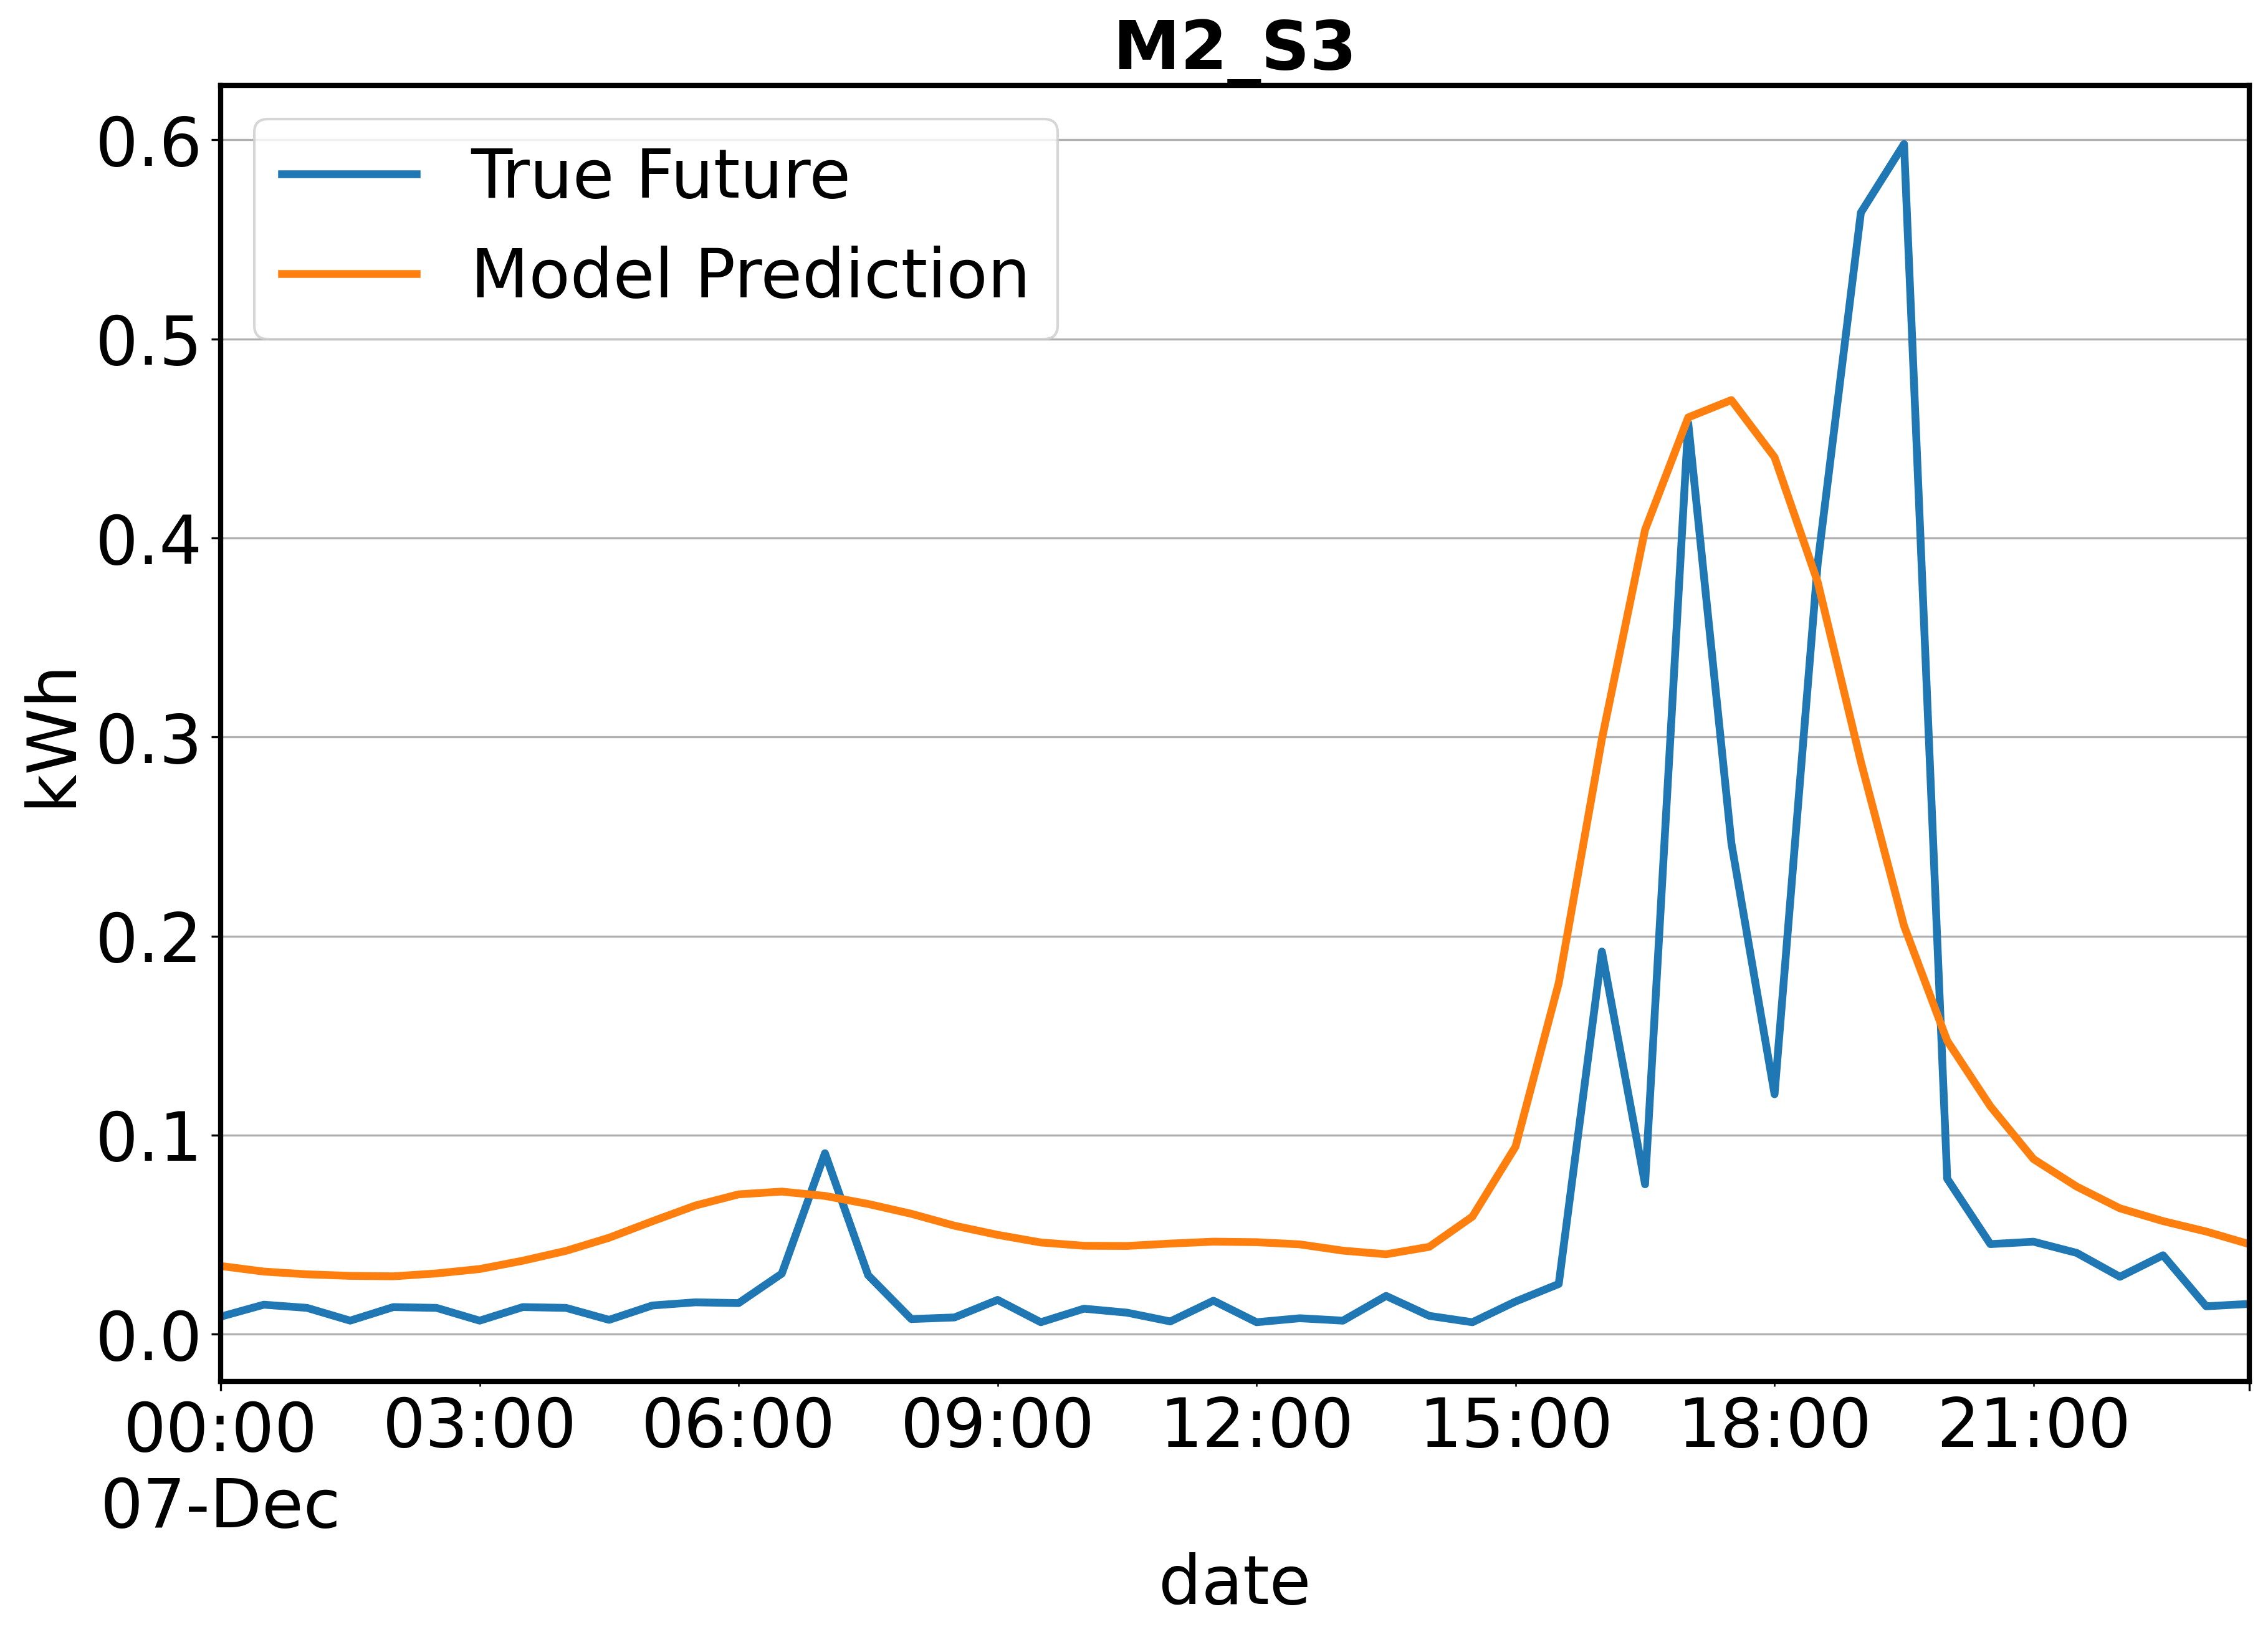
\includegraphics[width=1\linewidth]{IDM2_S3_Day341.png}
	 	\caption{Model $ 2 $ - Serie $ 3 $}
	 \end{subfigure}
 	\begin{subfigure}{0.32\textwidth}
	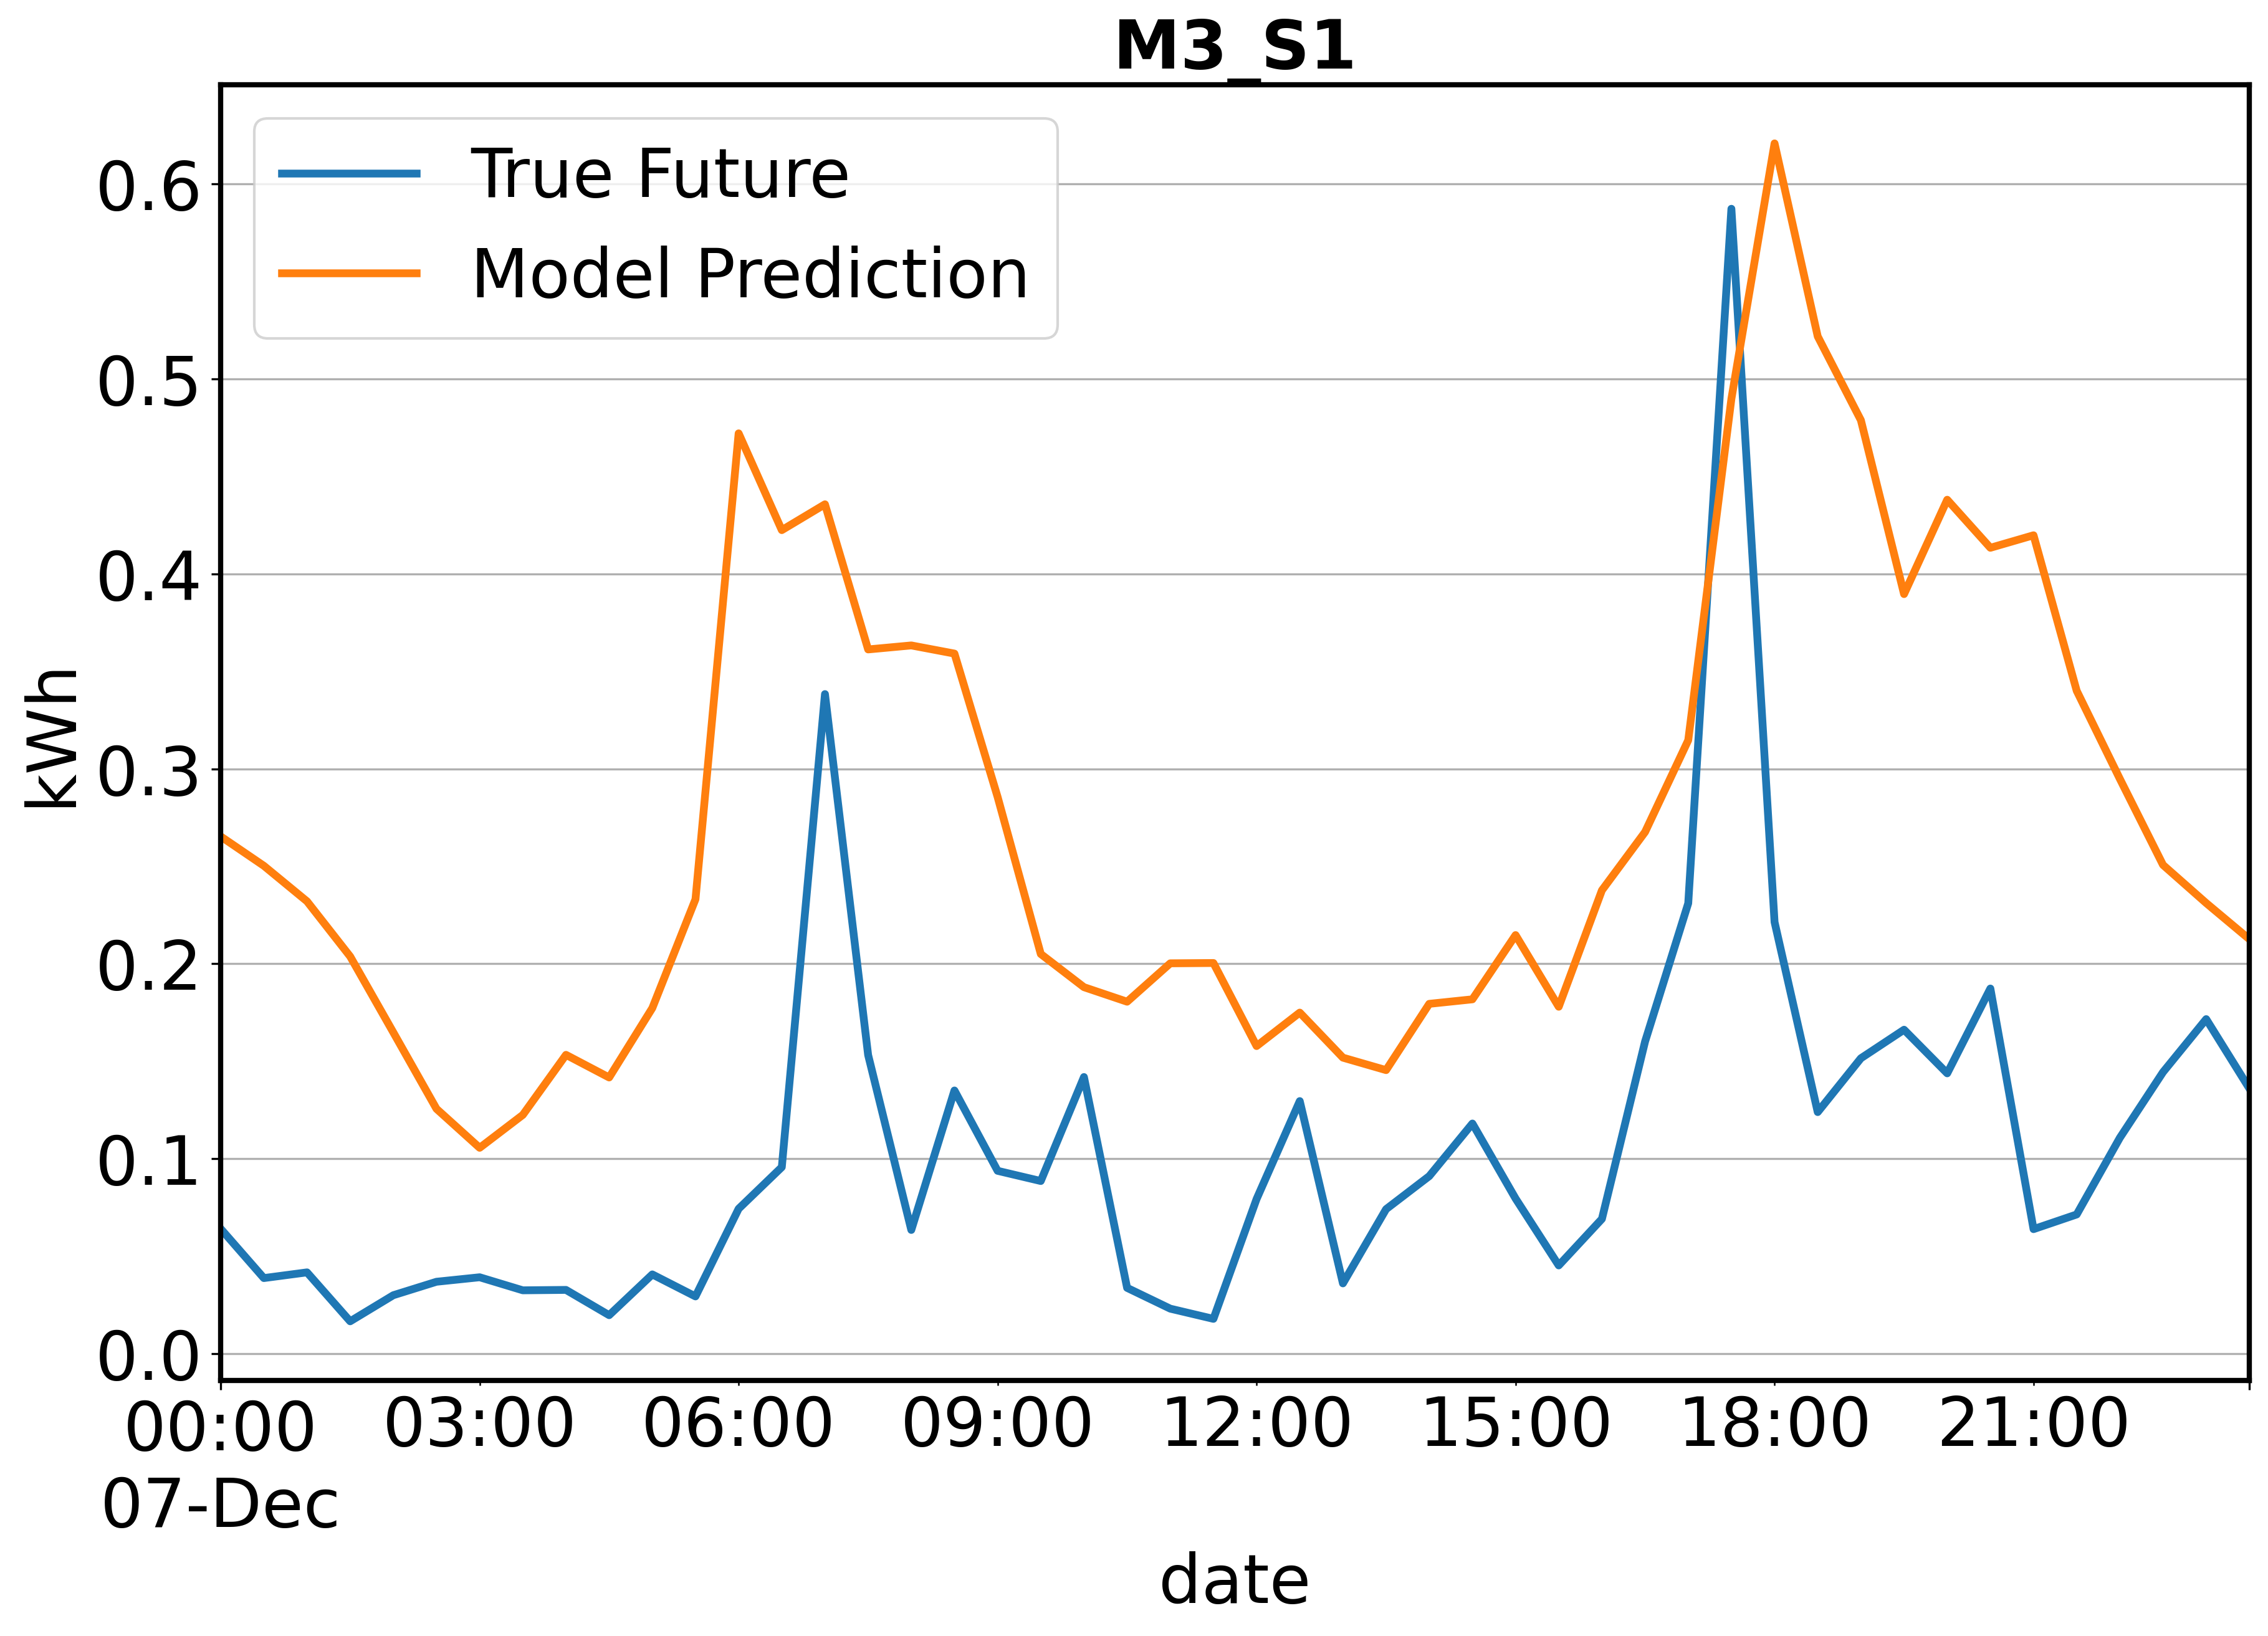
\includegraphics[width=1\linewidth]{IDM3_S1_Day341.png}
	\caption{Model $3 $ - Serie $ 1 $}
	\end{subfigure}	 	
	\begin{subfigure}{0.32\textwidth}
		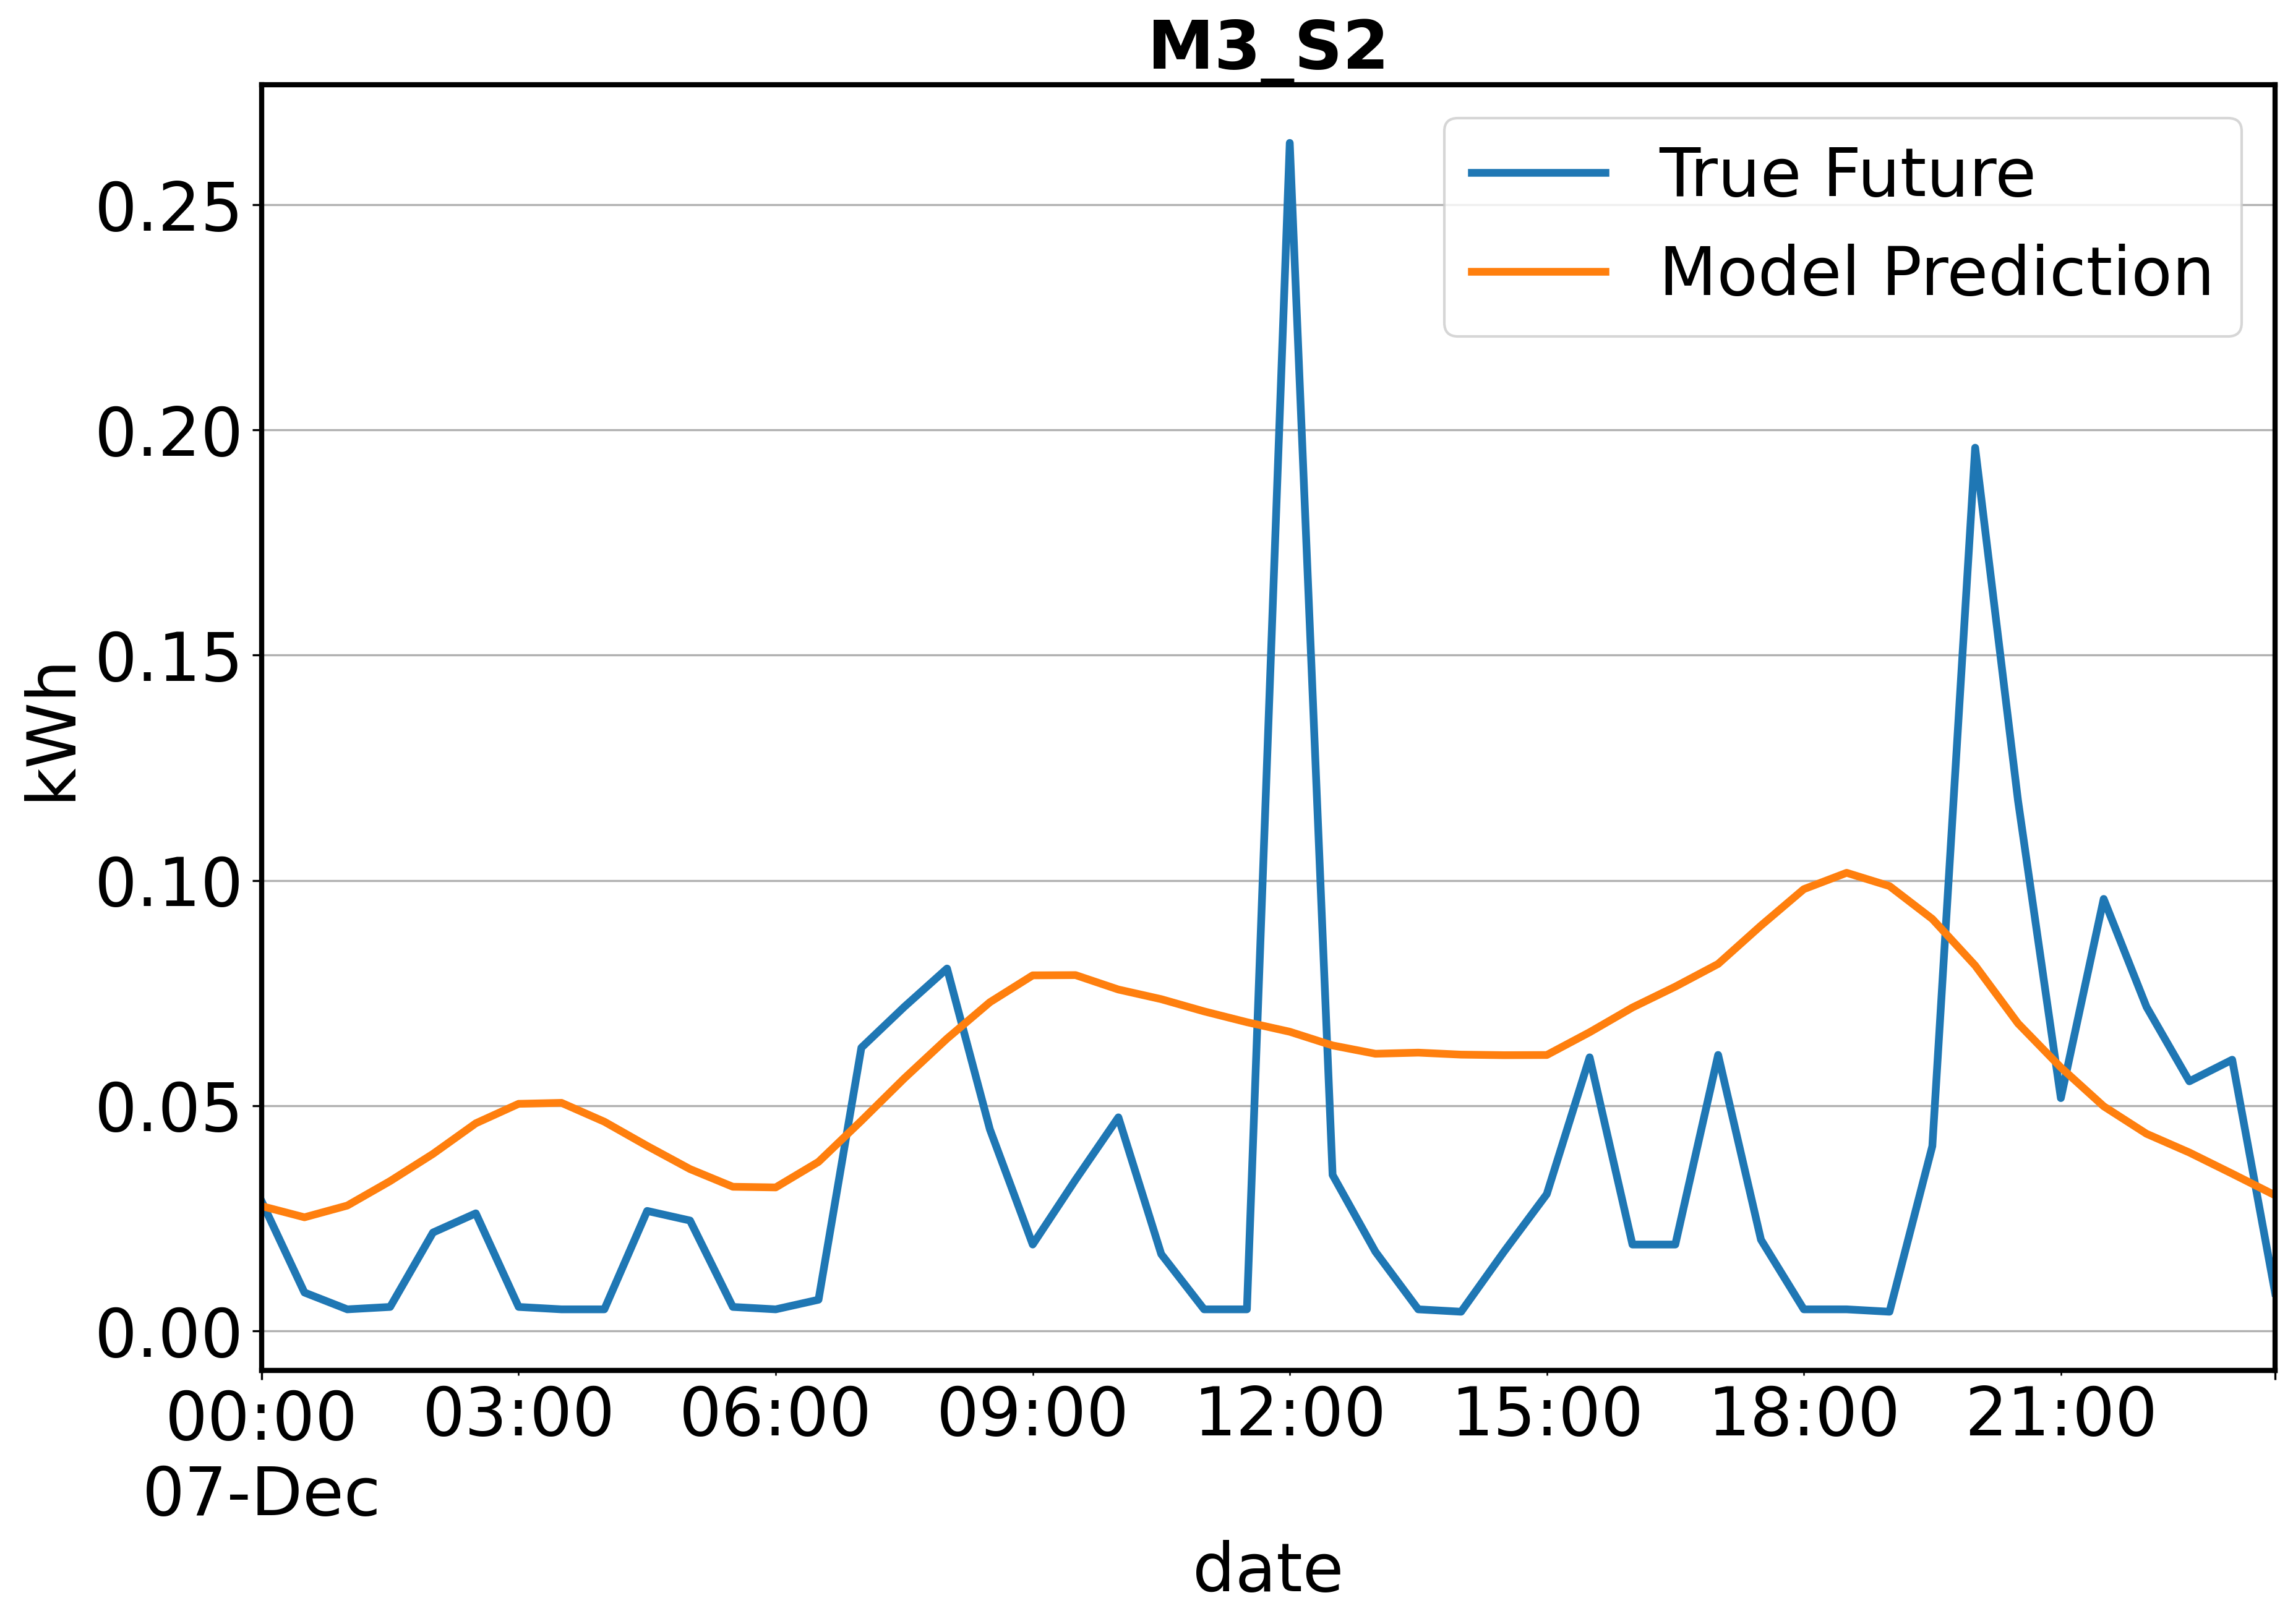
\includegraphics[width=1\linewidth]{IDM3_S2_Day341.png}
		\caption{Model $3 $ - Serie $ 2 $}
	\end{subfigure}	
	\begin{subfigure}{0.32\textwidth}
		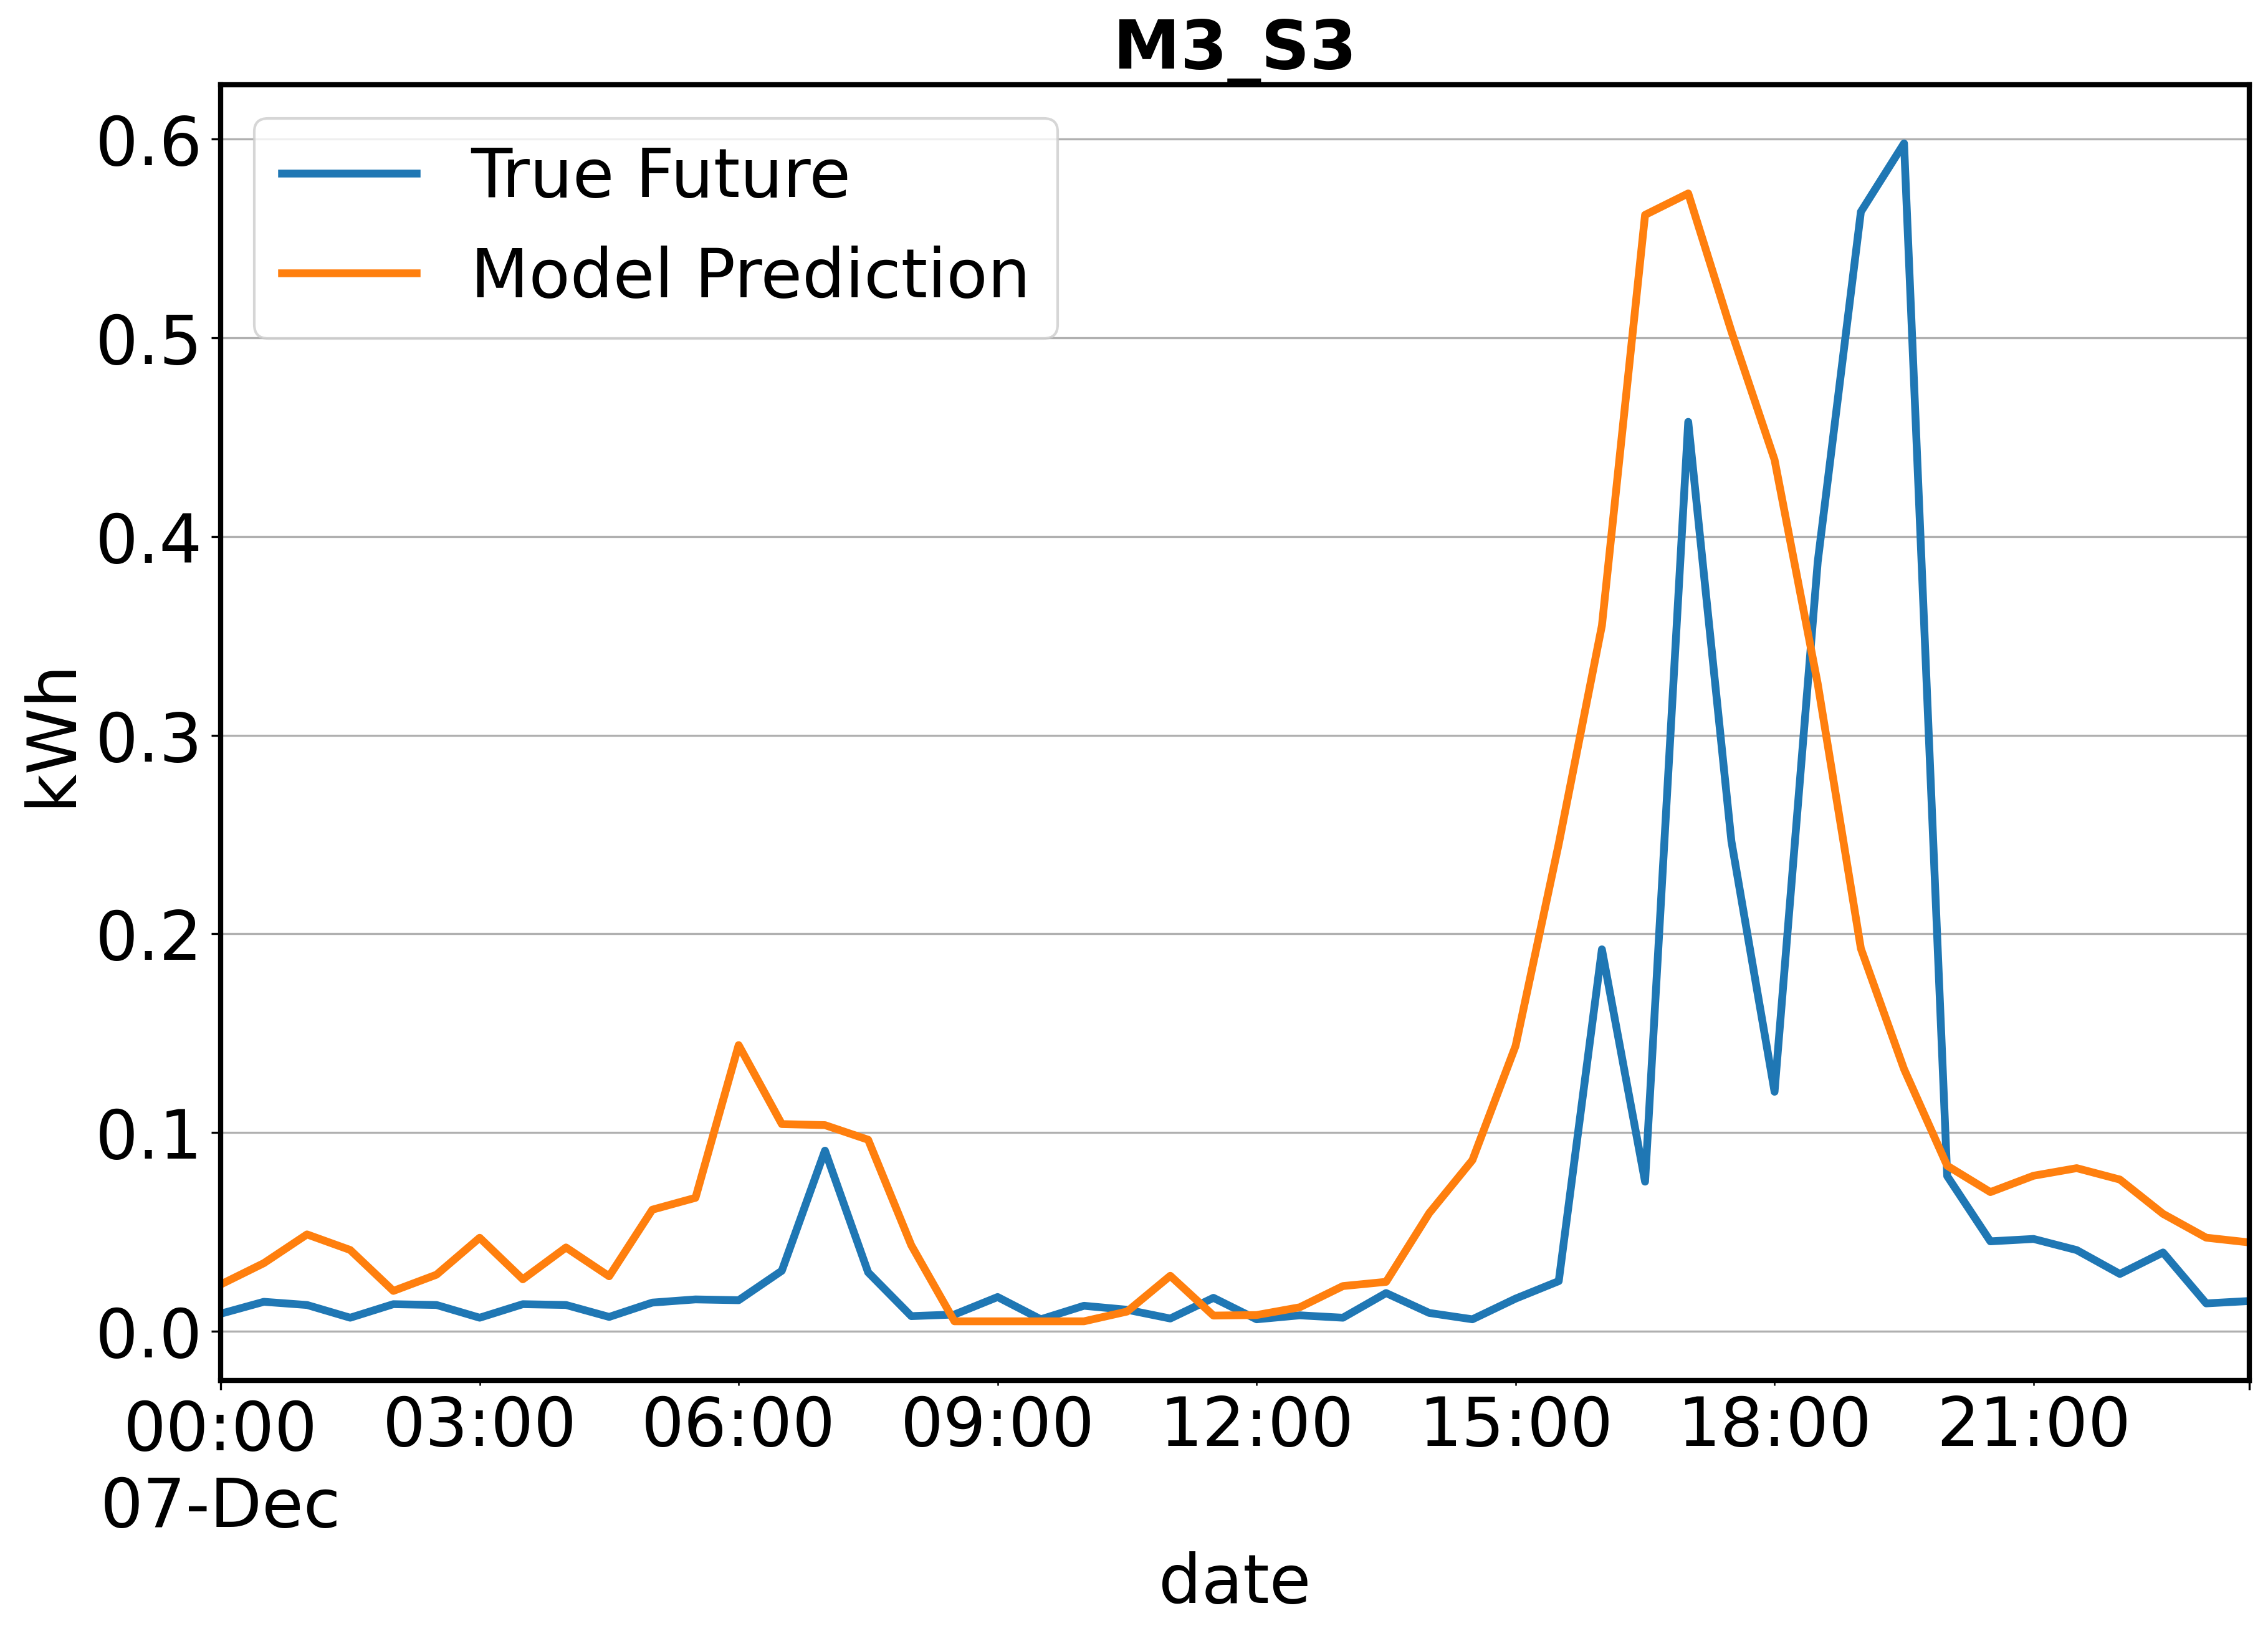
\includegraphics[width=1\linewidth]{IDM3_S3_Day341.png}
		\caption{Model $3 $ - Serie $ 3 $}
	\end{subfigure}
 	\begin{subfigure}{0.32\textwidth}
		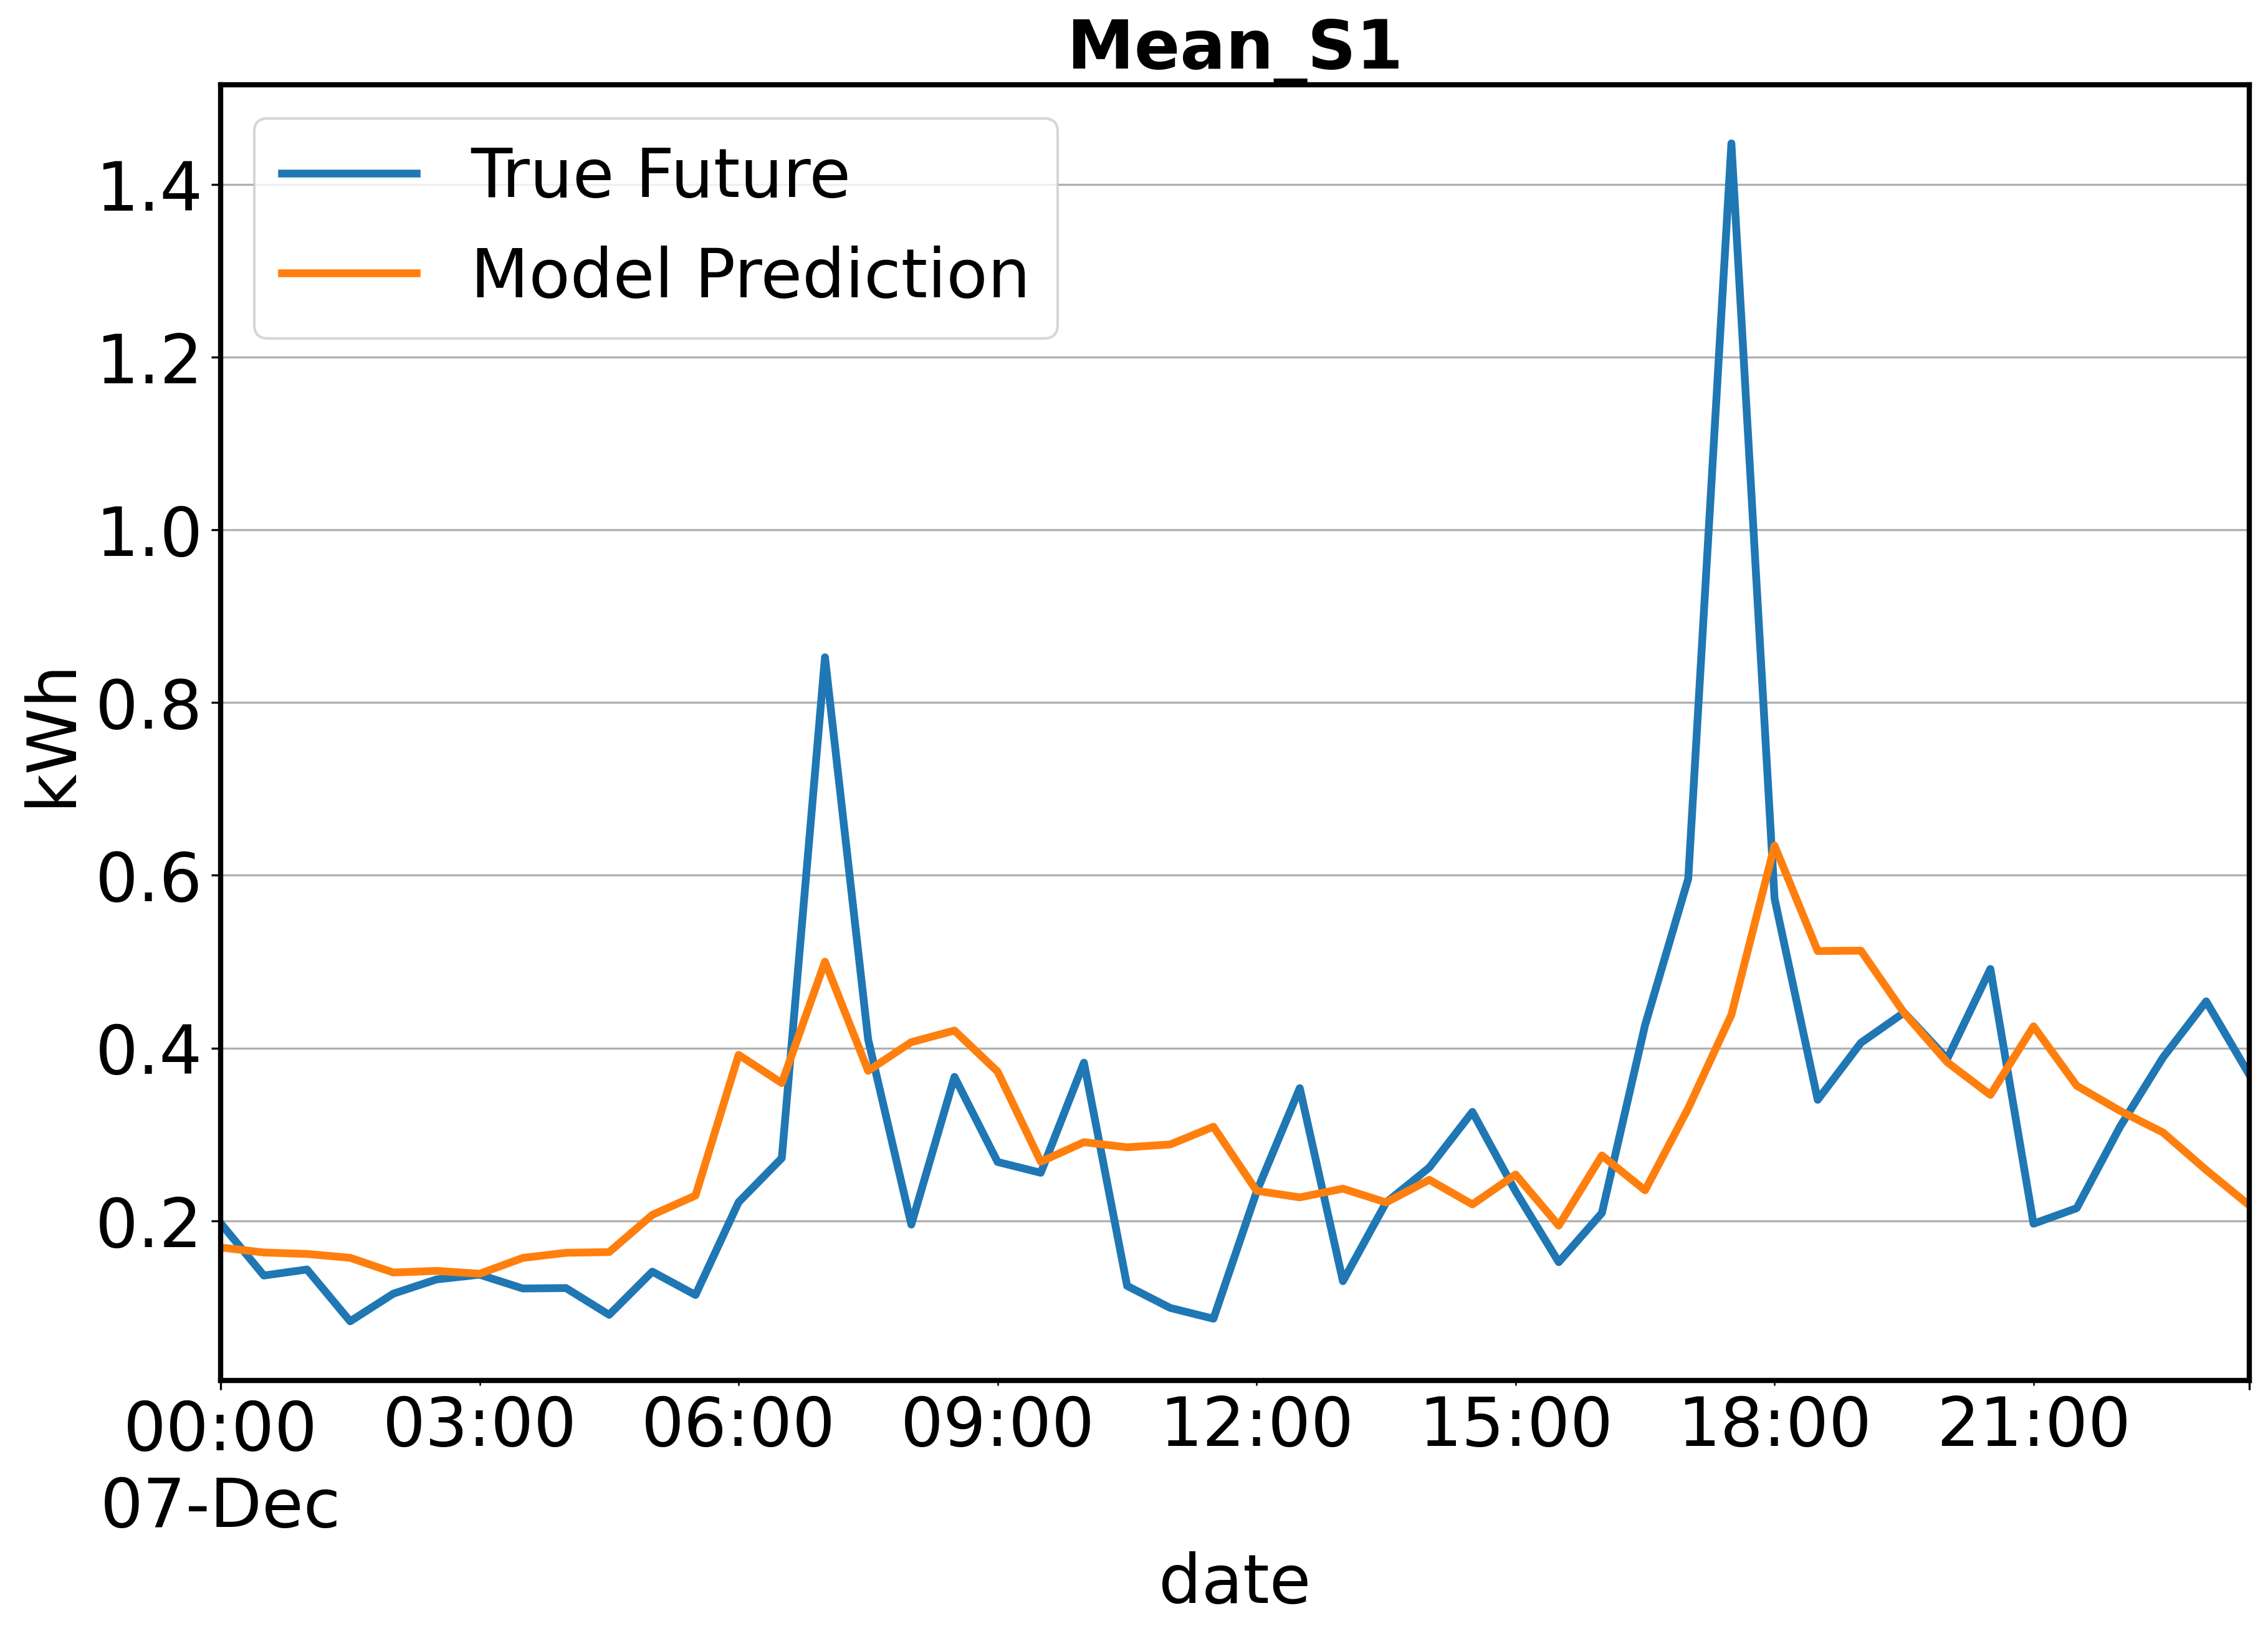
\includegraphics[width=1\linewidth]{IDMean_S1_Day341.png}
		\caption{Mean forecast - Serie $ 1 $}
	\end{subfigure}	 	
	\begin{subfigure}{0.32\textwidth}
		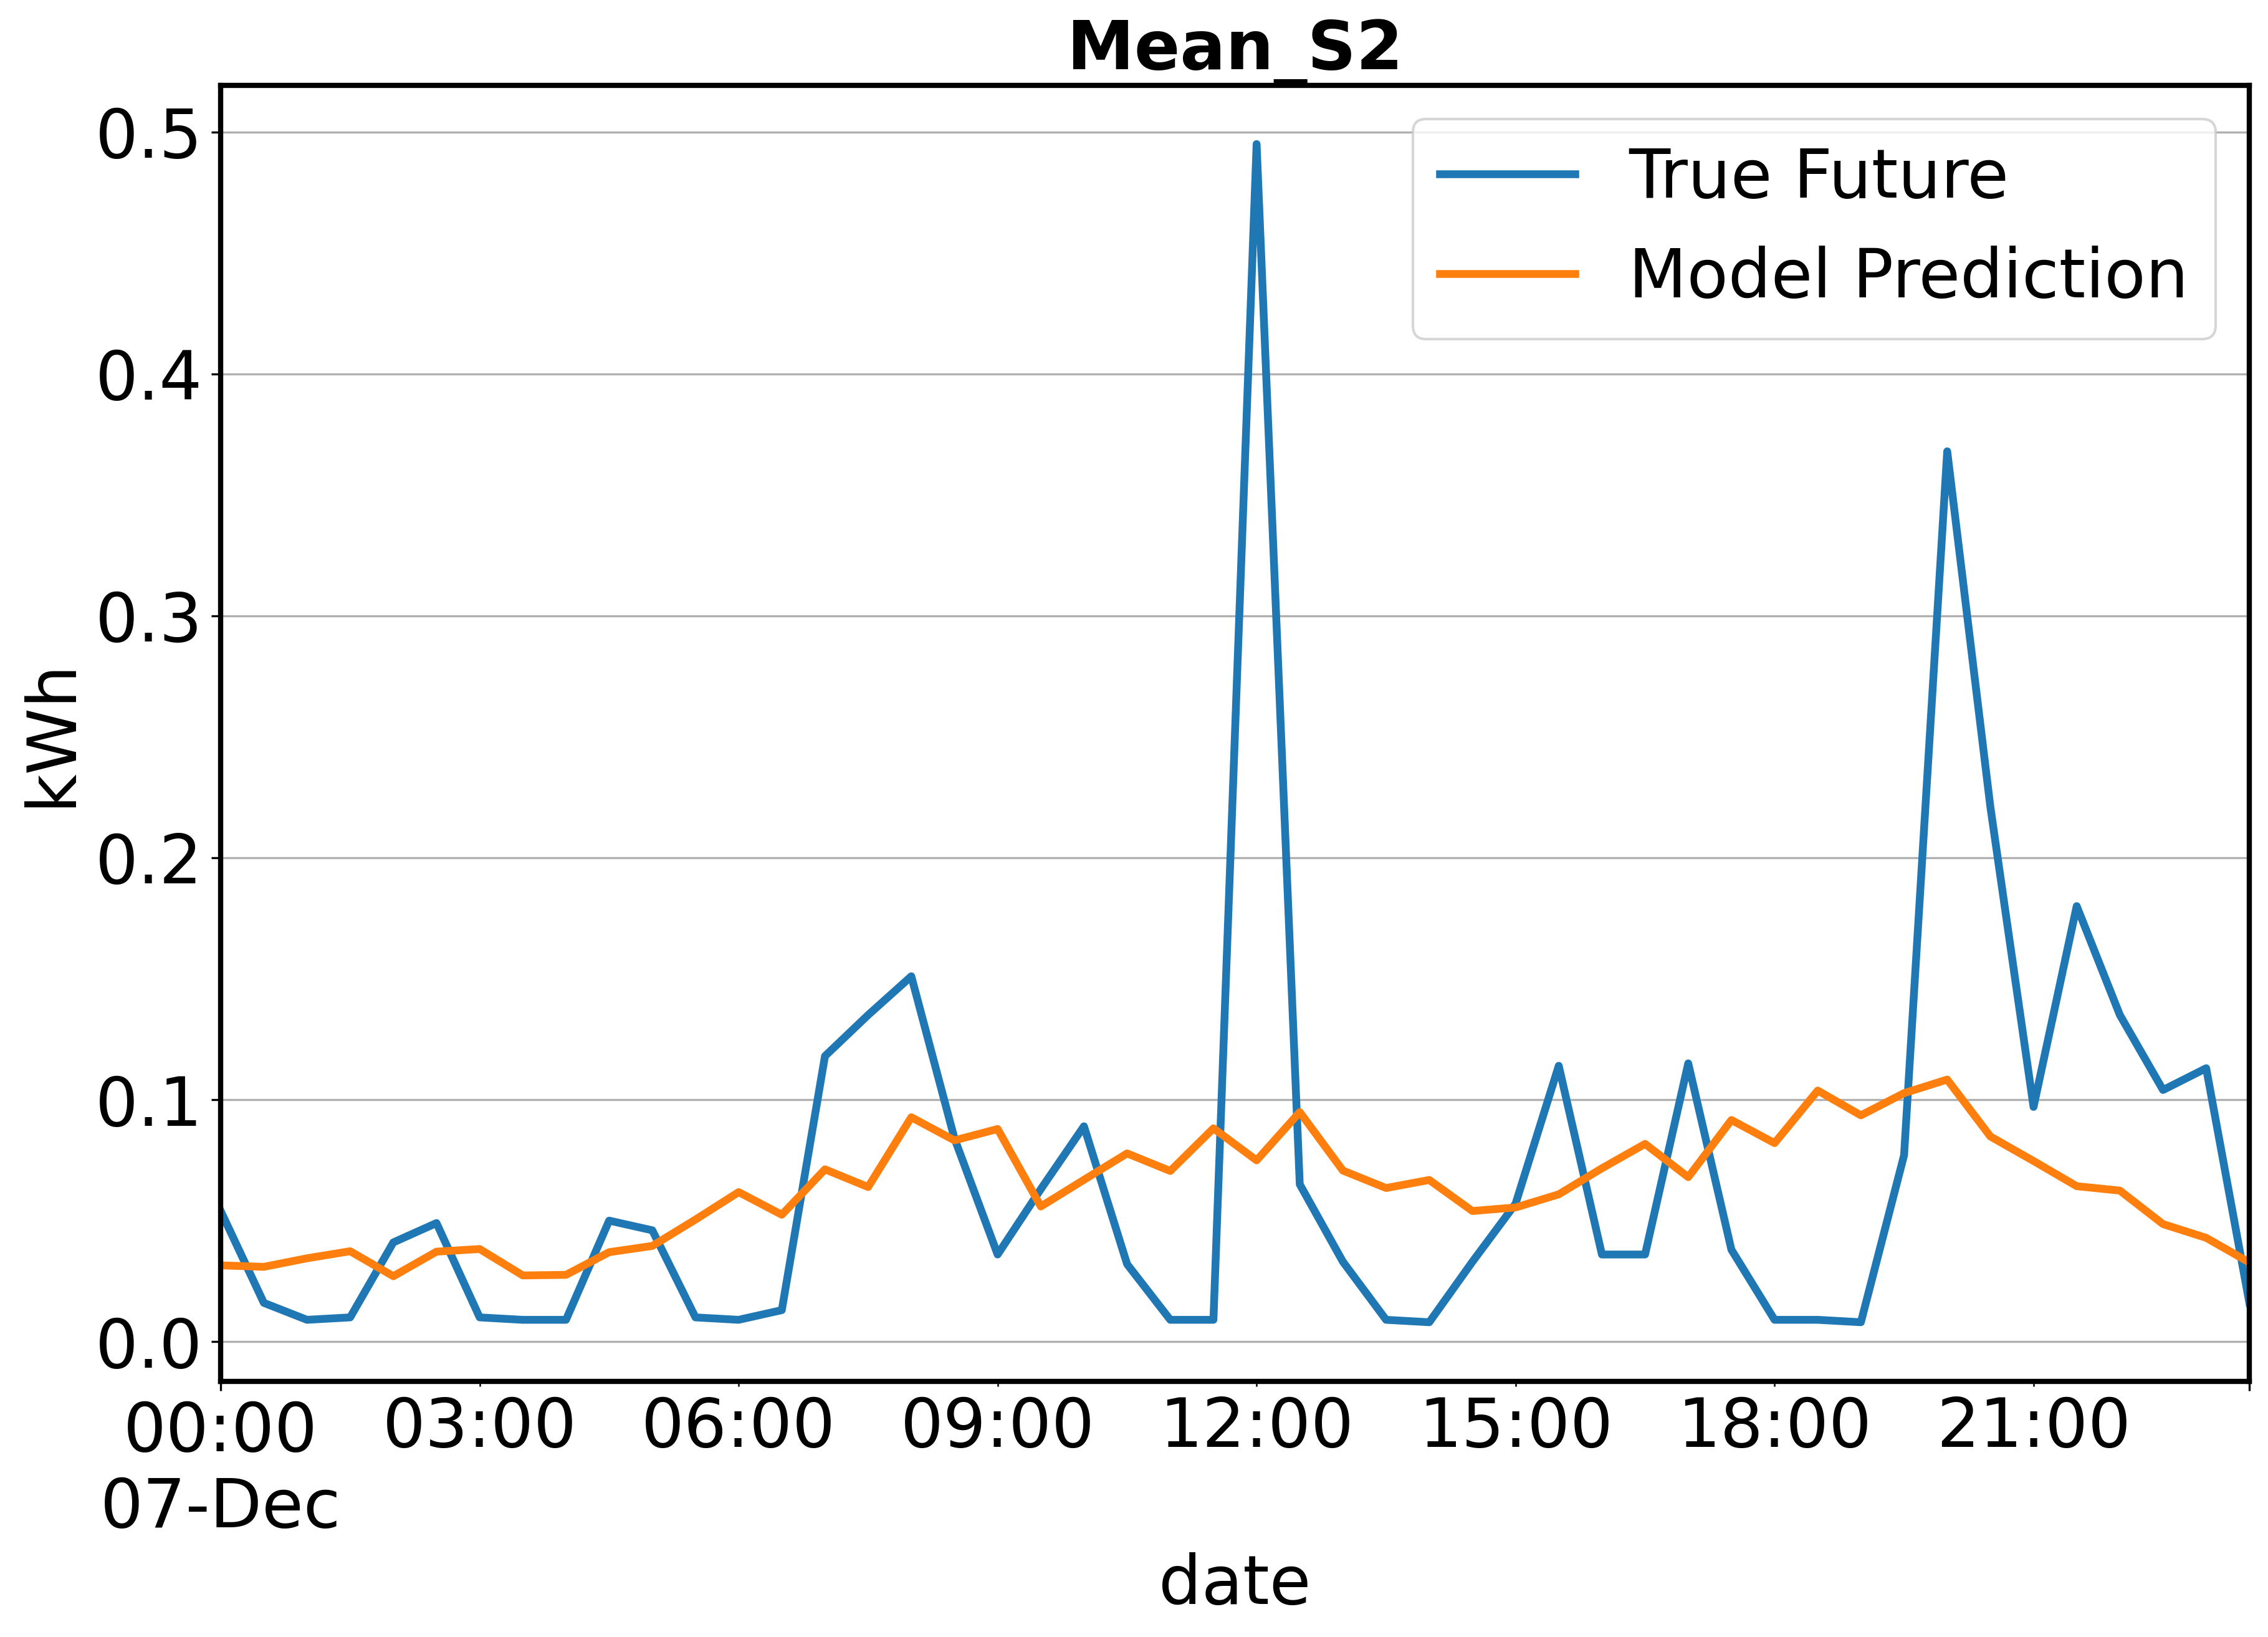
\includegraphics[width=1\linewidth]{IDMean_S2_Day341.png}
		\caption{Mean forecast - Serie $ 2 $}
	\end{subfigure}	
	\begin{subfigure}{0.32\textwidth}
		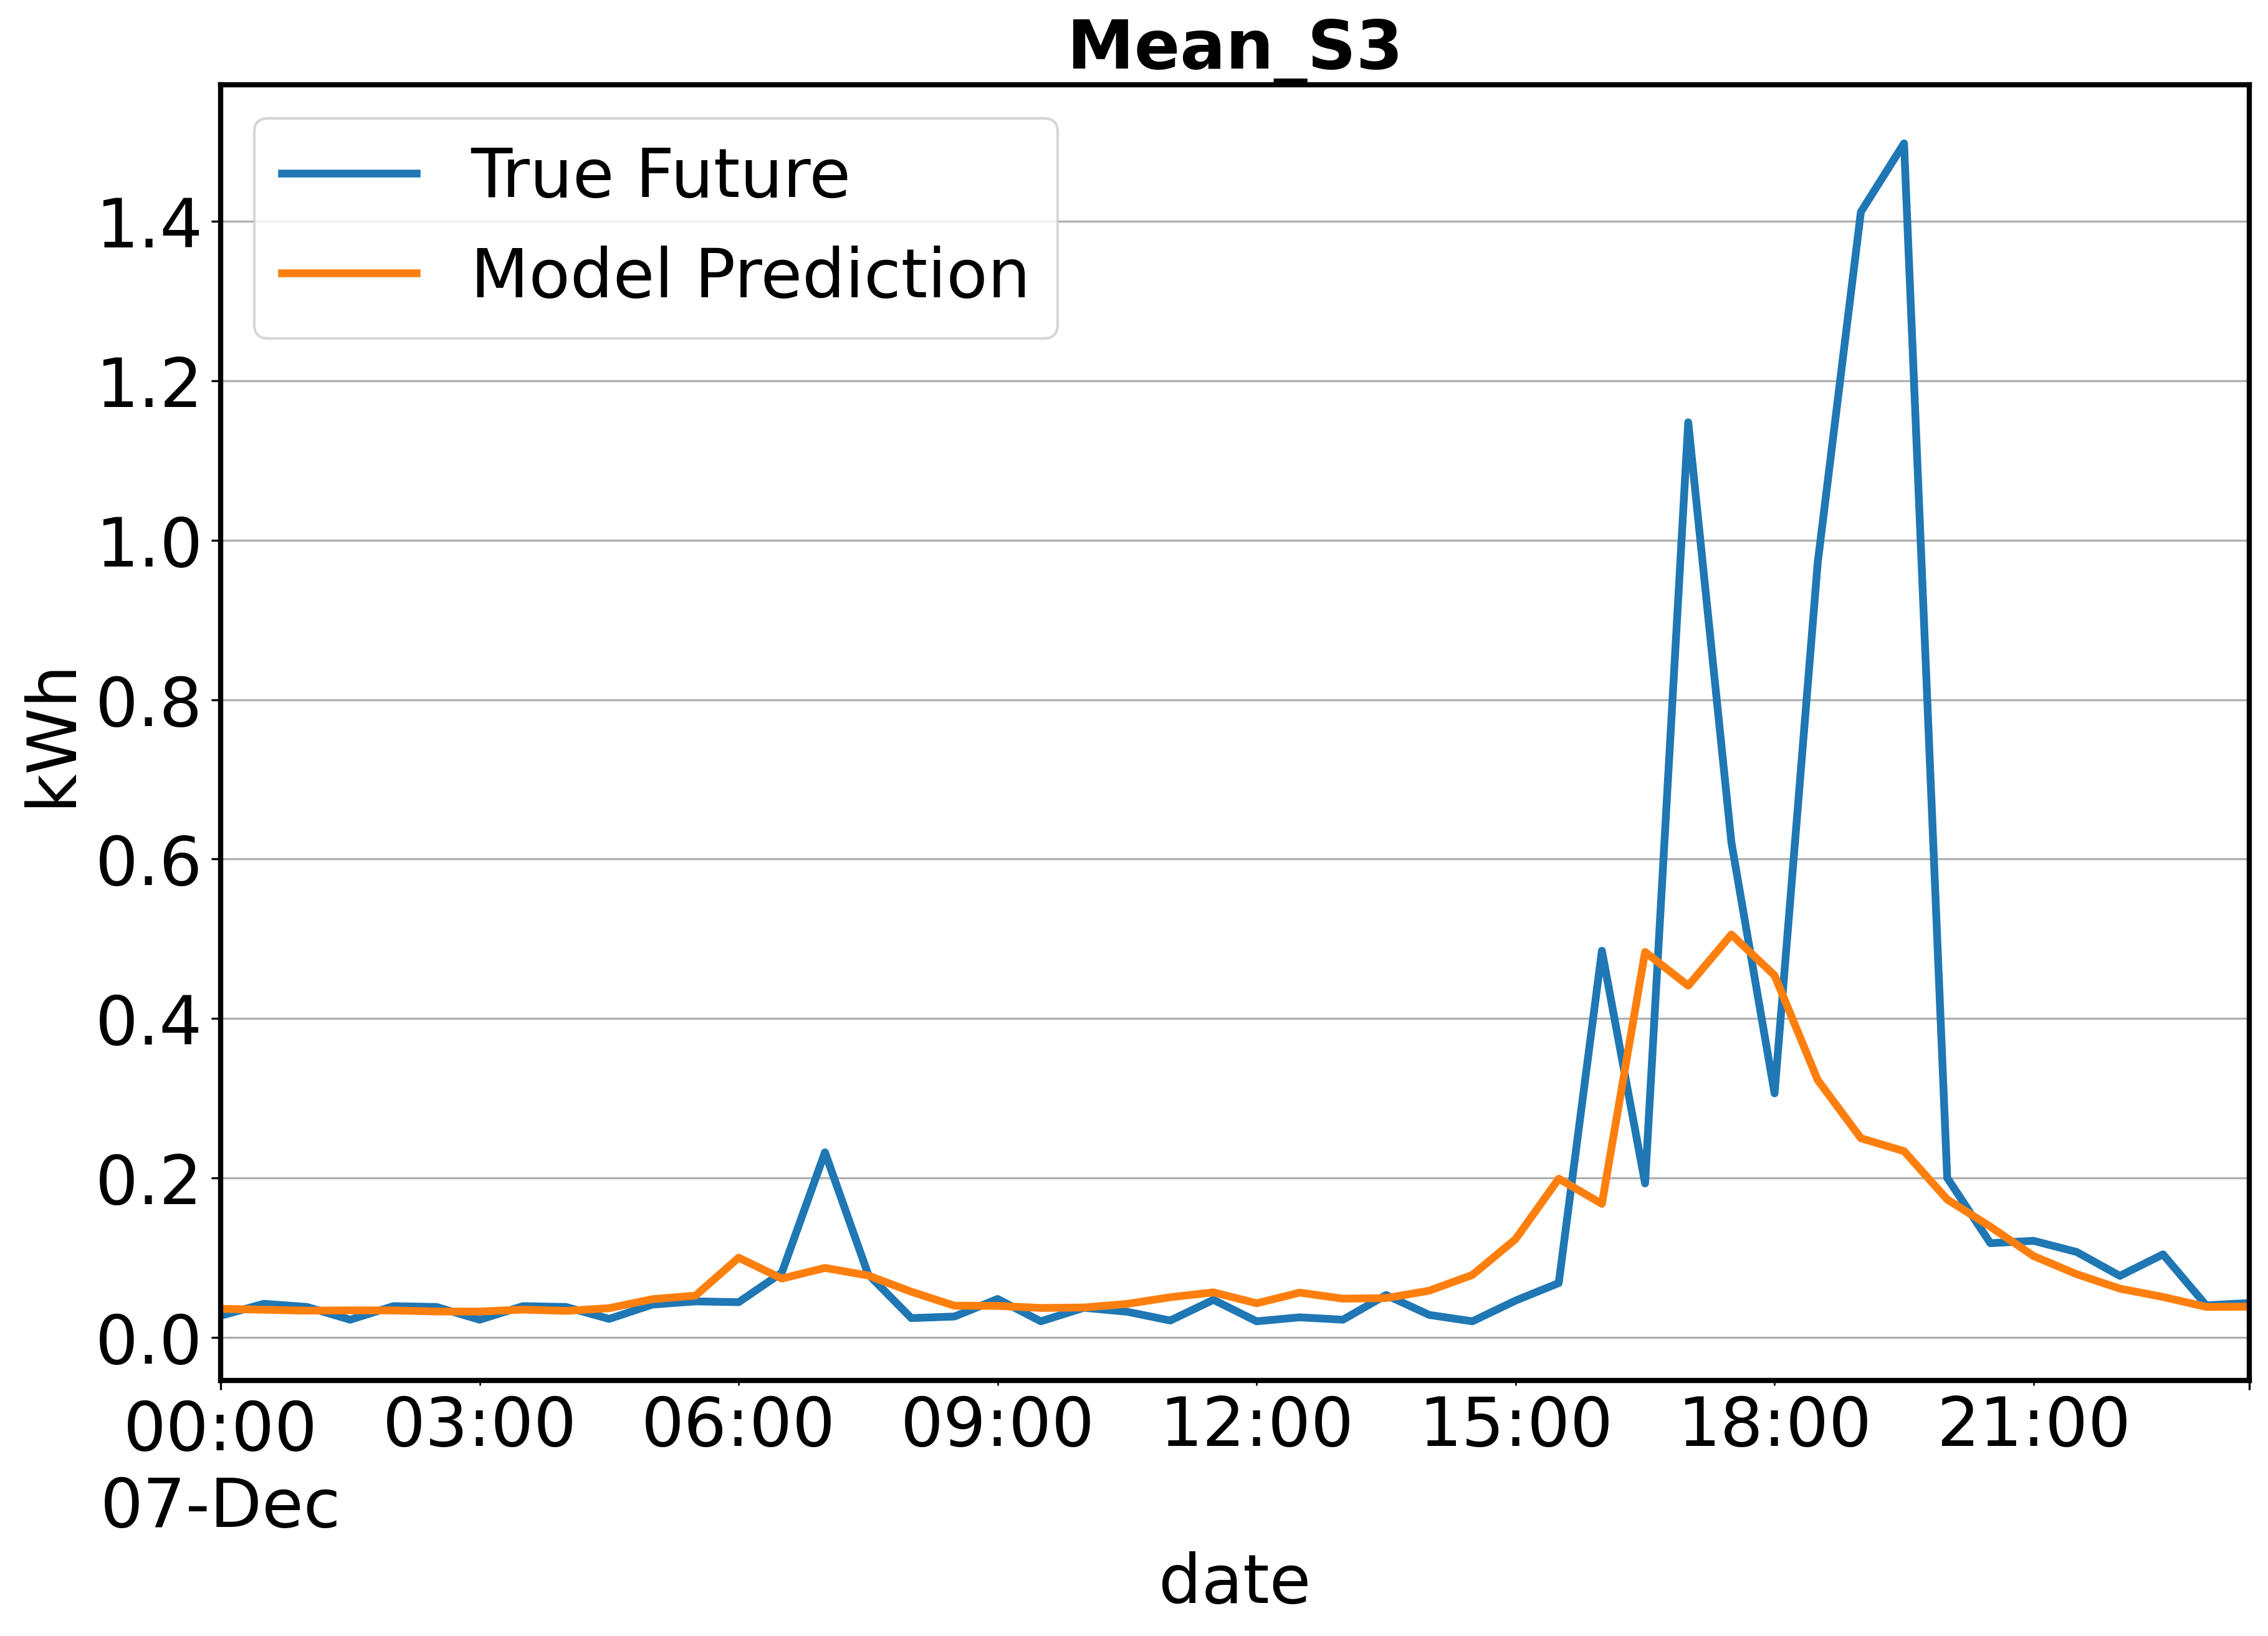
\includegraphics[width=1\linewidth]{IDMean_S3_Day341.png}
		\caption{Mean forecast - Serie $ 3 $}
	\end{subfigure}
	 \begin{subfigure}{0.32\textwidth}
		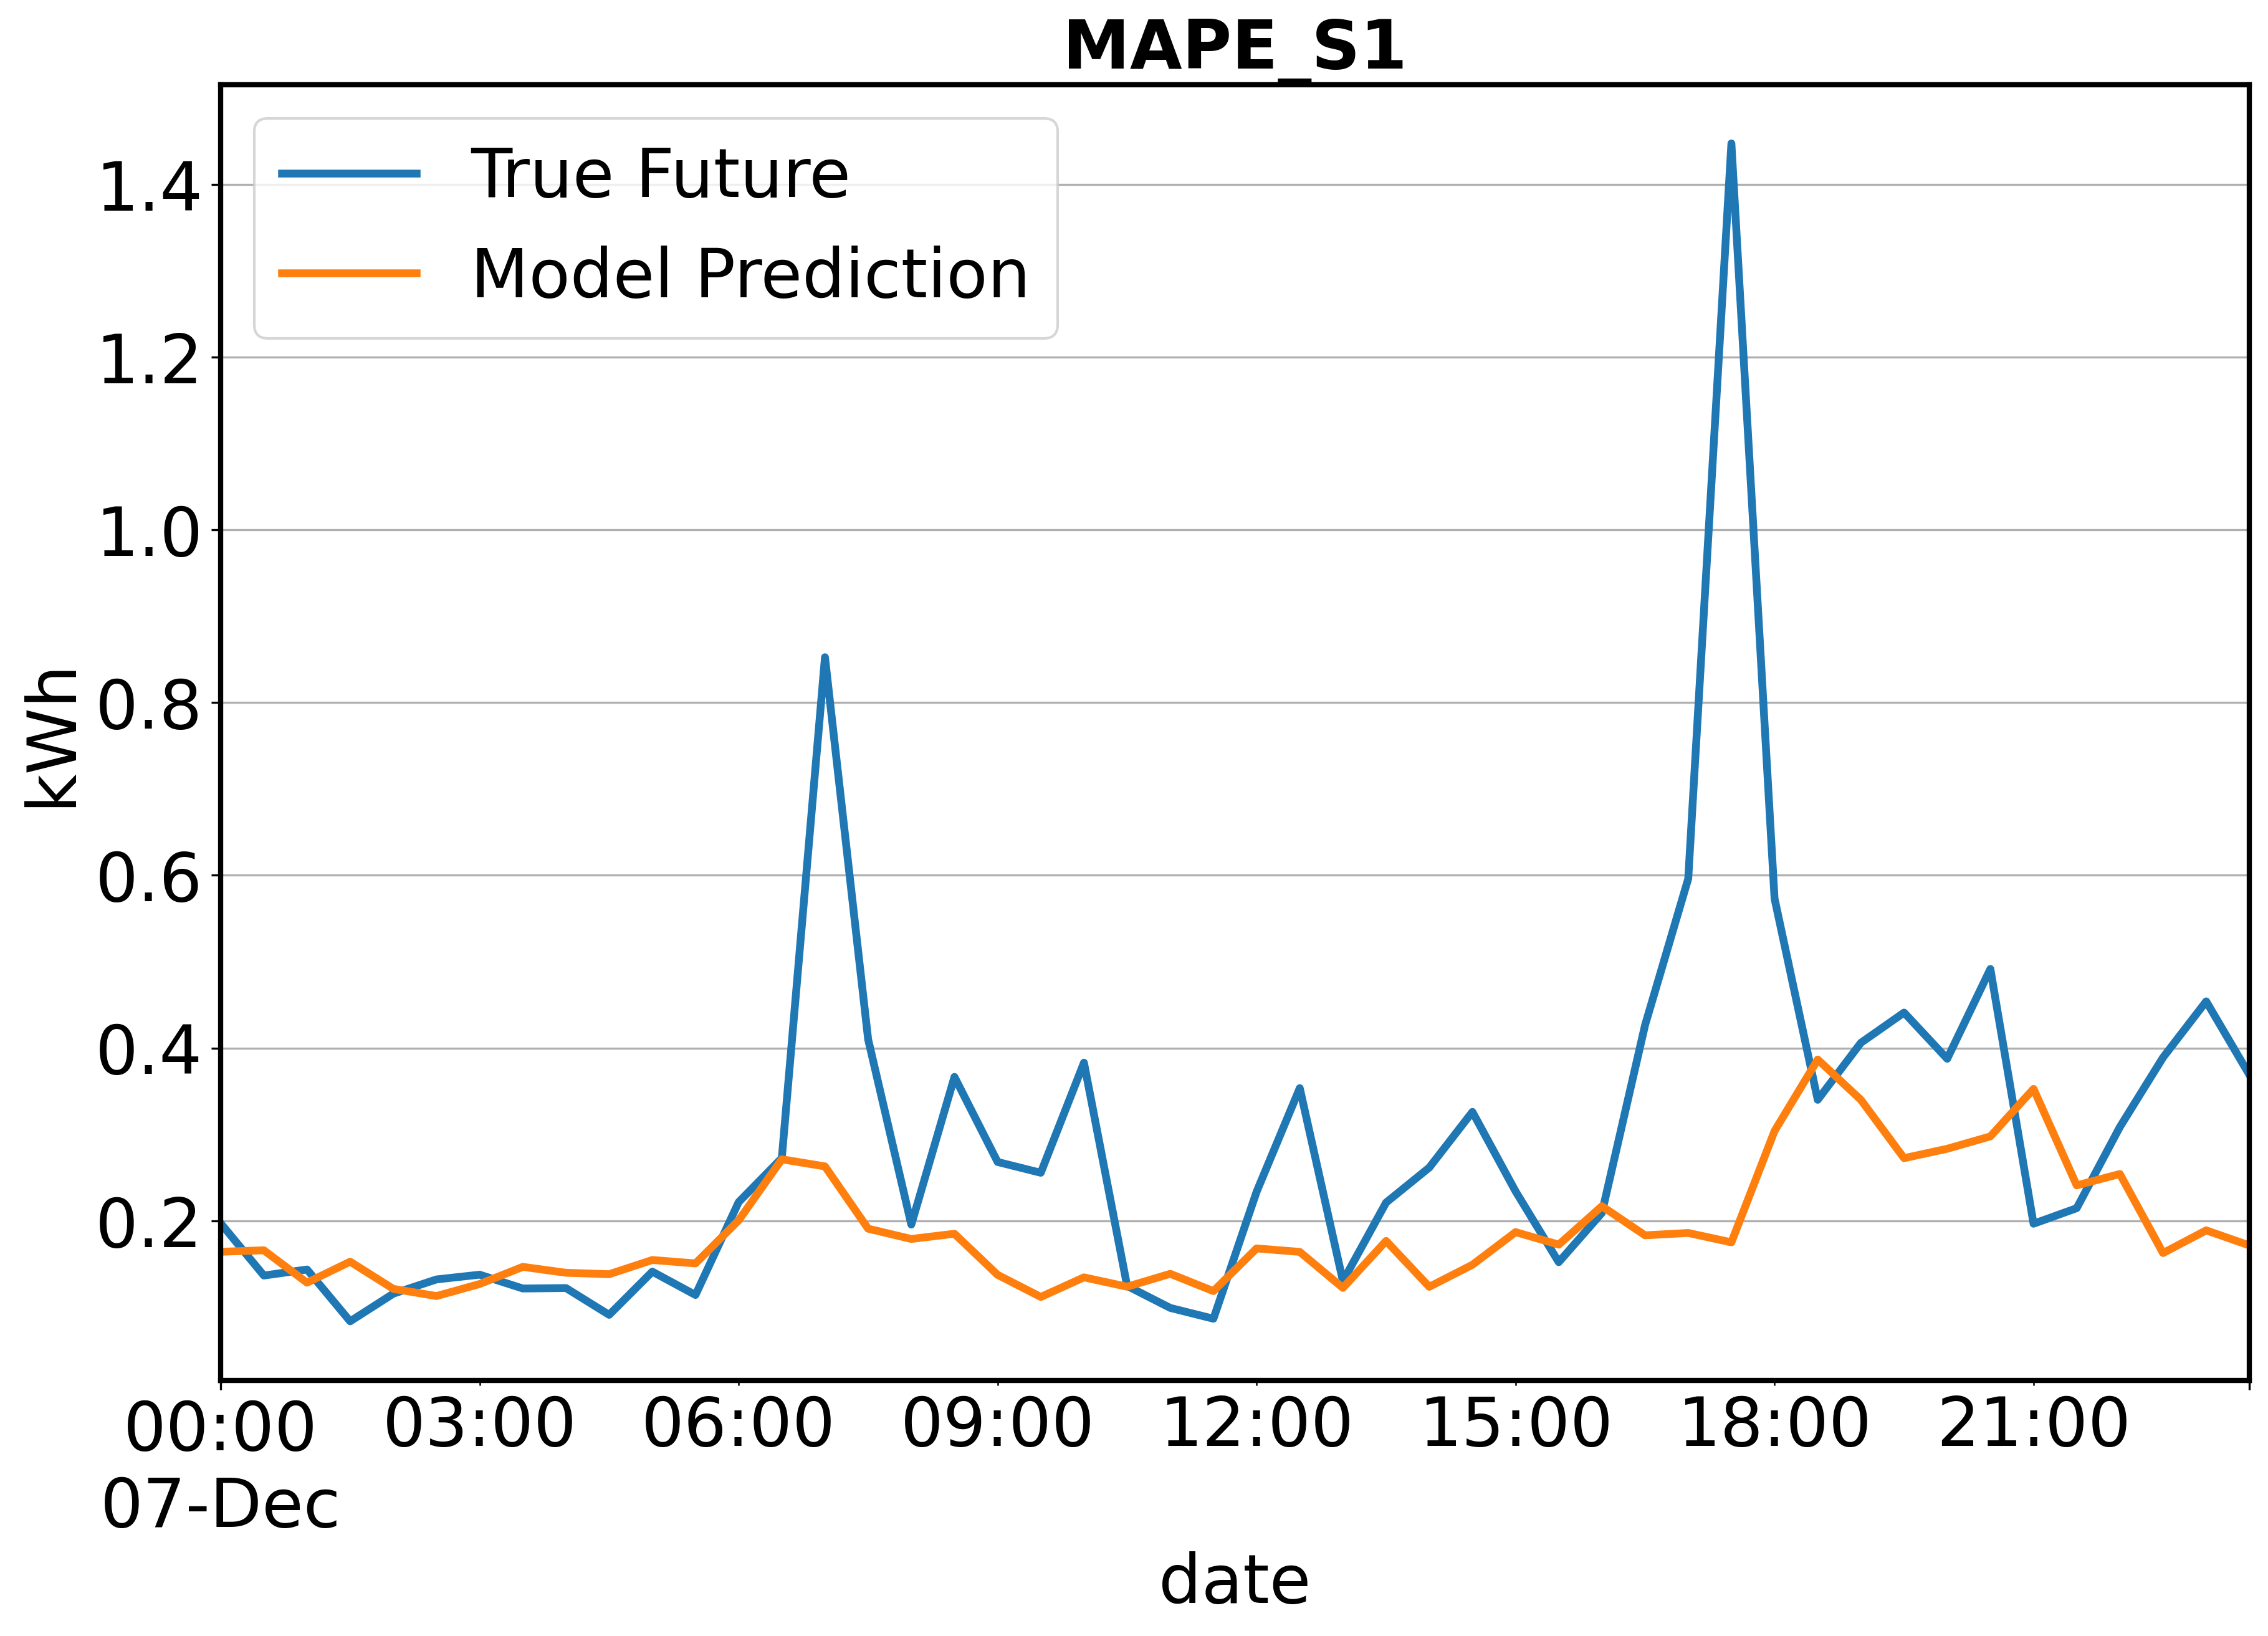
\includegraphics[width=1\linewidth]{IDMAPE_S1_Day341.png}
		\caption{MAPE forecast - Serie $ 1 $}
	\end{subfigure}	 	
	\begin{subfigure}{0.32\textwidth}
		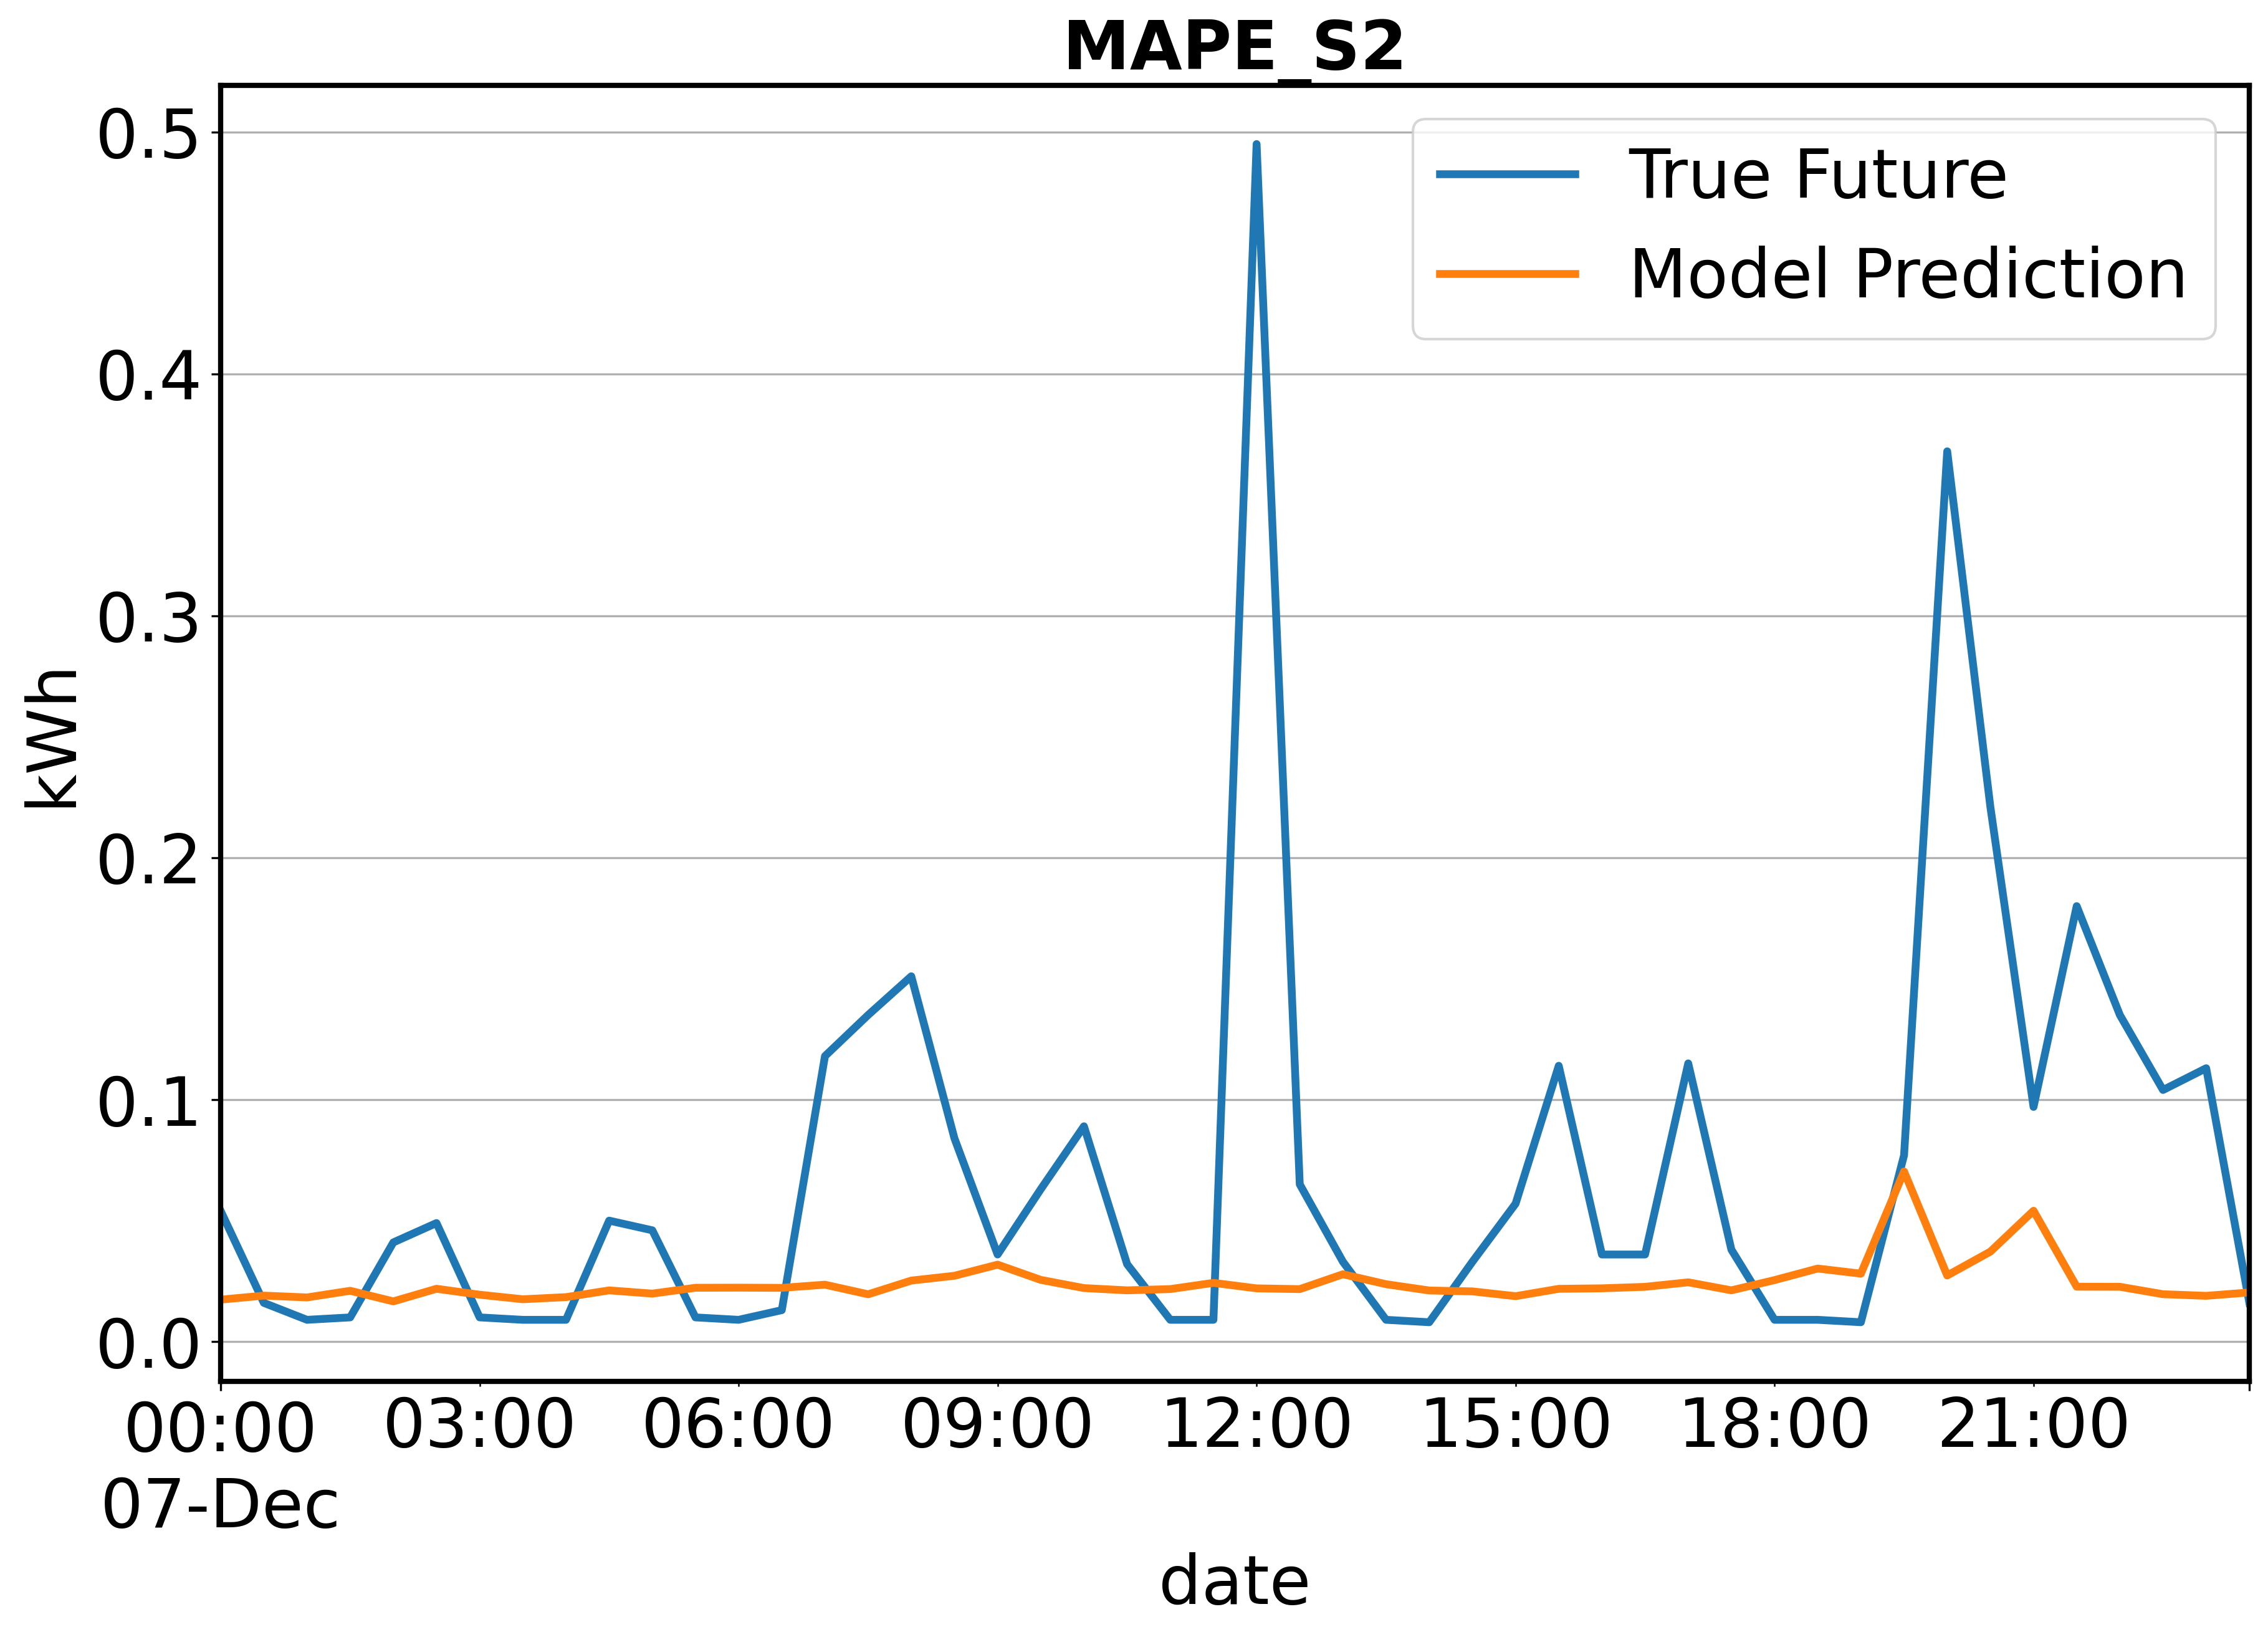
\includegraphics[width=1\linewidth]{IDMAPE_S2_Day341.png}
		\caption{MAPE forecast - Serie $ 2 $}
	\end{subfigure}	
	\begin{subfigure}{0.32\textwidth}
		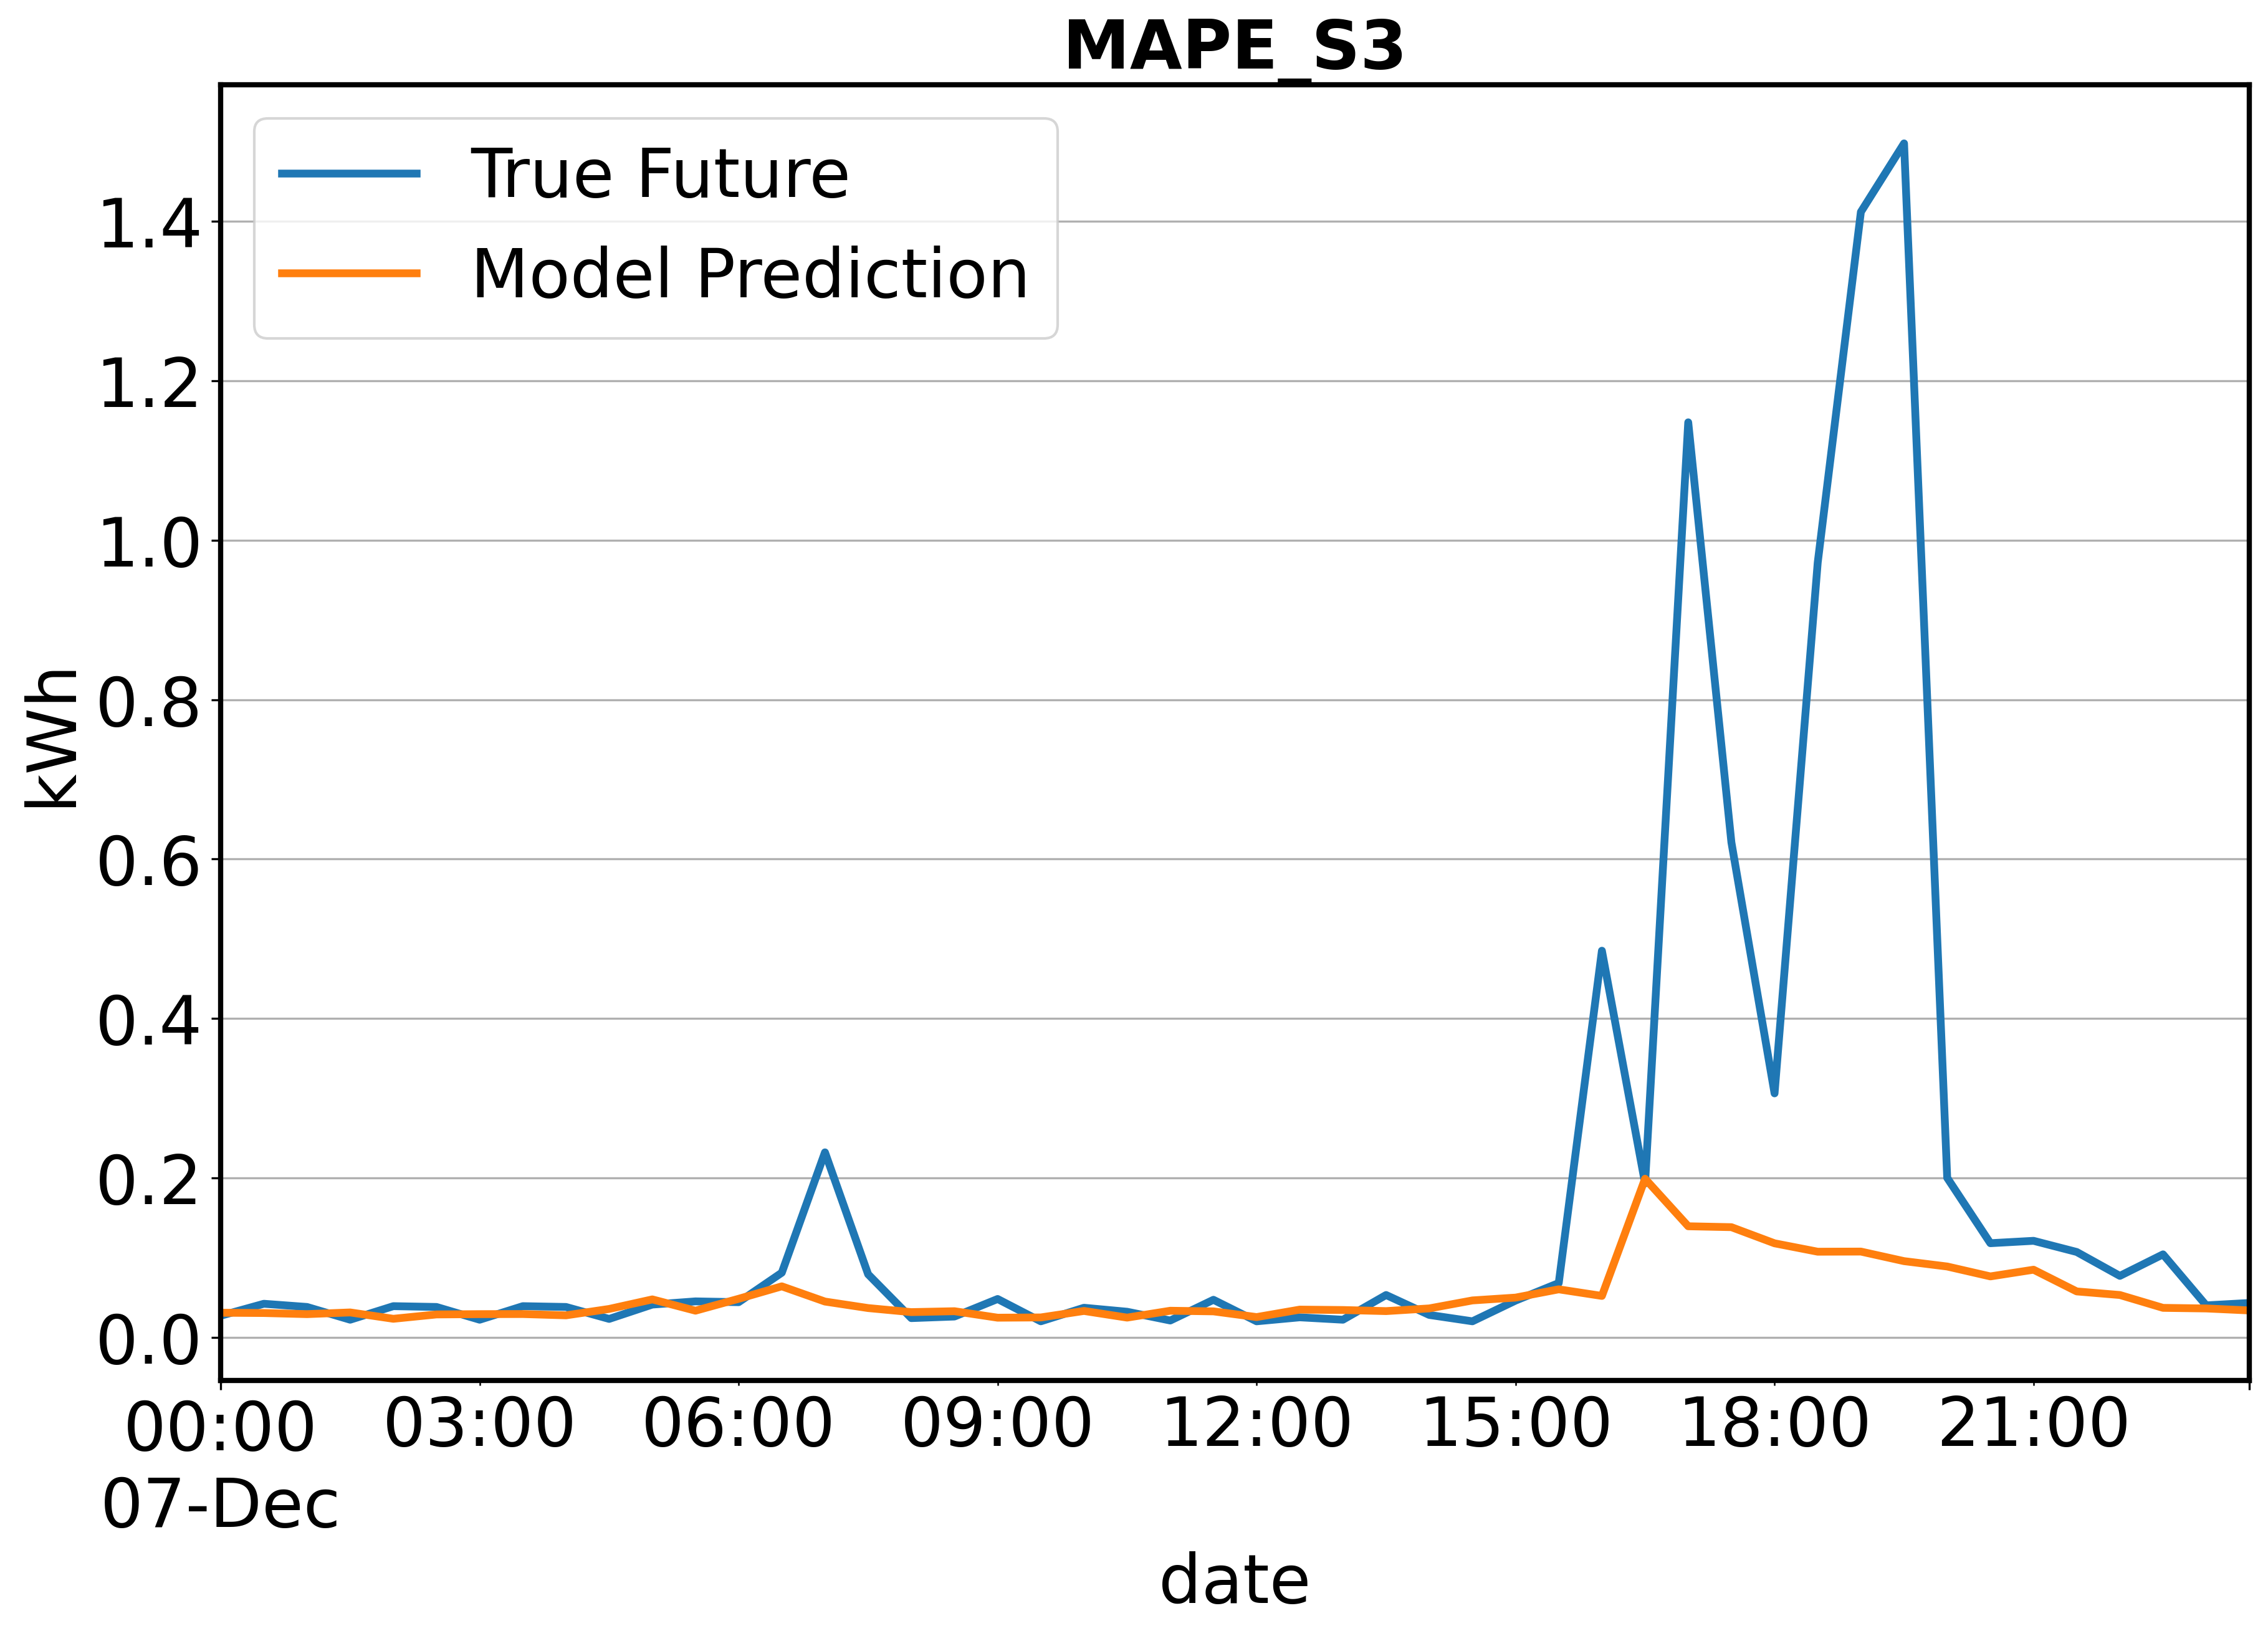
\includegraphics[width=1\linewidth]{IDMAPE_S3_Day341.png}
		\caption{MAPE forecast - Serie $ 3 $}
	\end{subfigure}
 	\caption{The prediction results of the different models on 7th December. (True values: blue/ Prediction: orange)}
 	\label{fig:individual_forecasts}
 \end{figure}


First, it is again stressed that the ``mean squared error'' is chosen as metric during training of the LSTM models. Because of this, the LSTM models are more pushed towards learning the peaks of the reference signal due to the squared error. It can be seen that on the $ 7^{th} $ of December, the peaks of Serie 1 and Serie 3 are present in the predicted signal. It was found that especially for Serie 1, the LSTM models are predicting a higher consumption than the reference signal. The shape of the reference and prediction signals are similar, but there is an offset between the two signals. A reason for the shift could be that the LSTM models are trained using the MSE metric. It is found in literature that when a least square fitting is performed on data points the curve that is fitted can be much disturbed by the presence of outliers. The disturbance resulted also in a shift of the fitted curve. Because during training the MSE is used, the peaks during the day also act as outliers that could be responsible for the model shift. A solution to solve this is to get rid of the squared error and punish more proportional by using the MAE metric instead. On the other hand it can be argued that it is better to predict a higher consumption that one that is too low, because it is better to anticipate to a worse scenario then expected.\\

The reader is reminded that there is no regulation added for Model 1: Serie 1 and Model 3: Serie 1 and 3. When regularization is added this is clearly visible in Figure \ref{fig:individual_forecasts} because without regulation the predicted signal is much more choppy. A clear example can be seen for Model 2 and 3 in serie 3. These two models both show a small bump in the predicted signal before the larger peak. Model 2 where a form of regularization is added shows a very smooth bump while in Model 3 without regularization, the bump is much more choppy. \\

It can be seen that the ``mean forecast'' also is able to identify the two peaks in Serie 1 and the large peak in Serie 3, but as is expected from a mean, this peak is smaller due to averaging. The ``mean forecast'' method however suffers less from the offset than the LSTM models in Serie 1.\\

As expected the ``MAPE forecast'' will focus on correctly predicting the low values in the reference signal because these will get in the denominator of the MAPE metric according to Eq. \ref{eq:MAPE}. It can be seen that the peaks will be ignored when this method is applied. 

\section{Conclusion}
In this chapter the performance of the developed models is assessed. Firstly, the model selection was discussed and it was explained that the models obtained after the parameter search are ran ten times with different initialized weight matrices. The one that performed best on the validation was selected. The number of epochs that the models trained was low, except for model 2 and 3 on Serie 2.\\

 Secondly, the performance on the test set is discussed for the LSTM models and two baseline models using bar plots that displayed the MAE on the test set for each serie. It was concluded that there is a reduction for all the three LSTM models in comparison to both the baseline models for Serie 2 and 3. Also, Model 2 always performed worse based on MAE then the other LSTM models and it can be concluded that the flattening layer didn't have much effect.\\ 
 $ 7 $ December is chosen for which all the predicted signals are grouped for the different models. From this figure is was clear that the LSTM models are able to identify peaks of the reference signal and they have the same overall shape. Predicting the peaks correctly is an important, practical feature e.g. to anticipate electrical peak consumption demands. It was also noticed that the predictions are often an overestimation of the reference signal. Especially for Serie 1, the shape of the reference and prediction signals are similar, but there is an offset between the two signals. The offset could possibly be reduced with another choice of error metric during training. However, it can be a serie dependent effect due to the fact that only for Serie 1 there is a large offset at the start. It can be argued that in practice it is better to overestimate, than underestimate. Because of the overestimation on small values, it was found that the MAPE of the three LSTM neural networks was worse than the baseline models. Also, the influence of adding regularization could be seen which leads to more smooth signals.\\
 
The ``mean forecast'' baseline model was not able to predict the peaks in the reference signal as good as the LSTM models, but it has a lower offset error in Serie 1. The ``MAPE forecast'' is focussed on predicting all the small values correct to minimize the MAPE, but ignores all the peaks of the reference signal.
 


%%% Local Variables: 
%%% mode: latex
%%% TeX-master: "thesis"
%%% End: 
